\documentclass[output=paper]{langsci/langscibook}
\title{Negative existentials in Indo-European: a typological and diachronic overview}
\shorttitlerunninghead{Negative existentials in Indo-European}
\author{Annemarie Verkerk\affiliation{Max Planck Institute for the Science
of Human History\\ Universität des Saarlandes}\lastand
Shahar Shirtz\affiliation{University of Oregon}%
}
% \chapterdoi{}

\abstract{The investigation of the Negative Existential Cycle
\citep{Croft1991} has focused thus far on individual languages and small
language (sub)families. The current paper serves as a starting point to
analyze change in negative existentials and to establish the stability of
the various attested construction types in a larger language family,
Indo-European. Our ultimate objective is to conduct a quantitative
phylogenetic study and this is only possible by consulting a large sample
of related languages. Our first step is to present a typological and
diachronic overview of negative existentials in 42 languages including
Romance, Celtic, Germanic, Baltic, and the Indo-Iranian languages as well
as Albanian, Modern Armenian and Greek. We find that the Romance languages
in our sample are consistently Type A, while the Germanic languages are
consistently Type A{\textasciitilde}B. Indo-Iranian is far more varied and
the most promising branch of Indo-European in terms of providing evidence
for relevant diachronic pathways. We speculate on the reasons for the
stability of Romance's Type A and Germanic's Type A{\textasciitilde}B and
conclude that further phylogenetic analysis of additional languages is
needed from these branches as well as from Indo-Iranian. We present
evidence for the coexistence of two distinct negative existential
constructions in several Indo-Iranian languages and discuss how the
interaction of two or more constructions may contribute to further change
within the Negative Existential Cycle.

\textbf{Keywords:} Negative Existential Cycle, Indo-European, typological
change, Iranian, Indo-Aryan, Germanic, Romance, Celtic}
%
\maketitle
\begin{document}

\section{Introduction}\label{sec:ieur-1}

This paper is an examination of the Negative Existential Cycle (NEC,
\citealt{Croft1991}) in a broad sample of 42
Indo-European\il{Indo-European|(} languages. The
NEC is a typological hypothesis on how special existential negators may
arise and ultimately be used as standard verbal negators. Recent studies by
\textcites{Veselinova2013}{Veselinova2014}{Veselinova2015}{Veselinova2016} who has studied both a large sample of
languages from around the world as well as a wide range of language
(sub)families, show that when considering the actual processes through
which the negators evolve, the NEC often does not take the form of a cycle.
The six stages of the NEC are not necessarily consecutive, as languages can
be split (that is, have different constructions for (existential) negation
belonging to different types), and there is considerable variation in the
stability of these stages. The NEC also interacts with other cycles and
pathways through which negators arise, including Jespersen's Cycle
\parencite[see][]{Gelderen2019}. Existentials are closely related to
locatives \parencites{Clark1978}{Creissels2013ieur}, both conceptually and
concerning the constructions used to encode them (see the introduction to
this volume). 

Cross-linguistic work on the NEC has been mostly limited to
\citegen{Croft1991} original study, to the articles by
\textcites{Veselinova2013}{Veselinova2014}{Veselinova2015}{Veselinova2016}
    and to more general work on negation 
\parencites{KahrelBerg1994}{CyfferEbermann2009}{Budd2010}{WillisLucas2013-ieur}.
The current volume addresses this gap by gathering information on the NEC
in a wealth of different languages and
families. Our contribution focuses on the Indo-European language family,
with the aim to first provide an overview of the constructions that are
used for negative existentials in the various sub-branches of the family,
and second, to analyze the stability of some of these construction types.
We hope that this article contributes to a comparative phylogenetic
analysis in which we can more explicitly test the stability and direction
of change. 

\sectref{sec:ieur-2} of this paper begins with a brief introduction to the
NEC itself, using Indo-European illustrations from the current language
sample, especially from languages that have not been considered in the
literature thus far. In \sectref{sec:ieur-3}, we present and specify the
motivation for the different methods that we used to collect our data as
well as the definitions used in our operationalization of negative
existential clauses. The fourth section is a detailed report on the
different construction types that express a negative existential function
across different branches of Indo-European. This is followed in
\sectref{sec:ieur-5} by some of the diachronic and theoretical
considerations that the data analyzed here raises, and there we argue for
also using evidence from phylogenies when testing pathways of
morphosyntactic change. Finally, we present our conclusions and suggest
several possible directions for future studies.

\section{The Negative Existential Cycle in Indo-European}\label{sec:ieur-2}

The Negative Existential Cycle \citep{Croft1991} is a hypothesis on how
special existential negators may arise and may subsequently evolve into
standard verbal negators. This cycle has six stages \citep{Veselinova2014}
or language types \citep{Croft1991},%
%
    \footnote{We adopt the term ``stage'' when
    discussing the diachronic interpretation of the NEC, and ``type'' when
    referring to the synchronic characterization of a language.}
%
each with a
different relationship between the expression of verbal negation and the
expression of negative existentials:
%
\begin{itemize}
\item Type A: The negative existential construction is the affirmative existential predicate accompanied by the ordinary verbal negator.
\item Type A{\textasciitilde}B: As Type A, but additionally one finds a special negative existential form, often a fusion of the regularly negated existential construction.
\item Type B: Only a special negative existential form exists.
\item Type B{\textasciitilde}C: The special negative existential form begins to be used for ordinary verbal negation.
\item Type C: The negative existential form is the same as the ordinary verbal negator
\item Type C{\textasciitilde}A: The negative existential form + verbal negator begins to be reanalyzed as only a negator, and is used as such in combination with an affirmative existential verb to form a negative existential
\end{itemize}
%
After the negative existential form + verbal negator in Type C{\textasciitilde}A is analyzed as a negator, Type A is reached again and the cycle is complete. The cycle, then, is attempts to make the typology of negative existential constructions more dynamic, providing a diachronic context for each construction type.

We now illustrate each of these types, beginning with Type A, where standard negation is used for both verbal and existential predicates. We illustrate this stage by citing data from Catalan (cat, Romance). Sentential negation in Catalan is expressed by \textit{no} in the preverbal position: 
%
\begin{exe}\ex\label{ex:ieur-catalan-Barcelona}
\langinfo{Catalan}{}{\citealt[154]{Hualde1992}}\\
    \gll en    Joan   no     viu          a   Barcelona \\
\textsc{art}  John    \textsc{neg}   live.\textsc{3sg}   in Barcelona \\
    \glt `John does not live in Barcelona.' %\citep[154]{Hualde1992}
    \end{exe}
%
Existential clauses in Catalan are expressed by a special construction that uses \textit{haver-hi} `there is', literally `there has,' where \textit{hi} is a locative adverbial clitic. This construction is similar to other clauses in Catalan and is negated by a preverbal \textit{no}: 
%
\begin{exe}\ex\label{ex:ieur-catalan-possibilities}
\langinfo{Catalan}{}{\citealt[460]{WheelerYates1999}}\\
    \gll hi      ha                  tres   possibilitats.  \\
there have.\textsc{prs}.\textsc{3sg} three possibility.\textsc{pl} \\
    \glt `There are three possibilities.' 
\ex\label{ex:ieur-catalan-copying}
\langinfo{Catalan}{}{\citealt[422]{WheelerYates1999}}\\
    \gll No hi ha cap examen on no enxampin algú copiant.  \\
\textsc{neg}   there have.\textsc{prs.3sg}   any exam 
where \textsc{neg}   catch.\textsc{sbj.3pl}   somebody  copy.\textsc{ger}\\
    \glt `There is no exam where they don't catch somebody copying.' 
    \end{exe}
%
In the second stage (Type A{\textasciitilde}B), a special negator is used
for existential sentences that only occur in specific contexts (see the
discussion below on details regarding the variation allowed in the usage of
the special negator). An example of this type is Sivandi (siy, Central
Iranian). The Sivandi standard negation marker is a \textit{na}(\textit{y})- or
\textit{ne}(\textit{y})- prefix \citep[69]{Lecoq1979}. Sivandi negative existentials
can be formed by \textit{dār-} `be located, be at, have' or the past tense
copula \textit{bi} as illustrated in \REF{ex:ieur-sivandi-woman}. The existential
markers can be negated by the standard preverbal negator \textit{na}-,
\textit{ne}-, \textit{ney}- as in \REF{ex:ieur-sivandi-electricity}:
%
\begin{exe}\ex\label{ex:ieur-sivandi-woman}
\langinfo{Sivandi}{}{\citealt[85]{Lecoq1979}}\\
    \gll ye    pīrežen=i                 bi \\
one old.woman=\textsc{indef}   be.\textsc{pst.3sg} \\
    \glt `There was an old woman.'
\ex\label{ex:ieur-sivandi-electricity}
\langinfo{Sivandi}{}{\citealt[89]{Lecoq1979}}\\
    \gll albatta   barqa=m      na=bi \\
evidently   electricity=\textsc{top}   \textsc{neg}=be.\textsc{pst.3sg} \\
    \glt `(Someone lit a candle), evidently there was no electricity.'
    \end{exe}
%
Sivandi also has a special negative copula form, \textit{nūnd}, which is historically composed of the negation marker \textit{ne-} added to another element, the exact identity of which is still unclear. This is a negative copula form that is used as the negative counterpart of the Present tense copula:
%
\begin{exe}\ex\label{ex:ieur-sivandi-hand}
\langinfo{Sivandi}{}{\citealt[150]{Lecoq1979}}\\
    \gll vāllāh, me    či     tū das=em      nūnd \\
by.god  \textsc{1sg}  what in hand=\textsc{1sg}   \textsc{neg.cop} \\
    \glt `By God, there's nothing in my hand'
    \end{exe}
%
The existential predicates in the next construction type, Type B, are not
negated by the standard negator, but only through a special strategy. One
example of a Type B language is Kurmanji\il{Kurmanji} Kurdish [kmr]. In Kurmanji, a
preverbal marker \textit{na-}, \textit{ne-}, considered to be either a
prefix or clitic, is used for standard negation:
%
\begin{exe}\ex
\langinfo{Kurmanji}{}{\citealt[35--36]{Thackston2006}}\\  
    \gll ez      na=tʃ-im             doctor \\
\textsc{1sg}   \textsc{neg}=go.\textsc{prs}-\textsc{1sg}    doctor \\
    \glt `I am not going to the doctor.'
    \end{exe}
%
The affirmative existential construction consists of a single-figure constituent followed by the regular copula:
%
\begin{exe}\ex\label{ex:ieur-kurmanji-ancestors}
\langinfo{Kurmanji}{}{\citealt[31]{Thackston2006}}\\
    \gll Got-in-eke pêşiy-ên      me   heye.  \\
say-\textsc{nmz}-cnst.\textsc{indef} ancestor-\textsc{pl} \textsc{1pl.obl}   be.\textsc{prs.3sg} \\
    \glt `There is a saying of our ancestors.' 
    \end{exe}
%
The negative existential does not take the form of a negated affirmative existential construction, but is formed by using the special verb \textit{tun-}:
%
\begin{exe}\ex\label{ex:ieur-kurmanji-authority}
\langinfo{Kurmanji}{}{\citealt[32]{Thackston2006}}\\
    \gll Di vî warî    da otorîtey-eke resmî   tune.  \\
in  \textsc{dem}    regard in  authority-cnst.\textsc{indef}  official \textsc{cop.neg.prs.3sg} \\
    \glt `In this regard, there is no official authority.' 
    \end{exe}
%
For Type B{\textasciitilde}C, the special existential negator is also used
under certain conditions to negate some verbal predicates. In the current
sample, Type B{\textasciitilde}C is attested in Oriya (ory, Eastern
Indo-Aryan), but its description is slightly complicated. We will discuss
this further in \sectref{sec:ieur-4.1}. \citet{Veselinova2014} has
described two other Type B{\textasciitilde}C Indo-European languages,
Bulgarian\il{Bulgarian} [bul] and Macedonian\il{Macedonian} [mkd]. \citet[1332--1333]{Veselinova2014}
offers the following examples and analysis for Bulgarian. The standard
negator generally found in Slavic and specifically in Bulgarian is the
pre-verbal particle \textit{ne} (ex.
\ref{ex:ieur-bulgarian-negators}a--b). The existential negator,
however, is \textit{njama}, which is a reduction of the third person
singular of the verb \textit{imam} `to have' (ex.
\ref{ex:ieur-bulgarian-negators}c--d). The form
\textit{njama} is used in the future tense as a standard negator (ex.
\ref{ex:ieur-bulgarian-negators}e--f), that is, only under specific conditions. That is, \textit{njama} is
not restricted to negative existentials.
%
\begin{exe}\ex\label{ex:ieur-bulgarian-negators}
\langinfo{Bulgarian}{}{\citealt[1332--1333]{Veselinova2014}}
\begin{xlist}
\ex
    \gll Maria pee \\
Maria sing.\textsc{3sg}.\textsc{prs} \\
    \glt `Maria sings.'
\ex
\gll Maria ne pee \\
Maria \textsc{neg} sing.\textsc{3sg}.\textsc{prs} \\
\glt `Maria does not sing.'
\ex\gll Ima div-i kotk-i \\ 
   have.\textsc{3sg}.\textsc{prs} wild-\textsc{pl} cat-\textsc{pl} \\
\glt `There are wild cats.'
\ex\gll Njama div-i kotk-i \\
not.have.\textsc{3sg}.\textsc{prs} wild-\textsc{pl} cat-\textsc{pl} \\
\glt `There aren't any wild cats.'
\ex\gll Dovečera shte xodja na kino \\
tonight     \textsc{fut} go.\textsc{1sg}.\textsc{prs}  to cinema \\
\glt `I will go to the movies tonight.'
\ex\gll Dovečera njama                  da   xodja          na  kino\\
tonight not.have.\textsc{3sg}.\textsc{prs} sub go.\textsc{1sg.prs} to
cinema \\
\glt `I will not go to the movies tonight.'
    \end{xlist}\end{exe}
%
In the following stage, Type C, the special existential negator is commonly
used for negative verbal predicates but replaces the affirmative
existential marker rather than combining with it. There are several Type C
negative existential constructions in Indo-European languages, particularly
in Indo-Iranian languages, and this is illustrated more thoroughly in
\sectref{sec:ieur-4.1}. Here, we demonstrate this pattern by citing
examples from Kupia\il{Kupia} (key, Eastern Indo-Aryan), spoken in Northern Andhra
Pradesh. In \REF{ex:ieur-kupia-tiger} \textit{nay} is used as the verbal
negation marker. In \REF{ex:ieur-kupia-market} \textit{nay} is used as the negative existential copula:
%
\begin{exe}\ex\begin{xlist}
\ex\label{ex:ieur-kupia-tiger}
\langinfo{Kupia}{}{\citealt[38]{Christmas1973b}}\\
    \gll anne nig-e          nay \\
            and   run-\textsc{3sg}      \textsc{neg} \\
    \glt `(The tiger stood up) and didn't run.'
\ex\label{ex:ieur-kupia-market}
\langinfo{Kupia}{}{\citealt[23]{Christmas1973b}}\\
\gll iːndʒa santa-yi ne dorku ja-t-i wastuwu nay\\
    \textsc{dem}     market-\textsc{loc} \textsc{neg} available
    become-\textsc{prs-f}
goods      \textsc{neg}\\
\glt `There are no goods that aren't available at the market.'
\end{xlist}\end{exe}
%
The final stage, Type C{\textasciitilde}A, represents a further step in
that the special existential negator combines with the affirmative
existential construction to form the negative existential construction,
however the result is emphatically or pragmatically marked.
\citegen{Croft1991} example of a Type C{\textasciitilde}A language is an
Indo-Aryan language, Marathi\il{Marathi} [mar], where the negative existential form
\textit{nāhi} can function as the negative existential, but it also can
combine with the positive existential \textit{āhe}:
%
\begin{exe}\ex\label{ex:ieur-marathi-anyone}
\langinfo{Marathi}{}{\citealt[12, p.c. Madhav Deshpande,
Croft's glosses]{Croft1991}}
\begin{xlist}
\ex
    \gll tithǝ  koṇi      āhe \\
there anyone \textsc{ex} \\
    \glt `Is anyone there?'
\ex
\gll koṇi      tithǝ  dzāt {\ob}ǝts{\cb}     nāhi\\
anyone there goes [\textsc{emph}] \textsc{neg}\\
\glt `Nobody goes there.'
\ex
\gll tithǝ  koṇi      nāhi {\ob}āhe{\cb}\\
there anyone \textsc{neg}  [\textsc{ex}]\\
\glt `There isn't anyone there.'
\end{xlist}\end{exe}
%
\citet[12]{Croft1991} states that the negative existential construction
that contains both \textit{nāhi} and \textit{āhe} is more emphatic than the
construction with only \textit{nāhi}, suggesting that the construction that
combines the two is more recent. The Negative Existential Cycle is complete
once the emphatic or pragmatic markedness of the combination of the former
special existential negator and the affirmative existential wears off. We
then return to Type A, where a standard negator is used for both verbal and
existential predicates. 

\citet{Croft1991} analyzed a sample of 23 unrelated languages and drew on
general diachronic processes to infer the directionality of change and to
propose the Negative Existential Cycle \parencite[3--4, 13ff]{Croft1991}.
This has since been investigated more directly by
\textcites{Veselinova2013}{Veselinova2014}{Veselinova2015}{Veselinova2016},
who has analyzed a large sample of languages throughout the world as well
as a large range of language (sub)families to determine the
historical processes therein. The analyses by Croft and Veselinova of some
negative existential construction types differ. For example, to describe
stage A{\textasciitilde}B, \citet[6--12]{Croft1991} emphasizes the existence
of a construction with a special negative existential form in addition to a
construction with the standard verbal negative marker. In contrast,
\citet[1328]{Veselinova2014} emphasizes that the special form is limited to
specific contexts, depending on factors such as tense or aspect.
Furthermore, \citet[136--138]{Veselinova2013} argues that special negative
existential markers (that is, those implicated in Type B constructions),
can arise through multiple processes and only some of them are directly
connected to Croft's cycle. These points highlight the differences between
the three transitional construction types. While Type A{\textasciitilde}B
requires the co-existence of two constructions, one of Type A and one of
Type B, Types B{\textasciitilde}C and C{\textasciitilde}A are defined by
the distinct uses of the negative existential marker, and therefore do not
require the existence of two negative existential constructions.

The most important conclusions of Veselinova's investigations are
summarized in \citet[170ff]{Veselinova2016}. First, the types identified in
the Negative Existential Cycle are construction types rather than language
types because we find that these types co-occur within the same language.
\citet[1372--1373, 1343ff]{Veselinova2014} first identifies these split
languages in the Polynesian subfamily, and later notes that the most common
split type is A{\textasciitilde}B\slash B{\textasciitilde}C \citep[154]{Veselinova2016}. Below, we further identify such co-occurrences in Indo-European, offering additional support for Veselinova's findings.

Second, the six types of the Negative Existential Cycle do not necessarily
present a diachronic sequence. Veselinova
(\cite*[1336--1337]{Veselinova2014}; see also
\citealt[22]{Croft1991}) demonstrates that while Bulgarian (see ex.
\ref{ex:ieur-bulgarian-negators}
above) and Macedonian are excellent examples of the transitional Type
B{\textasciitilde}C, whereas all other Slavic languages are either Type A
or Type A{\textasciitilde}B, Bulgarian and Macedonian are not examples of
the Negative
Existential Cycle at work, as they have not gone through stage B. A similar
story can explain changes in the distribution of the Russian special
negator \textit{net} \parencite[1335, 1337--1338]{Veselinova2014}. Aside
from these ``gaps'' in the Cycle, \citet[127]{Veselinova2013} first observes
that as an alternative route to the Negative Existential Cycle, special
negative existential forms can change into standard negation markers when
they are used as pro-sentences (`Are you at home?' `No [, I am not at
home]') and later on as general words for `no' \citealt[see
also][1339]{Veselinova2014}. Subsequent analysis in
\citet[155ff]{Veselinova2016}
 reveals at least three other attested diachronic processes. This
means that the Negative Existential Cycle is not the only diachronic
process through which special negative existential forms can enter the
domain of standard negation.  

The third and last point is that an analysis of the Negative Existential
Cycle that is based on a language family from a historical-comparative
perspective has consequences for our understanding of the stability of the
various construction types and the rate of change between them
\parencites[577]{Veselinova2015}[170]{Veselinova2016}. Through the course
of her investigation, \citet[150]{Veselinova2016} finds that the
``transitional'' stages A{\textasciitilde}B and B{\textasciitilde}C are
cross-linguistically more common than the ``non-transitional'' stages of C
and A. These ``transitional'' stages can be maintained for extended periods
of time, which
also accounts for their synchronic dominance. \citet{Veselinova2016}
reports on an accumulation of findings on the Negative Existential Cycle in
six language (sub)families, but only one of these (Polynesian) features all
six types. The Polynesian subfamily has diverged only relatively recently
(approximately 2,000 years ago). \citet[155]{Veselinova2016} suggests that
the type of subordination construction that several Polynesian languages
used for negation has been conducive to frequent renewal and rapid change
in this family. This stands in contrast to several other, older families --
Berber, Dravidian, Uralic -- where only a few types of the Negative
Existential Cycle are attested \parencite[see][147--149]{Veselinova2016}.
Hence, changes that occur within the Negative Existential Cycle as well as
through other processes that result in special negative existential forms
expressing standard verbal negation, depend on the language or language
family-specific characteristics
\parencites[154]{Veselinova2016}[1373]{Veselinova2014}. This position is in
line with current research in typology that demonstrates that language
families have their own lineage-specific trends,
both regarding features that tend to be stable and correlated with each
other \parencites{DunnGreenhill2011}{DediuLevinson2012}{Bickel2013}. 

The aim of the current paper is to present a first preliminary overview of
the constructions that are used for negative existentials in the various
sub-branches of the Indo-European language family. In the future, we intend
to expand the dataset to conduct an analysis using phylogenetic comparative
methods. As \citet{Veselinova2013} has demonstrated in a worldwide sample
of 95 languages, Western Europe is not a particularly exciting place to
investigate negative existential constructions, as the Western-European
branches of Indo-European are relatively uniform in terms of the
construction types that express the negative existential
domain.%
%
\footnote{This is not an exceptional pattern, considering for instance
clause alignment patterns, where Western European languages are uniformly
accusative \citep{Siewierska2013}, while the Indo-Iranian languages display
considerable variation \parencites{Haig2008}{Verbeke2013}.} 
%
Nevertheless, our objective is to contribute to
the current set of family-based historical-comparative studies. We decided
to investigate Indo-European languages despite the limited variation in
Western Europe for three, specific reasons. First, this is a large family
that has been widely and extensively documented, which unlocks the
potential to discover the entire cycle. Additionally, while the
Indo-European languages of Western Europe are not especially varied, the
Indo-Iranian languages do display interesting variation. Finally, there is
also potential for an analysis of the interactions between some
Indo-European branches and Uralic and Dravidian language families, which
have already been studied by Veselinova (2015, 2016) as well as the Semitic
and Tibeto-Burman families. 

\section{Methodology}\label{sec:ieur-3}

The negative existential, like other domains of nominal predication, tends
to be under-reported in published grammatical descriptions, either in the
form of full reference grammars or grammar sketches. To overcome this, this
study uses a combination of data sources to increase the coverage in terms
of languages and branches. We included languages from each major branch of
Indo-European, based on the likelihood of materials and experts being
available in an attempt to establish a wide genealogical and geographical
coverage. For example, we include Indo-Aryan languages from the Eastern,
Northern, and Southern Zones, as well as Central and Western Iranian
languages. To obtain the broadest language sample possible at this time,
our sources include reference and sketch grammars as well as data from an
analysis of published textual material and data from a translation
questionnaire.

The translation questionnaire was slightly adjusted from
\citet{Veselinova2014} (\citealt{Veselinova2014}, Appendix C) and is
included in Appendix A. Those experts and colleagues who have completed the
translation questionnaire for their native language or their language of
expertise are mentioned by name unless they preferred to remain anonymous.
The questionnaire elicits translations of many different types of clauses,
both affirmative and negative. Besides existential clauses, the
questionnaire includes clauses that are expected to be completely verbal,
such as ``Marie sang.'' or ``Marie didn’t sing.'' and clauses which belong
in the domain of nominal predication (as defined, for example, in
\citealt[111--127]{Payne1997}) such as “Tom is tall.” or “Tom isn’t tall.”.
This allowed us to evaluate the similarities in the expression of negation
across different functional and grammatical domains. We then typically
asked follow-up questions and elicited further grammatical patterns that
express negative existence. For example, having identified a specific
pattern in the expression of negative existential in one language (such as
an A{\textasciitilde}B split that is based on tense), we can probe whether
similar patterns exist in other closely related languages. 

The third data source we consulted consists of published naturalistic
texts. We find that the direct use of texts aids us in analyzing many
similarly ``minor'' functions (such as other specific subdomains of nominal
predication) or even ``major'' functions such as discourse functions, which
tend to not make their way to reference grammars. This is not a critique of
grammar writing practices -- good grammars are often long and sufficiently
detailed. They cannot and should not be expected to cover all functional
domains that future linguists may potentially inquire about. The fact that
many reference grammars are sufficiently detailed to enable linguists to
directly consult primary texts testifies to the superb quality of these
grammatical descriptions.

The analysis of primary textual data from a variety of languages is rather
the reality of researching constructions or functions that have not been
thoroughly analyzed either in a typological or a descriptive sense. This is
a labor-intensive task, but it is aided here by the fact that negative
existence is often expressed by similar, even cognate, grammatical means,
and that the grammatical patterns are similar to a large degree. The
textual analysis also allows us to discern the common discourse situations
that the negative existential constructions occur in, which often involve a
change of location or a shift in the deictic center.

We do not see an apriori advantage to any of the three types of data
sources used here. Yet the reality is that grammatical descriptions tend to
not mention grammatical patterns that express the negative existential
domain and negative existential clauses have a very low frequency in
naturalistic texts. Thus, even when information from different sources was
(at least potentially) available, we gave precedence to information from
native speakers or language experts.  

As demonstrated by \citet[112ff]{Veselinova2013} and by her subsequent
work, the type of negative existential construction is identified by
comparing the
negation strategies of existential constructions to that of standard verbal
predicates. Of special importance here are locative sentences which are
often encoded by very similar constructions but must be conceptually
distinguished. This difference is found in the information status of the
subject and the perspective on the figure-ground relationship between
figure and the ground (p.c. Ljuba Veselinova, \citealt{Creissels2013ieur}):
%
\begin{exe}\ex\label{ex:ieur-book-on-the-table}
predicate location: The book is on the table.\\
existence: There is a book (on the table).
    \end{exe}
%
The figure entity of a locative predicate tends to be given information or
be identifiable in context, while the comparable entity of an existential
predicate is indefinite, potentially indicating new information that is not
usually mentioned or referred to in the text immediately preceding the
clause. The locative predicate establishes the location of an entity while
the existential predicate is used to predicate the existence of an entity
relative to a specific, often identifiable, location \citep{Creissels2013ieur}.
Creissels' \citeyearpar{Creissels2013ieur} conceptualization of existentials avoids positing
their semantics, that is, the notion that existential predicates assert or
deny the existence of something, as their main defining property
\parencite[6ff]{Creissels2013ieur}. Nevertheless, in our search for existential
predicates, we attempted to find and elicit as many examples as possible,
both with and without an explicit location present (`on the table'), in an
attempt to ensure that the two are considered separately in our analysis.
When their encoding diverges, we are interested in existentials only and do
not include details on locatives. 

\section{Typological overview}\label{sec:ieur-4}

In this section, we survey negative existentials that occur in the major
Indo-European branches, moving from East to West. We begin with
Indo-Iranian and end with Celtic. This section does not feature all the
languages we collected data on. In Appendix B, we present a full overview
of all 42 languages we investigated and provide examples and source
information in the same order of branches. For ease of presentation, given
the large number of scripts involved, we use transcriptions or
transliterations into the Latin script in all examples. 

\subsection{Indo-Iranian}\label{sec:ieur-4.1}

This section surveys the different negative existential construction types
attested in a sample of Indo-Iranian\il{Indo-Iranian|(} languages. The
survey reveals that across Indo-Iranian, all six types of negative
existential constructions in \citegen{Croft1991} cycle occur and that
different construction types co-exist in some languages: most notably A and
B (essentially instances of Croft's Type A{\textasciitilde}B) or C and A
(essentially instances of Croft's Type C{\textasciitilde}A), but also A \&
B{\textasciitilde}C or B \& C. These results are summarized in
\tabref{tab:ieur-class-Indo-Iranian} below.
Considering the attested combinations of states, together with the
combinations found in Polynesian languages \citep{Veselinova2014}, we argue
in \sectref{sec:ieur-5} below that at least some of the unattested
combinations thus far might be the result of the definitions of the
different construction types. 

\begin{table}\begin{small}
\caption{Overview of classification of Indo-Iranian languages}
\label{tab:ieur-class-Indo-Iranian}
\begin{tabularx}{\textwidth}{@{} l p{23mm} l l l Q @{}}
\lsptoprule
\textbf{Language} & \textbf{Genealogical} & \textbf{Iso-}&
\textbf{Glottolog} & \textbf{Classifi-} & \textbf{Source(s)}\\ 
&\textbf{Affiliation} &\textbf{code} &\textbf{code}&\textbf{cation} \\
\midrule
Old & Old Iranian & peo & oldp1254 & A & Primary texts \\
Persian & & & & &(inscriptions)\\
\midrule
Middle & Western Middle & pal & pahl1241 & A{\textasciitilde}B & Primary texts \\
Persian & Iranian & & & &(Zoroastrian MP)\\
\midrule
Tajik & Western Iranian & tgk & taji1245 & A{\textasciitilde}B & Own data, \citealt{Perry2005}\\
\midrule
New & Western Iranian & pes & west2369 & A{\textasciitilde}B & Own data\\
Persian \\
\midrule
Sivandi & Central Iranian & siy & siva1239 & A{\textasciitilde}B & \citealt{Lecoq1979}\\
\midrule
Gorani & Central Iranian & hac & gora1267 & A{\textasciitilde}B &
\citealt{MahmoudveysiBailey2012}\\
\midrule
Gilaki & Central Iranian & glk & gila1241 & A &
\citealt{RastorguevaKerimova2012} \\
\midrule
Ziyarati & Central Iranian & mzn & maza1291 & A & \citealt{ShokriJahani2013} \\
\midrule
Kurmanji & Central Iranian & kmr & nort2641 & B & \citealt{Thackston2006} \\
\midrule
Taleshi & Central Iranian & tly & taly1247 & C{\textasciitilde}A & \citealt{Paul2011}\\
\midrule
Koroshi & Central Iranian & ktl & koro1296 & A{\textasciitilde}B &
\citealt{NourzaeiJahani2015} \\
\midrule
Hindi & Central Zone\newline Indo-Aryan & hin & hind1269 & C{\textasciitilde}A & \citealt{Bashir2006}, \textit{godaan} by Munshi Premchand\\
\midrule
Odia & Eastern Zone\newline Indo-Aryan & ory & oriy1255 & A \& B{\textasciitilde}C & \citealt{NeukomPatnaik2003} \\
\midrule
Assamese & Eastern Zone\newline Indo-Aryan & asm & assa1263 & A{\textasciitilde}B & p.c Nihankara Dutta, Krishna Boro\\
\midrule
Kupia & Eastern Zone\newline Indo-Aryan & key & kupi1238 & B \& C & \citealt{Christmas1973a}, b \\
\midrule
Marathi & Southern Zone\newline Indo Aryan & mar & mara1378 & C{\textasciitilde}A & \citealt{Croft1991}\\
\midrule
Nepali & Northern Zone\newline Indo-Aryan & npi & nepa1254 & A & p.c Sugam Singh\\
\lspbottomrule
\end{tabularx}
\end{small}\end{table}
%
Many Indo-Iranian languages express the affirmative existential domain by a
combination of a copular verb and a NP expressing the existing entity. This
is illustrated by the clauses in examples \REF{ex:ieur-persian-people} and
\REF{ex:ieur-assamese-wildcats}, which are from Middle Persian\il{Middle Persian} (pal,
Western Iranian, circa 3rd century CE -- 9th century) and
Assamese\il{Assamese} (asm,
Eastern Indo-Aryan).
The functional range of the copular verbs in these two clauses is not
limited to clauses that express the existential domain but also includes
other nominal predication domains.
%
\begin{exe}\ex\label{ex:ieur-persian-people}
Middle Persian\il{Middle Persian} (AWN 9.2)\\
    \gll ud  mardōm bud     hēnd \\
and people   be.\textsc{pst} be.\textsc{prs}.\textsc{3pl} \\
    \glt `And there were people (who were as bright as the sun).'
\ex\label{ex:ieur-assamese-wildcats}
\langinfo{Assamese}{}{p.c. Nihankara Dutta, Krishna Boro}\\
    \gll bonoria mekuri as-e \\
wild       cat       \textsc{cop}-\textsc{3sg}.\textsc{prs} \\
    \glt `There are wild cats (in the world).'
    \end{exe}
%
Much of the variation in the expression of the negative existential in
Indo-Iranian is the result of different types of interaction between some
form of the verbal copula and a standard verbal negation marker. In many
constructions across the Indo-Iranian languages, the standard verbal
negation marker simply accompanies the copular verb. In other
constructions, morphological reduction of the two leads to univerbation and
to the emergence of innovative negative copulas or innovative verbal
negation markers. Other factors that increase the crosslinguistic variation
in this domain are the rise of innovative locative copulas, usually labeled
as `stay,' `exist (in)' or `be at,', and innovative negation markers.
Rather than describing the different construction types attested in each
language, the focus of this section is on examples that illustrate
instances of each different construction type across the family.

In Old Persian\il{Old Persian} [peo], the standard negation marker \textit{naiy} is
deployed in a preverbal position. The Old Persian affirmative existential
is expressed by a copula accompanied by a NP expressing the existing
entity, similar to the two clauses in examples \REF{ex:ieur-persian-people}
and \REF{ex:ieur-assamese-wildcats} above. Clauses that express the
negative existential in
Old Persian, while apparently rare, are composed of a combination of the
standard verbal negation marker \textit{naiy} followed by the verbal
copula. These two are accompanied by a NP that conveys the existing entity,
as illustrated by example \REF{ex:ieur-persian-no-man}. Negative
existential clauses in Old Persian are therefore an instance of Croft's
Type A construction.
%
\begin{exe}\protectedex{\ex\label{ex:ieur-persian-no-man}
Old Persian\il{Old Persian} (DB1:48--49)\\
    \gll naiy  āha martiya    naiy  pārsa   naiy māda … \\ 
\textsc{neg} \textsc{cop}.\textsc{pst}.\textsc{3sg} man     \textsc{neg}
persian \textsc{neg} median \\
    \glt `there was no man, not Persian, not Median, (… who dared to speak
up)'}
\end{exe}

This situation is common across the Indo-Iranian languages, and it is
responsible for many occurrences of Type A constructions. In the (a--b)
pairs in examples
(\ref{ex:ieur-persian-sin-fire}--\ref{ex:ieur-ziyarat-understand-watchmen})
below, the clauses in (a) illustrate the standard verbal negation marker as
it occurs in Middle Persian\il{Middle Persian} [peo], Sivandi\il{Sivandi} [siv],
and Ziyarati\il{Ziyarati} [maz]
(Sivandi was also discussed in \sectref{sec:ieur-2}). The clauses in (b)
illustrate a negative existential construction in each language. Across
these pairs, the verbal negation marker in (a) is the same negation marker
deployed in (b). The straightforward difference between the Middle
Persian\il{Middle Persian}
affirmative existential in example \REF{ex:ieur-persian-people} above, and
the negative existential in example \REF{ex:ieur-persian-fire} below, is
the presence of the standard negation marker that occurs in a preverbal
position.
%
\begin{exe}\ex\label{ex:ieur-persian-sin-fire}
\begin{xlist}
\ex
Middle Persian\il{Middle Persian} (DK6:50)\\
    \gll wināh nē    kun-ēd \\
sin \textsc{neg} do.\textsc{prs}-\textsc{3sg} \\
    \glt
`He will not sin.'
\ex\label{ex:ieur-persian-fire}
Middle Persian\il{Middle Persian} (PRDD:18a)\\
\gll agar ātaxš ī        wahrām  nē     būd\\
if fire \textsc{lnk} Wahram \textsc{neg}  be.\textsc{pst}.\textsc{3sg}\\ 
\glt `If the fire of Wahram did not exist. (lit. if there was no fire of Wahram)'
\end{xlist}
\ex\begin{xlist}
\ex\label{ex:ieur-sivandi-gardens}
\langinfo{Sivandi}{}{\citealt[90]{Lecoq1979}}\\
    \gll ū bāγ-gar-i mardem na=šu \\
\textsc{3sg} garden-\textsc{pl}-\textsc{lnk}   people    \textsc{neg}=go.\textsc{pst}.\textsc{3sg} \\
    \glt `He did not go into the gardens of those people.'
\ex
  \langinfo{Sivandi}{}{\citealt[89]{Lecoq1979}}\\
\gll albatta   barqa=m      na=bi\\ 
evidently electricity=\textsc{top}
\textsc{neg}=be.\textsc{pst}.\textsc{3sg}\\
\glt `(someone lit a candle), Evidently there was no electricity.'
\end{xlist}
\protectedex{
\ex\label{ex:ieur-ziyarat-understand-watchmen}\begin{xlist}
    \ex
\ili{Ziyarati} Mazandarani \parencite[26]{ShokriJahani2013}\\ 
    \gll te harf=am na{-it-i} \\
\textsc{2sg} word=\textsc{1sg} \textsc{neg}-get.\textsc{pst}-\textsc{2sg}\\
    \glt `You did not understand my words.'
\ex
\ili{Ziyarati} Mazandarani \parencite[84]{ShokriJahani2013}\\ 
\gll ʃupā da-ni-bu-in …\\
watchman  \textsc{prv}-\textsc{neg}-be.\textsc{pst}-\textsc{3pl}\\
\glt `(if) there are no watchmen'
\end{xlist}}\end{exe}

Locative verbs, often understood to mean something like `stay,' `exist
(in)', or `be at', are usually negated by the standard negation marker. The
(a) clauses in examples \REF{ex:ieur-assamese-sing-nowildcats} and
\REF{ex:ieur-gilaki-make-nocars} illustrate
the standard verbal negation markers that occur in Assamese\il{Assamese}
[asm] and Gilaki\il{Gilaki} [glk], and their (b) counterparts show that
this marker is used to negate locative verbs in the negative existential
pattern. The Sivandi\il{Sivandi}
standard negation marker, a preverbal \textit{na=}, as illustrated by
\REF{ex:ieur-sivandi-gardens} above, also occurs in
\REF{ex:ieur-sivandi-nograin} in a negative
existential clause, with an innovative locative verb.
%
\begin{exe}
    \protectedex{
\ex\label{ex:ieur-assamese-sing-nowildcats}\begin{xlist}
\ex
\langinfo{Assamese}{}{p.c. Nihankara Dutta, Krishna Boro}\\
    \gll mohila-goraki{\op}-e{\cp}   gan   na-ga-j \\
woman-\textsc{clf}-(\textsc{nom}) song  \textsc{neg}-sing-\textsc{3sg}\\
    \glt `The woman didn't sing.'
\ex\label{ex:ieur-assamese-nowildcats}
\langinfo{Assamese}{}{p.c. Nihankara Dutta, Krishna Boro}\\
\gll bonoria mekuri na-tʰak-e\\
wild cat \textsc{neg}-stay-\textsc{3sg}.\textsc{prs}\\
\glt `There are no wild cats.'
\end{xlist}
\ex\label{ex:ieur-gilaki-make-nocars}\begin{xlist}
\ex\label{ex:ieur-gilaki-make}
\langinfo{Gilaki}{}{\citealt[125]{RastorguevaKerimova2012}}\\
    \gll nə-kun-əm \\
\textsc{neg}-do.\textsc{prs}-\textsc{1sg} \\
    \glt `I do not make'
\ex
\langinfo{Gilaki}{}{\citealt[326]{RastorguevaKerimova2012}; their glosses
and parsing}\\
\gll mašin nə-ø-na-ø \\
car \textsc{neg}-\textsc{prf-}exist.\textsc{pst}-\textsc{3sg.pst}\\
\glt `There are no cars.'
\end{xlist}
%\end{exe}\begin{exe}
            \ex\label{ex:ieur-sivandi-nograin}
\langinfo{Sivandi}{}{\citealt[150]{Lecoq1979}}\\
    \gll ke   bār   na=dār-e \\
\textsc{comp}   grain  \textsc{neg}=be.at-\textsc{3sg} \\
    \glt
`(He closed his windmill down) because there was no grain.'
}\end{exe}

So far, the examples for Croft's Type A constructions all involve preverbal
negation markers, which are commonly found across Indo-Iranian languages.
However, many Indo-Aryan languages underwent different historical processes
that resulted in changes in the relative order of the negation marker and
the negated verb. This is illustrated by example \REF{ex:ieur-nepali-window} below
from Nepali\il{Nepali} [npi], where the post-verbal negation marker is essentially
suffixed to the verb.%
%
\footnote{This is a rather simplified picture of
polarity in the Nepali verb, but other negation markers behave similarly
with respect to the variables analyzed here.} 
%
The predicates in the negative existential clauses in examples
(\ref{ex:ieur-nepali-window-nocats}b--c) differ in the type of
copular verbs, but both are negated by the same marker used with finite
verbs, as in example \REF{ex:ieur-nepali-window}: 
%
\begin{exe}\ex\label{ex:ieur-nepali-window-nocats}
\langinfo{Nepali}{}{p.c Sugam Singh}
\begin{xlist}
\ex\label{ex:ieur-nepali-window}
    \gll yini  mahilã-le jhyãl phoɖ-inan\\
  \textsc{dem} woman-\textsc{erg} window  break-\textsc{neg.pst.3sg} \\
    \glt `The woman didn't break the window.'
\ex
\gll bāri-mã       birālo-haru  chha-inan \\
garden-\textsc{loc} cat-\textsc{pl} be-\textsc{neg.pst.3sg}\\
\glt `(He is looking outside.) There are no cats in the garden.'
\ex
\gll jãgali  birālo-haru  thi-enan\\ 
jungle cat-\textsc{pl}
be.\textsc{pst}-\textsc{neg}.\textsc{pst}.\textsc{3sg}\\ 
\glt `There were no wild cats (back in the day, before they were brought
here).'
\end{xlist}\end{exe}

The negative existential clauses presented thus far differ in a number of
variables that include the type of copula used and the syntax of the
negation marker. Despite these dissimilarities, however, all of these
constructions are instances of Croft's Type A construction: The negation
marker used to negate existential predicates is the standard negation
marker, and the relative order of the negation marker and the existential
predicate is identical to that of the negation marker and a finite verb. In
some of the languages analyzed here, including Old Persian\il{Old
Persian}, Nepali\il{Nepali}, Gilaki\il{Gilaki}, and Ziyarati\il{Ziyarati},
negative existential constructions of this type are the only ones attested
in the analyzed material. In other languages, such as Middle
Persian\il{Middle Persian}, Sivandi\il{Sivandi}, and
Assamese\il{Assamese}, constructions of this type co-exist with
other types. The interaction between the standard verbal negation marker
and the copula used in existential constructions sometimes results in a
re-analysis of the two as a single entity, and this occasionally leads to a
morpho-phonological reduction and the rise of an innovative negative
copula.%
%
\footnote{As these copulas occur in clauses that express other
nominal predication domains, such as the predicate adjective or proper
inclusion, this reduction is likely to also be motivated by these more
frequent domains.}  

    In Middle Persian\il{Middle Persian}, the Present tense 3\textsc{sg} copula,
\textit{ast}, is not attested with \textit{nē}, the Middle Persian standard
negation marker, preceding it.%
%
\footnote{In Parthian, another Middle Iranian language (circa 3rd century
BCE -- 3rd century CE), sequences of \textit{nē} and \textit{ast} do occur
\parencite[see][216]{Skjarvo2009a}.} 
%
Instead, the two have
been reanalyzed as an innovative negative copula, \textit{nēst} (also
transcribed as \textit{nest}). This reduction is essentially limited to the
copula, and the negation marker \textit{nē} does not reduce before other
\textit{a-}initial (or vowel-initial) verbs. The negative copula
\textit{nēst}, in turn, is often treated as a lexical stem. For example,
the abstract noun marker \textit{-īh}, can follow it to form the word
\textit{nēstīh} `non-existence, nothing(ness)' as opposed to \textit{astīh}
`existence'. The clause in \REF{ex:ieur-persian-roadtohell} illustrates the use of this
copula in a negative existential clause. The use of the Middle
Persian\il{Middle Persian}
negative copula is not limited to existential contexts, and it is also
found negating clauses that express other nominal predication domains such
as predicate adjective or proper inclusion.
%
\begin{exe}\ex\label{ex:ieur-persian-roadtohell}
          Middle Persian\il{Middle Persian} (DK6:50)\\
    \gll az padīdīgīh rāh  ī ō  dušaxw nēst \\
from repentance road \textsc{lnk} to hell \textsc{neg.cop.prs} \\
    \glt `From repentance, there is no road to Hell.' 
    \end{exe}

A similar situation is attested in Sivandi\il{Sivandi} and Assamese\il{Assamese}, where the innovative negative copulas \textit{nund} and \textit{nai} are deployed by speakers in many types of clause constructions, including the negative existential. It seems safe to assume that the first phonological segment of both \textit{nai} and \textit{nund} is related to the synchronically standard verb negation marker in each of these languages, but the evolution of the remaining markers is difficult to ascertain. 
%
\begin{exe}\ex\label{ex:ieur-sivandi-nothing-in-hand}
\langinfo{Sivandi}{}{\citealt[150]{Lecoq1979}}\\
    \gll vāllāh, me    či      tū  das=em      nūnd \\
by.god  \textsc{1sg}  what  in  hand=\textsc{1sg}  \textsc{neg.cop} \\
    \glt `God, there's nothing in my hand'
\ex\label{ex:ieur-assamese-nocats}
\langinfo{Assamese}{}{p.c. Nihankara Dutta, Krishna Boro}\\
    \gll sotal-ot    {\op}eta-u{\cp}      mekuri nai \\
yard-\textsc{loc} (one-\textsc{add}) cat \textsc{neg.ex} \\
    \glt `(He's looking into the yard.) There are no cats in the yard.'
    \end{exe}

In Middle Persian\il{Middle Persian}, Sivandi\il{Sivandi}, and
Assamese\il{Assamese}, a special negative form of the copula occurs, which is used in many domains of negative nominal predication. This copula is also used in negative existential clauses, which leads to a construction of Croft's Type B. In these three languages, these negative existential constructions co-exist together with constructions of Type A, as illustrated above. Thus, since these languages have constructions of Type A alongside constructions of Type B, they belong to Croft's stage A{\textasciitilde}B. 

Constructions of Type B are the only type of negative existential forms
attested in some of the languages analyzed here. For example, in
Kurmanji\il{Kurmanji} Kurdish [kmr], the standard verbal negation marker is
a preverbal \textit{na=}, and is illustrated in example
\REF{ex:ieur-kurmanji-doctor} (Kurmanji was also discussed in
\sectref{sec:ieur-2}). The affirmative existential domain is expressed in
Kurmanji by combining the affirmative copula \textit{hene} with a single NP
that expresses the existing entity. The negative existential is nonetheless
expressed by the negative (locative) copula, \textit{tune}, which is
accompanied by a single NP that expresses the non-existing entity, as
illustrated in \REF{ex:ieur-kurmanji-nowriters}.
%
\begin{exe}\ex
\langinfo{Kurmanji}{}{\citealt[35--36]{Thackston2006}, our glosses and
parsing}
\begin{xlist}
\ex\label{ex:ieur-kurmanji-doctor}
    \gll ez na=tʃ-im doctor \\
\textsc{1sg}   \textsc{neg}=go.\textsc{prs-1sg}    doctor \\
    \glt `I am not going to the doctor.'
\ex
\gll sedem-ê wê hene\\
reason-\textsc{cnst}.\textsc{msg}   \textsc{3fsg}.\textsc{obl}
\textsc{cop}.\textsc{3sg}\\
\glt `There are reasons for it.'
\ex\label{ex:ieur-kurmanji-nowriters}
\gll Madem.ku zimannivîs tune \\
as.long.as  writer \textsc{neg.cop}\\
\glt `as long as there are no writers'
\end{xlist}\end{exe}

Another language that has a special negative form of the copula in clauses
that express the negative existential is Kupia\il{Kupia} [key], an Eastern
Indo-Aryan language spoken in Andhra Pradesh (Kupia was also discussed in
\sectref{sec:ieur-2}).  The standard verbal negation marker in this language is a
post-verbal \textit{nay}, illustrated by example
\REF{ex:ieur-kupia-buildhouse}. The affirmative existential in Kupia is
expressed by a combination of the affirmative copula \textit{as} with a
single NP, much like example \REF{ex:ieur-assamese-wildcats} above from
Assamese\il{Assamese}. The negative counterpart of the Kupia copular verb
\textit{as-} is \textit{nenj-}. This is found in many clauses that express
different types of nominal predication, including the negative existential.
Example \REF{ex:ieur-kupia-agency} illustrates this instance of Croft's
Type B. In Kupia\il{Kupia}, however, the negative existential is also
expressed by another construction, illustrated in
\REF{ex:ieur-kupia-emptyhouse}. The Kupia\il{Kupia} standard negation
marker \textit{nay} functions in this construction as the negative
existential predicate.%
%
\footnote{This use of \textit{nay} as a copula is not
limited to negative existential constructions and is also attested in other
domains of nominal predication.} 
%
Thus, this is an instance of Croft's Type C construction: the standard
negation marker is identical to the negative existential marker. 
%
\begin{exe}\ex
\begin{xlist}
    \ex\label{ex:ieur-kupia-buildhouse}
\langinfo{Kupia}{}{\citealt[309]{Christmas1973a}}\\
    \gll geeru band-i nay \\
house build-\textsc{1sg} \textsc{neg} \\
    \glt `I am not building / won't build a house.'
\ex\label{ex:ieur-kupia-agency}
  \langinfo{Kupia}{}{\citealt[31]{Christmas1973b}}\\
\gll am-ci e:jansi-te saraiyayina da:kʈar-lu   nenj-ili\\
\textsc{1sg}-\textsc{gen} agency-\textsc{loc} fitting doctor-\textsc{pl}
\textsc{neg.cop-prf}\\
\glt `There weren't any fitting doctors in our agency.'
\ex\label{ex:ieur-kupia-emptyhouse}
\langinfo{Kupia}{}{\citealt[83]{Christmas1973b}}\\
\gll gerr-i ay-ile kicco nay.\\
house-\textsc{loc} come-\textsc{tmp}   what   \textsc{neg}\\
\glt `And when they came into the house, there was nothing in it.'
\end{xlist}\end{exe}

In Kupia\il{Kupia}, then, we find two distinct negative existential
constructions. They are presented above in examples
\REF{ex:ieur-kupia-agency} and \REF{ex:ieur-kupia-emptyhouse}, which
represent Type B and Type C, respectively. It is important to note,
however, that Kupia cannot be considered to be an example of Croft's Type
B{\textasciitilde}C. This type is defined as a situation in which the
negative existential is identical to the standard negation marker in some
constructions but not in others. That is, it occurs when finite verbs are
negated by several negation markers. Some of these markers are identical to
the negative existential marker, while others are not. Kupia has
one major negation marker that is used with finite verbs, a post-verbal
\textit{nay}. Some remnants of other negation markers exist, such as a
preverbal \textit{ne-}, which has been found to be fossilized in some
negative verbs, such as the negative copula \textit{nenj-}, \textit{netr-}
`be unable', or \textit{neen-} `be ignorant of, not know'
\parencite[310]{Christmas1973a}. Thus, Kupia\il{Kupia} is an example of a language with both Type B and Type C negative existential constructions. 

The analysis of some negative existential constructions as an instance of
Croft's Type B{\textasciitilde}C requires the co-existence of several
distinct standard verbal negation markers, as \citet[1329]{Veselinova2014}
observes. This situation is attested in Standard Oriya\il{Oriya} [ory], a
language that is closely related to Kupia and that has both a preverbal
negation marker \textit{nɔ} and a post-verbal negation marker
\textit{nahĩ}. The use of these markers is presented in examples
\REF{ex:ieur-oriya-henotgo} and \REF{ex:ieur-oriya-shouldgo}.
%
\begin{exe}\ex
\langinfo{Oriya}{}{\citealt[340--341]{NeukomPatnaik2003}}
\begin{xlist}
    \ex\label{ex:ieur-oriya-henotgo}
    \gll se gɔl-a nahĩ \\
      \textsc{3sg}  go.\textsc{pst-3sg} \textsc{neg} \\
    \glt `He did not go.'
\ex\label{ex:ieur-oriya-shouldgo}
\gll kintu bɔrttɔman se nɔ-j-ib-ɔ kahĩki\\
but now \textsc{3sg}  \textsc{neg}-go-\textsc{fut-3sg}  why\\
\glt `But why shouldn't she go now?’
\end{xlist}\end{exe}

The affirmative existential in Standard Oriya\il{Oriya} is expressed by a
combination of the verbal copulas \textit{ɔch-} or \textit{th-} and a NP
expressing the (non-)existing entity. The negative existential is expressed
by two different types of constructions. In example
\REF{ex:ieur-oriya-nobig}, \textit{nahĩ} follows the single NP of the
clause. The parsing and glossing of \textit{nahĩ} that Neukom and Patnaik
provide in their grammar reflects their understanding of the origin of this
form as a negative verbal copula.  Note, however, that it is identical to
the verbal negation marker in example \REF{ex:ieur-oriya-henotgo} above,
which Neukom and Patnaik do not analyze.  The form \textit{nahĩ} is
therefore used as the predicate in negative existential clauses, without
any further expression of negation or any another existential copula. It is
also used as the negation marker in verbal clauses such as example
\REF{ex:ieur-oriya-henotgo} above. Since there are other verbal negation
markers, such as the preverbal \textit{nɔ}, the clause in
\REF{ex:ieur-oriya-nobig} illustrates Croft's Type B{\textasciitilde}C. 
%
\begin{exe}\ex\label{ex:ieur-oriya-nobig}
\langinfo{Oriya}{}{\citealt[72]{NeukomPatnaik2003}}\\
    \gll bɔɽɔ nah-ĩ choʈɔ di-ɔ \\
big   \textsc{neg}.be-\textsc{3sg}  small give-\textsc{2pl.impr} \\
    \glt `There are no big ones – (costumer:) Give (me) a small one!'
    \end{exe}

In Standard Oriya\il{Oriya}, the existential domain can also be expressed
by the preverbal negation marker \textit{nɔ-} followed by the copular verb
\textit{th-}. This strategy is illustrated in example
\REF{ex:ieur-oriya-nogirls}, where the first two clauses represent this type of negative existential clause. In other words, in Standard Oriya we find both Type A and Type B{\textasciitilde}C negative existential constructions. 
%
\begin{exe}\ex\label{ex:ieur-oriya-nogirls}
\langinfo{Oriya}{}{\citealt[195]{NeukomPatnaik2003}}\\
    \gll premika nɔ-th-ile birɔhɔ jɔntrɔɳo nɔ-tha-nt-a ki kehi mɔdɔ
    pi-u-nɔ-tha-nt-e \\
mistress \textsc{neg}-be-\textsc{cond.cv} separation pain
\textsc{neg}-be-\textsc{cond-3sg} or anybody wine
drink-\textsc{impf-neg-aux-cond-3pl} \\
    \glt `If there were no girls, there would be no pain of separation nor
would anybody drink alcohol.'
    \end{exe} 

In conclusion, Kupia\il{Kupia} and Standard Oriya\il{Oriya} represent two
closely related stages of Croft's cycle. Both languages use the verbal
negation markers \textit{nahĩ} or \textit{nay} as negative existential
predicates. However, Standard Oriya has also retained a second verbal
negation marker, which introduces some variation to the negation patterns
of finite verbs. A similar second marker was lost in Kupia (but was
fossilized in a number of verbs). The loss of this second verbal negation
marker in Kupia resulted in Kupia\il{Kupia} having Type C constructions
instead of
Type B{\textasciitilde}C constructions, as in standard Oriya\il{Oriya}.

Further, the co-existence of a Type B and a Type C negative existential
constructions in one language creates a curious situation. According to
\citet{Croft1991}, the next step in the cycle for Type B construction would
be that the specialized negative existential would begin to act as a
negation marker for verbs. Since another Type C construction already exists
in the language, there would be two negative existential markers that are
also used as standard negation markers. At this stage, then, there would be
two distinct standard negation markers, and this development shifts the
classification of the old Type C construction into Type
B{\textasciitilde}C, in the reverse direction from the one Croft's cycle
predicts. This suggests that two distinct Type C constructions, then,
cannot co-exist in one language.

Finally, some Indo-Iranian languages have examples of the
C{\textasciitilde}A stage of Croft's cycle. These languages include
Hindi\il{Hindi} (hin, \citealt{Bashir2006}) and Marathi\il{Marathi} (mar,
\citealt{Croft1991}), but this stage is illustrated here by data from
Taleshi\il{Taleshi} (tly, \citealt{Paul2011}). In Taleshi, the standard
verbal negation marker is a preverbal \textit{ni-} or
\textit{nə-}, as shown in example \REF{ex:ieur-taleshi-nobodygoes}. The affirmative
existential in Taleshi is expressed by a combination of a verbal copula and
a NP, which is similar to the examples from other Indo-Iranian languages
presented above. One type of negative existential that Taleshi has involves
using the negation marker \textit{ni} alone, which is shown in example
\REF{ex:ieur-taleshi-nosolution}. In this example, \textit{ni} is preceded
by a NP and is not followed by a copula. In contrast, example
\REF{ex:ieur-taleshi-noanswer} shows that \textit{ni} can be followed
by a copula.
%
\begin{exe}\ex\label{ex:ieur-taleshi-go-answer}
\begin{xlist}
\ex\label{ex:ieur-taleshi-nobodygoes}
\langinfo{Taleshi}{}{\citealt[255]{Paul2011}}\\
    \gll hic kas ni-a-š \\
none somebody \textsc{neg}-\textsc{prs}-go \\
    \glt
`No one is going.'
\ex\label{ex:ieur-taleshi-nosolution}
\langinfo{Taleshi}{}{\citealt[214]{Paul2011}}\\
\gll câra=i ni magam əm ki bə-š-am\\
solution=\textsc{indef} \textsc{neg} except \textsc{demp} \textsc{comp}
\textsc{subj}-go-\textsc{1pl}\\
\glt `There is no solution but that we go.'
\ex\label{ex:ieur-taleshi-noanswer}
\langinfo{Taleshi}{}{\citealt[422]{Paul2011}}\\
\gll vin-ə sas=i ni=a\\
see-\textsc{3sg} voice=\textsc{indef}  \textsc{neg=cop.3sg}\\
\glt `She sees that there is no answer.'
    \end{xlist}\end{exe}

The two constructions in examples (\ref{ex:ieur-taleshi-go-answer}b--c)
above may be instances of Croft's Type C{\textasciitilde}A constructions.
The standard verbal negation marker can function as the negative
existential predicate, as shown in \REF{ex:ieur-taleshi-noanswer}, but can
also accompany a verbal copula, as it does in
\REF{ex:ieur-taleshi-nosolution}. It is difficult to determine, however,
whether combining the copula and the negative marker \textit{ni} results in
some pragmatic or emphatic effect as \citet{Croft1991} and
\citet{Veselinova2014} seem to suggest.%
%
\footnote{It is somewhat unclear, at least to us, whether the Talishi negative existential \textit{ni} was ever a component in a Type B negative existential construction, and if it was, what form did the standard verbal negation take at that time.}

This section provided a rather brief overview of the different types of
negative existential constructions attested in the Indo-Iranian languages
surveyed for this paper. This overview provides evidence that all six
stages of Croft's cycle are present in the Indo-Iranian family. This
section also showed that at least in some instances, two distinct negative
existential construction types co-exist in the same language. The section
did not cover the different language-specific historical processes of
reanalysis and actualization that occurred in each of the languages.
Indeed, the origins of some special negative existential markers, such as
those in Sivandi\il{Sivandi} and Kurmanji\il{Kurmanji}, remain unclear. The
forms of other markers, such as the Hindi\il{Hindi} or the Standard
Oriya\il{Oriya} \textit{nahĩ}, have been the subject of debate in the
literature (for Hindi, see the references in
\citealt{Bashir2006}).\il{Indo-Iranian|)}

\subsection{Armenian, Albanian, Greek}\label{sec:ieur-4.2}

This section offers a short overview of the negative existential
constructions that occur in Modern Armenian\il{Armenian} [hye],
Albanian\il{Albanian} [sqi], and Modern Greek\il{Modern Greek} [ell]. Even though these languages do not form a genealogical subgroup, they are discussed here for the sake of simplicity. 

First, in Modern Eastern Armenian\il{Armenian} [hye], standard negation is
expressed by the negative prefix \textit{čʻ}- that attaches to most verb
forms, except for imperatives \parencite[522]{DumTragut2009}:
%
    \begin{exe}\protectedex{\ex\label{ex:ieur-armenian-Vardan}
\langinfo{Armenian}{}{\citealt[51]{DumTragut2009}}
\begin{xlist}
\ex
    \gll Vardan-ě gnecʻ gírkʻ-ě. \\
Vardan.\textsc{nom-def} buy.\textsc{aor.3sg} book.\textsc{nom-def}\\
    \glt `Vardan bought the book.' 
\ex
\gll Vardan-ě čʻ-gnec’ gírkʻ-ě.\\
Vardan.\textsc{nom-def} \textsc{neg}-buy.\textsc{aor.3sg}
book.\textsc{nom-def}\\
\glt `Vardan did not buy the book.' 
\end{xlist}}\end{exe}
%
The verb \textit{em} `to be' functions both as a copula and as an auxiliary
\parencite[215]{DumTragut2009} but is not used for existentials. However,
one verb is frequently used for both locatives and existentials: the
defective verb \textit{kam} `exist' \parencite[282]{DumTragut2009}. The following are examples of a locative existential and a `true' existential, respectively:
%
\begin{exe}
\ex
\langinfo{Armenian}{}{\citealt[104--105]{DumTragut2009}}\\
    \gll hamaynkʻ-i łekavar-i t-an-ě heṙaxos čʻ-k-a.  \\
community-\textsc{dat} leader-\textsc{dat} house-\textsc{dat-def}
telephone.\textsc{nom} \textsc{neg}-exist-\textsc{prs.3sg} \\
\glt `There is no telephone in the house of the leader of the community.' 
\ex
\langinfo{Armenian}{}{\citealt[693]{DumTragut2009}}\\
    \gll inč’u čʻ-k-an barjrakarg ēkʻskursavar-ner?  \\
why \textsc{neg}-exist-\textsc{prs.3pl} high.quality
tourist.guide-\textsc{pl.nom} \\
    \glt `Why there are no high-quality tourist guides?' (headline)
    \end{exe}
%
Both \textit{kam} `to exist' and the copula \textit{em} are used for locatives, while only \textit{kam} can be used to predicate existence without overtly referring to a specific situation or location. Both \textit{kam} and \textit{em} are negated with the negative prefix \textit{č’-}, similar to protypical verbs, which classifies Modern Armenian as a Type A language. 

Modern Greek [ell] exhibits similar characteristics.%
%
\footnote{The history of negation in Greek is rife with innovations and
renewals, especially when different dialectal varieties are considered
\parencite[for example, see][]{KiparskyCondoravdi2006-ieur}. We have only included data from one formal variety of Modern Greek here, and aim to include additional varieties in future research that uses phylogenetic methods to analyze Croft's cycle.} 
%
This language negates predicates by placing the negative morpheme
\textit{δεν}, \textit{ðen} `not' before the verb
\parencite[510]{HoltonMackridge2012}. Another negator also exists and is
used for sentences in the subjunctive mood, but that does not concern us
here. 
%
\begin{exe}\ex
Modern Greek\il{Modern Greek} \parencite[510]{HoltonMackridge2012}\\
    \glll Οι συγγενείς του δεν θα του δώσουν καμιά βοήθεια \\
\textit{oi} \textit{syngeneís} \textit{tou} \textit{ðen} \textit{θa} \textit{tou} \textit{ðósoun} \textit{kamiá} \textit{voíθeia} \\
\textsc{def.pl} relative.\textsc{pl} \textsc{poss.3sg} \textsc{neg}
\textsc{fut} \textsc{3sg.acc} give any aid\\
    \glt `His relatives are not going to give him any help.' 
    \end{exe}
%
Modern Greek is similar to Armenian in that it does not permit the use of
the copula \textit{είμαι} (\textit{eímai} `to be') in existential
predicates. Instead, either \textit{υπάρχω} (\textit{ypárcho} `to exist')
or \textit{έχω} (\textit{écho} `to have') are used:
%
\begin{exe}\ex
Modern Greek\il{Modern Greek} \parencite[493]{HoltonMackridge2012}\\
    \glll Δεν υπάρχει φάρμακο σ'αυτή την αρρώστια \\
\textit{ðen} \textit{ypárchei} \textit{fármako} \textit{s}’-\textit{aftí} \textit{tin} \textit{arróstia} \\
\textsc{neg} exist medicine of-\textsc{dem.fem.sg} \textsc{def.fem.acc}
illness\\
    \glt
`There is no cure [lit. ‘medicine'] for this illness.' 
\ex
Modern Greek\il{Modern Greek} (p.c. Eirini Skourtanioti)\\
    \glll Δεν έχει αδέσποτες γάτες\\
\textit{ðen} \textit{éχei} \textit{aðéspotes} \textit{gátes} \\
\textsc{neg}  have.\textsc{prs.3sg} stray cat.\textsc{pl}\\
    \glt `There are no stray cats.'
    \end{exe}
%
Modern Greek\il{Modern Greek} uses the standard negator to negate existential sentences and we can therefore classify it as Type A. 

Standard (Tosk) Albanian\il{Albanian} [sqi] has four negative morphemes,
\textit{nuk}, \textit{s’}, \textit{mos}, and \textit{jo}
(\citealt[82]{Turano2000}; for another negative morpheme, \textit{as}, see
\citealt[172]{BuchholzFiedler1987}). \textit{mos} is used to negate
subjunctive, imperative and optative clauses as well as gerunds and
infinitives \citep[85]{Turano2000}, \textit{jo} is referred to as a
`constituent negator' and its usage is restricted to nominals, adjectives,
prepositional phrases, and adverbials \citep[86]{Turano2000}. This means
that only \textit{nuk} and \textit{s’} are relevant to the present
discussion. Both \textit{nuk} and \textit{s’} are predominantly used in
standard verbal negation and are interchangeable, although there are
differences pertaining to stylistics and usage \parencite[172]{BuchholzFiedler1987}. 
%
\begin{exe}\ex
\langinfo{Albanian}{}{\citealt[82]{Turano2000}}
\begin{xlist}
\ex
    \gll Nuk vajta {\op}më{\cp} në bibliotekë.  \\
\textsc{neg}  go.\textsc{pst.1sg} (anymore) in  library \\
    \glt `I didn't go to the library (anymore).' 
\ex
\gll S’-vajta {\op}më{\cp} në bibliotekë.\\
\textsc{neg}-go.\textsc{pst}.\textsc{1sg}  (anymore) in library\\
\glt `I didn't go to the library (anymore).' 
\end{xlist}\end{exe}
%
The verb used for existential predicates is \textit{ka} `to have', as \citet[12]{Camaj1984}, who explicitly glosses the third person singular form of the verb, \textit{ka}, to mean `he, she has' and `there is', and its negated forms \textit{nuk} \textit{ka}, \textit{s’ka} to mean `there is no'. \citegen{Camaj1984} grammar includes several examples of existential predicates and we have listed a negated one below:
%
\begin{exe}\ex
\langinfo{Albanian}{}{\citealt[12/257]{Camaj1984}}\\
    \gll Në  mulli ka drithë e miell \\
in mill have.\textsc{3sg} grain and flour \\
    \glt
`In the mill there is grain and flour.' 
\ex
\langinfo{Albanian}{}{\citealt[70]{Camaj1984}}\\
    \gll ndër ne s’-ka kundërshtime \\
among \textsc{1pl}.\textsc{acc}  \textsc{neg}-have.\textsc{3sg} objection.\textsc{pl} \\
    \glt `There are no conflicts among us.' 
    \end{exe}
%
As \textit{ka} `to have' is negated in the same manner as any other verb,
Albanian\il{Albanian} is classified as a Type A language. 

\subsection{Balto-Slavic}\label{sec:ieur-4.3}\il{Slavic|(}

The standard negator in both Latvian\il{Latvian} [lav] and Lithuanian\il{Lithuanian} [lit] is the marker \textit{ne}:
%
\begin{exe}
\ex\label{ex:ieur-latvian-speak}
\langinfo{Latvian}{}{\citealt[164]{Mathiassen1997}}\\
    \gll Viņš ne-runā latviski \\
\textsc{3sg.masc} \textsc{neg}-speak.\textsc{prs.3sg} Latvian \\
    \glt `He doesn't speak Latvian.' 
\ex\label{ex:ieur-lithuanian-bicycle}
\langinfo{Lithuanian}{}{\citealt[185]{Mathiassen1996}}\\
    \gll aš ne-nusipirkau naujo dviračio \\
\textsc{1sg} \textsc{neg}-buy.\textsc{pst.1sg}  new.\textsc{gen} bicycle.\textsc{gen} \\
    \glt `I have not bought a new bicycle.' 
    \end{exe}
%
The copula is used in both languages (Latvian \textit{ir} `to be' and
Lithuanian \textit{būti} `to be') for a range of nonverbal predicate
domains, including existentials. In Latvian\il{Latvian}, the negative
present tense form of the copula has a special negated form, \textit{nav},
as is evident in example \REF{ex:ieur-latvian-nowildcatsnow}. In
Lithuanian\il{Lithuanian}, the present tense negative form of the copula is
a contraction of the negator \textit{ne} and the non-negative form of the
copula \textit{yra}, which is written \textit{nėra}, as example
\REF{ex:ieur-lithuanian-nowildcatsnow} illustrates
\citep[1976]{Mathiassen1996}. In the past tense, both languages use the
standard negator \textit{ne} (examples
\ref{ex:ieur-latvian-nowildcatspast}, \ref{ex:ieur-lithuanian-noprotest}). 

\begin{exe}\ex
\langinfo{Latvian}{}{p.c. Sandra Grinberga}
\begin{xlist}
\ex \gll Ir savvaļas  kaķi \\
\textsc{prs.cop} wild cat.\textsc{pl.nom} \\
    \glt `There are wild cats.'
\ex\label{ex:ieur-latvian-nowildcatsnow}
\gll Nav savvaļas kaķu\\
\textsc{neg.prs.cop} wild cat.\textsc{pl.gen}\\
    \glt `There are no wild cats.'
\ex
\gll Bija      savvaļas kaķi\\
\textsc{pst.cop} wild cat.\textsc{pl.nom}\\
    \glt `There were wild cats.'
\ex\label{ex:ieur-latvian-nowildcatspast}
\gll   Ne-bija savvaļas kaķu\\
\textsc{neg}-\textsc{pst}.\textsc{cop} wild cat.\textsc{pl}.\textsc{gen}\\
    \glt `There were no wild cats.'
\end{xlist}
\ex\langinfo{Lithuanian}{}{p.c. Algirdas Sabaliauskas}
\begin{xlist}
\ex\gll Čia yra laukinių kačių \\
here be.\textsc{prs.3sg} wild.\textsc{gen.masc.pl} cat.\textsc{gen.masc.pl}
\\
    \glt `There are wild cats.'
\ex\label{ex:ieur-lithuanian-nowildcatsnow}
\gll Čia  laukinių kačių nėra\\
here wild.\textsc{gen.masc.pl} cat.\textsc{gen.masc.pl}
\textsc{neg}.be.\textsc{prs.3sg}\\
    \glt `There are no wild cats.'
\end{xlist}
\ex\label{ex:ieur-lithuanian-noprotest}
\langinfo{Lithuanian}{}{\citealt[134]{Kaledaite2008}}\\
    \gll Protestuoti dėl to ne-buvo kam.  \\
protest.\textsc{inf} because.of that
\textsc{neg}-be.\textsc{pst.3sg} who.\textsc{dat}\\
    \glt `There was no one who would protest about that.' 
\end{exe}
%
Both Latvian and Lithuanian have a special negative existential form that is restricted to the present tense and standard negation of the affirmative existential in the past tense, which classifies them both as Type A{\textasciitilde}B languages. 

\citet{Veselinova2014} has analyzed Slavic languages in detail.
\tabref{tab:ieur-class-slavic} below is her Table 2 from Appendix B and is reproduced to
provide an overview of the characteristics of the Slavic\il{Slavic|)} languages.

\begin{table}\begin{small}\il{Slavic}
\caption{Overview of the standard and special negators in Slavic as reported in \citet[1378]{Veselinova2014}, see also \citet[176]{Veselinova2016}}
\label{tab:ieur-class-slavic}
\begin{tabularx}{\textwidth}{@{} p{4mm} @{} p{18mm} p{7mm} p{13mm} l p{35mm} p{15mm} @{}}
\lsptoprule
\multicolumn{2}{@{} l}{\textbf{Group\slash}} & \textbf{Iso-} & \textbf{Glotto-} & \textbf{Standard} & \textbf{Existential negator} & \textbf{Classifi-} \\
& \textbf{Language} & \textbf{code} & \textbf{code} &\textbf{negator} & &
\textbf{cation}\\
\midrule
\multicolumn{2}{@{} l}{\textbf{East\slash}} \\
\midrule
& \textbf{Byelorussian} & bel & bela1254 & ne & \textit{njama} `not
exist,\newline not.have' & A{\textasciitilde}B\\
\midrule
& \textbf{Russian} & rus & russ1263 & ne & \textit{net} `not exist, not.have' & A{\textasciitilde}B\\
\midrule
& \textbf{Ukranian} & ukr & ukra1253 & ne & \textit{nema}/\textit{nemae}
`not exist,\newline not.have' & A{\textasciitilde}B\\
\midrule
\multicolumn{2}{@{} l}{\textbf{South\slash}} \\
\midrule
& \textbf{Bulgarian} & bul & bulg1262 & ne & \textit{njama} `not
exist,\newline not.have' & B{\textasciitilde}C\\
\midrule
& \textbf{Macedonian} & mkd & mace1250 & ne & \textit{nema} `not
exist,\newline not.have' & B{\textasciitilde}C\\
\midrule
& \textbf{Serbian\slash Croatian} & srp\slash\newline hrv &
serb1264/\newline croa1245 & ne & \textit{nema} `not exist,\newline not.have' & A{\textasciitilde}B\\
\midrule
& \textbf{Slovene} & slv & slov1268 & ne & \textit{ne} \textit{obstaja}
    `\textsc{neg} exist' & A\\
\midrule
\multicolumn{2}{@{} l}{\textbf{West\slash}} \\
\midrule
& \textbf{Czech} & ces & czec1258 & ne- & \textit{ne-existujou}
    ‘\textsc{neg}-\newline exist.\textsc{pl.prs} & A\\
\midrule
& \textbf{Slovak} & slk & slov1269 & ne- & \textit{ne-jestvujú}\slash
    \textit{existujú} `\textsc{neg}-exist.\textsc{pl.prs}'
    \newline (\textit{nieto} `not exist') &
?A{\textasciitilde}B\newline →A\\
\midrule
& \textbf{Kashubian} & csb & kash1274 & nie & \textit{ni} \textit{ma} `not.have' & A{\textasciitilde}B\\
\midrule
& \textbf{Polish} & pol & poli1260 & nie & \textit{nie} \textit{ma}
    `\textsc{neg} have' & A{\textasciitilde}B\\
\midrule
& \textbf{Upper}\newline \textbf{Sorbian} & hsb & uppe1395 & nie- &
    \textit{nie-dawa} `\textsc{neg}-give'\newline \textit{nie-eksistuja}
    `\textsc{neg}-\newline exist.\textsc{pl.prs}' & A\\
\midrule
& \textbf{Lower}\newline \textbf{Sorbian} & dsb & lowe1385 & nie- &
    \textit{nje-dajo} `\textsc{neg}-give'\newline \textit{nje-eksistěruju}
    `\textsc{neg}-\newline exist.\textsc{pl.prs}' & A\\
\lspbottomrule
\end{tabularx}
\end{small}\end{table}

\subsection{Romance}\label{sec:ieur-4.4}

The Romance\il{Romance|(} languages that we have investigated thus far are identical in
their treatment of negative existentials in that they are all Type A (see
\tabref{tab:ieur-class-Romance} below). This can be illustrated by citing
data from Romanian\il{Romanian} [ron]. The standard negator in Romanian is the preverbal particle \textit{nu} `not':
%
\begin{exe}\ex
\langinfo{Romanian}{}{\citealt[56]{Gonczol2008}}\\
    \gll O fată  face sport, cealaltă fată nu face.  \\
\textsc{indef.f.sg}   girl  make.\textsc{prs.3sg} sport other.\textsc{f.sg}
girl \textsc{neg}  make.\textsc{prs.3sg} \\
    \glt `One girl does sports, the other girl doesn't.'
    \end{exe}
%
This same negator is used in negative existentials, which may be formed by
using different verbs: \textit{a se gasi} `to find
themselves', \textit{a exista} `to exist', and the copula
\textit{a fi} `to be'. The latter is not preferred and only occurs
when the negated sentence is absolutely and universally true:
%
\begin{exe}\ex
\langinfo{Romanian}{}{p.c. Andreea Calude}
\begin{xlist}
\ex
    \gll Se găsesc  pisici  sălbatice   \\
\textsc{mid.3sg}  find       cat.\textsc{pl}  wild.\textsc{pl} \\
    \glt `There are wild cats.'
\ex
    \gll Nu se găsesc  pisici  sălbatice \\
    \textsc{neg} \textsc{mid.3sg} find cat.\textsc{pl} wild.\textsc{pl}\\
    \glt `There are no wild cats.'
\ex
    \gll Nu      există   pisici  sălbatice \\
    \textsc{neg}  exist      cat.\textsc{pl}  wild.\textsc{pl}\\
    \glt `There are no wild cats.'
\ex
    \gll Nu   este viaţă eternă\\
    \textsc{neg}  be.\textsc{prs.3sg}  life    eternal\\
\glt `There is no eternal life.'
    \end{xlist}\end{exe}
%
The other Romance languages we have investigated thus far share this
dispreference for the copula in existential sentences. Italian\il{Italian}
[ita] uses \textit{esistere} `to exist', Spanish\il{Spanish} [spa] uses the
present indicative form \textit{hay} of the verb \textit{haber}, which
means `there is, there are', Catalan\il{Catalan} [cat] uses
\textit{haver-hi} `there is (lit. there has)', and French\il{French} [fra]
uses \textit{exister} `to exist'. In addition, French uses the verb
\textit{avoir} `to have' in a set phrase \textit{il y a} [\textsc{3sg.m loc}
    have.\textsc{3sg.prs}], `lit. he has to him'. This phrase is also negated by using
the standard negator \textit{ne … pas}, as  in the following
example:\il{Romance|)}
%
    \begin{exe}\protectedex{\ex
\langinfo{French}{}{\citealt[87]{Offord2006}}\\
    \gll Il a voulu trouver  un poste, mais il n-’y en avait pas  \\
3\textsc{sg.m} have.\textsc{3sg.prs} try.\textsc{ptcp} find.\textsc{inf}
\textsc{indef} job but   3\textsc{sg.m}  \textsc{neg-loc}  of.\textsc{pl}
have.3\textsc{sg.impf}  \textsc{neg} \\
    \glt `He tried to find a job, but there weren't any.'
    }\end{exe}

\begin{table}\begin{small}\il{Romance}
\caption{Overview of the standard and special negators in the Romance dataset}\label{tab:ieur-class-Romance}
\begin{tabularx}{\textwidth}{@{} l l l l l Q @{}}
\lsptoprule
\textbf{Language} & \textbf{Iso-} & \textbf{Glotto-} & \textbf{Standard} &
\textbf{Classifi-} & \textbf{Source(s)}\\
& \textbf{code} & \textbf{code} & \textbf{negator} & \textbf{cation} \\
\midrule
\textbf{Latin} & lat & lati1261 & non & A & p.c. Paul
Hulsenboom, \citet{GreenoughKittredge1903}, \textcite{Roby1862} \\
\midrule
\textbf{Romanian} & ron & roma1327 & nu & A & p.c. Andreea Calude, \citet{Gonczol2008} \\
\midrule
\textbf{Spanish} & spa & stan1288 & no & A & \citet{ButtBenjamin1994} \\
\midrule
\textbf{Catalan} & cat & stan1289 & no & A & \citet{Hualde1992},
\citet{WheelerYates1999} \\
\midrule
\textbf{French} & fra & stan1290 & (ne) pas & A & p.c. Raphaël Domange, \citet{LangPerez2004}, \citet{Offord2006} \\
\midrule
\textbf{Italian} & ita & ital1282 & non & A & p.c. Francesca Di Garbo, \citet{PeyronelHiggins2006} \\
\lspbottomrule
\end{tabularx}
\end{small}\end{table}

\subsection{Germanic}\label{sec:ieur-4.5}


As \citet[114--115]{Veselinova2013} noted in her discussion of
Swedish\il{Swedish} [swe], Swedish, and to differing extents, all modern
Germanic\il{Germanic|(} languages, have two strategies to form negative
existentials. The pattern can be illustrated by data from Western
Frisian\il{Western Frisian} [fry]. The most common sentential negator in Western Frisian is \textit{net} `not':
%
\begin{exe}\ex
Western Frisian\il{Western Frisian} \citep[91]{Tiersma1999}\\
    \gll ik    wit     net   oftsto     wol      taliten      wurdst \\
\textsc{1sg} know \textsc{neg} whether indeed admit.\textsc{inf} become\\
    \glt `I don't know whether you will be admitted.' 
    \end{exe}
%
The determiner \textit{gjin} `no', however, occurs in many non-verbal predicates, including existentials and possessives:
%
\begin{exe}\ex\label{ex:ieur-frisian-nowildcatsnow}
Western Frisian\il{Western Frisian} (p.c. Eric Hoekstra)\\
    \gll Der   binne gjin wylde katten \\
there be       no   wild   cat.\textsc{pl} \\
    \glt `There are no wild cats.' 
\ex
\langinfo{Western Frisian}{}{\citealt[102]{Tiersma1999}}\\
    \gll hy hat   gjin fyts \\
  \textsc{3sg.masc} have no   bike \\
    \glt `He has no bicycle.'
    \end{exe} 
%
Using \textit{gjin} `no' implies a categorical denial that wild cats exist, as in example \REF{ex:ieur-frisian-nowildcatsnow}. Furthermore, the standard negator \textit{net} `not' is used when the figure is quantified:
%
\begin{exe}\ex
\langinfo{Western Frisian}{}{p.c. Eric Hoekstra}\\
    \gll Der   binne  net   folle  wylde katten \\
there be       \textsc{neg} many wild   cat.\textsc{pl} \\
    \glt `There are not many wild cats.' 
    \end{exe}
%
This situation is paralleled in English [eng], where we find two strategies, one with the standard negator \textit{not} and the other with the negative quantifier \textit{no}:
%
\begin{exe}\ex English (own knowledge)\begin{xlist}
        \ex\label{ex:ieur-english-no-tame-zebras}
     \textit{There are no tame zebras.}
\ex \textit{There aren’t any tame zebras.} \textit{(There are not any tame zebras.)}
    \end{xlist}\end{exe}

  All Germanic languages included in our data use a negative quantifier to
some extent (see \tabref{tab:ieur-class-Germanic} and Appendix B). The North Germanic
languages – Swedish\il{Swedish} [swe], Norwegian\il{Norwegian} [nob],
Danish\il{Danish} [dan], and Icelandic\il{Icelandic}
[isl] – allow greater variation in their use of the standard negator than
the Western Germanic languages (English\il{English}, Western
Frisian\il{Western Frisian}, Dutch\il{Dutch} [ned],
German\il{German} [deu], and Eastern Frisian\il{Eastern Frisian} [frs, a Low German variety]).
\citet{Bordal2017} demonstrates that the two Swedish negative existential
constructions do not vary freely, but their use correlates with conditional
versus unconditional absence. However, it is currently unclear whether
similar principles apply to the other North Germanic languages. In English,
the negative quantifier can be used for other nominal predicates (`Alice is
no teacher.'), locatives (`There is no cheese in the fridge.'), and
predicative possession (`Lisa has no bike.'), although the usage depends on
cross-dialectal variation and pragmatic functions. The range seems similar
for the Western Frisian \textit{gjin} `no', the Dutch \textit{geen} `no',
and the German \textit{kein} `no', while for Eastern Frisian, comparable
clauses allow the usage of both \textit{kien} `no' and the standard negator
\textit{neet} `not'.

\begin{table}\begin{small}\caption{Overview of the standard and special negators in the
Germanic dataset}\label{tab:ieur-class-Germanic}
\begin{tabularx}{\textwidth}{@{} p{15mm} l l l l l Q @{}}
\lsptoprule
\textbf{Language} & \textbf{Iso-} & \textbf{Glottocode} & \textbf{Standard}
& \textbf{Negative} & \textbf{Classifi-} & \textbf{Source(s)}\\
& \textbf{code} & & \textbf{negator} & \textbf{quantifier} &
\textbf{cation} \\
\midrule
\textbf{English} & eng & stan1293 & not & no & A{\textasciitilde}B & own knowledge\\
\midrule
\textbf{Western\newline Frisian} & fry & west2354 & net & gjin & A{\textasciitilde}B & p.c. Eric Hoekstra, \citet{Tiersma1999}\\
\midrule
\textbf{Dutch} & nld & dutc1256 & niet & geen & A{\textasciitilde}B & own knowledge\\
\midrule
\textbf{German} & deu & stan1295 & nicht & kein & A{\textasciitilde}B &
p.c. Anne-\newline Maria Fehn\\
\midrule
\textbf{Eastern}\newline \textbf{Frisian} & frs & east2288 & neet & kien & A{\textasciitilde}B & p.c. Temmo Bosse\\
\midrule
\textbf{Swedish} & swe & swed1254 & inte & ingen & A{\textasciitilde}B & \citet{Bordal2017}, p.c. Ljuba Veselinova\\
\midrule
\textbf{Norwegian} & nob & norw1259 & ikke & ingen & A{\textasciitilde}B & p.c. Benedicte Haraldstad Frøstad\\
\midrule
\textbf{Danish} & dan & dani1285 & ikke & ingen & A{\textasciitilde}B & p.c. Bjarne Ørnes\\
\midrule
\textbf{Icelandic} & isl & icel1247 & ekki & enginn & A{\textasciitilde}B & p.c. Elísabet Eir Cortes, \citet{Bjarnason1998}, \citet{Einarsson1949}, \citet{Wood2012}\\
\lspbottomrule
\end{tabularx}
\end{small}\end{table}

The widespread usage of negative quantifiers next to or instead of standard
negation marking for negative existentials in the Germanic languages
suggests that this is a rather old strategy. In addition, several of these
negative quantifiers are etymologically related: The negative quantifiers
in Swedish\il{Swedish}, Norwegian\il{Norwegian}, Danish\il{Danish}, and
Icelandic\il{Icelandic} have a common origin in the
Old Norse\il{Old Norse} form [non] \textit{engi} `none, no one, no', while
the origin of the Dutch\il{Dutch} and German\il{German} markers can be
traced back to a formation that means `not one'. Given that the Germanic
subfamily is approximately 2,500 years
old \parencite[1]{HenriksenAuwera1994}, this particular
construction may be both ancient and stable. Work by \citet{Jager2007} on
Old High German\il{Old High German} and Middle German\il{Middle German}
suggests that the origin of negative quantifier usage for the negation of
nominal predicates may have its origin in so-called negative concord that
also appeared in Old English\il{Old English}. That said, additional
Germanic languages, perhaps most importantly the Gothic\il{Gothic} language
[got], should be investigated to determine whether there are any languages
that deviate from the described pattern. 

It is possible to conduct more extensive, in-depth research on the
conditions for the use of the standard negation marker and the negative
quantifier in each of these languages, as \citet{Bordal2017} did for
Swedish\il{Swedish}. Nonetheless, we restrict ourselves to stating that we classify these languages as Type A{\textasciitilde}B. The reason for this is that these languages form negative existentials by using both the standard negator (Type A) and using the negative quantifier (Type B). It has also been demonstrated that some of the Germanic languages use the two construction types to express different types of negative existential semantics. Since the deployment of one construction type and not the other in other Germanic languages might be motivated by similar semantic considerations, we classify all Germanic languages as Type A{\textasciitilde}B. 

Classifying the Germanic languages as Type A{\textasciitilde}B, similar to
several Indo-Ira\-nian languages, blurs the differences in the synchronic
morphosyntax used to express the negative existential in those branches,
and eventually the fact that the patterns emerge from rather distinct
historical processes. The Germanic\il{Germanic|)} languages have no special existential
negators. This includes negators that appear to be mergers of the standard
negator as we illustrated with an example from Middle Persian in
\sectref{sec:ieur-4.1}, or diachronically opaque negators. This indicates that languages may arrive at stage A{\textasciitilde}B through different historical processes.

\subsection{Celtic}\label{sec:ieur-4.6}

The Celtic languages include examples of both Type A, Type
A{\textasciitilde}B, and Type B (see \tabref{tab:ieur-class-Celtic} below
for a complete overview). The most ancient language among them, Old
Irish\il{Old Irish} is a straightforward example of Type A. Old Irish [sga] has a verbal negator \textit{ni}, which is a particle that attaches to the beginning of the verb: 
%
\begin{exe}\ex\label{ex:ieur-oldirish-sing}
\langinfo{Old Irish}{}{p.c. Cormac Anderson}
\begin{xlist}
\ex\gll can-aid máire \\
sing-\textsc{prs.3sg} Mary \\
    \glt `Mary sings.'
\ex\gll ni-cain máire\\
\textsc{neg}-sing.\textsc{prs.3sg} Mary\\
\glt `Mary does not sing.'
\end{xlist}\end{exe}
%
Several Celtic languages express nonverbal predicates either through the
copular verb or with what is called the substantive verb. Old Irish uses
the latter \parencite[39ff]{McCone2005}; it behaves similarly to any verb and is negated with \textit{ni}-:
%
\begin{exe}\ex\label{ex:ieur-oldirish-wildcats}
\langinfo{Old Irish}{}{p.c. Cormac Anderson}
\begin{xlist}
\ex\gll at-taat fíad-chait and \\
at-\textsc{subst}.\textsc{prs}.\textsc{3pl}    wild-cat.nom.\textsc{pl} in.\textsc{3sg.neut} \\
    \glt `There are wild cats.'
\ex\gll ni-taat fíad-chait and\\
\textsc{neg}-\textsc{subst}.\textsc{prs}.\textsc{3sg}
wild-cat.\textsc{nom}.\textsc{pl} in.\textsc{3sg.neut}\\
\glt `There are no wild cats.'
\end{xlist}\end{exe}
%
In the examples in \REF{ex:ieur-oldirish-wildcats}, \textit{and} is the
third person singular neuter form of the preposition \textit{i} `in'. As it
can be specified to refer to person and number, we can therefore analyze it
as the inclusion preposition `in', with its function roughly corresponding
to English `there'. Modern Irish\il{Modern Irish} [gle] and Scottish
Gaelic\il{Scottish Gaelic} [gla] below also feature similar inflected prepositions.

Modern Irish\il{Modern Irish} negative existentials cannot be classified as
Type A constructions, but rather as Type B. Standard negation in
Irish\il{Modern Irish} is expressed by placing the negative particle, \textit{ní}, in front of a verb, which causes lenition if the initial consonant of the verb can be lenited \citep[86]{Stenson2008}:
%
\begin{exe}\ex
\langinfo{Modern Irish}{}{\citealt[86]{Stenson2008}}
\begin{xlist}
\ex \gll Glanann sí a seomra \\
clean.\textsc{prs}  she \textsc{poss} room \\
    \glt `She cleans her room.' 
\ex\gll Ní ghlanann Caitríona a seomra\\
\textsc{neg} clean        Caitríona  \textsc{poss} room\\
\glt `Caitríona doesn't clean her room.' 
\end{xlist}\end{exe}
%
Like Old Irish, Modern Irish\il{Modern Irish} uses what is referred to as the substantive verb for existential predicates. However, the substantive verb has a special negative form, and cannot be considered to be a standardly negated verb. Etymologically, the negative substantive verb appears to incorporate the standard negator along with some other element. 
%
\begin{exe}\ex
\langinfo{Modern Irish}{}{p.c. Cormac Anderson}
\begin{xlist}
\ex \gll Tá cait fiáin ann \\
    \textsc{subst} cat.\textsc{pl} wild in.\textsc{3sg}.\textsc{masc} \\
    \glt `There are wild cats.'
\ex\gll Níl cait fiáin ann\\
    \textsc{subst}+\textsc{neg} cat.\textsc{pl} wild in.\textsc{3sg.masc}\\
    \glt `There are no wild cats.'
\end{xlist}\end{exe}

Modern Irish\il{Modern Irish} can be contrasted with Scottish
Gaelic\il{Scottish Gaelic}, which continues to use standard negation for
existential predicates and hence can be classified as Type A. The negators
in Scottish Gaelic are the preverbal particles \textit{cha}(\textit{n}) and \textit{nach} \citep[61]{Lamb2001}. The following example illustrates their usage in a double negative construction:
%
\begin{exe}\ex
\langinfo{Scottish Gaelic}{}{\citealt[61]{Lamb2001}}\\
    \gll cha  chreid mi nach eil iad gu    math \\
\textsc{neg} believe.\textsc{indef} \textsc{1sg} \textsc{neg}.\textsc{comp} be.\textsc{prs} \textsc{3pl} \textsc{adv} good \\
    \glt `I believe they are well.' [Lit. I don’t believe that they are not well.] 
    \end{exe}
%
Scottish Gaelic uses the verb \textit{bi} `to be' for existential
predicates. This verb has two forms in the present tense, which are the
independent form \textit{tha}, and the dependent form \textit{eil} (whose
form can be \textit{bheil}, \textit{beil}, or \textit{eil}, \textit{‘l},
depending on the dialect, register and the grammatical context,
\citealt[54]{Lamb2001}). Approximately ten irregular verbs feature this independent-dependent split including \textit{bi}.  These verbs must use their dependent form after certain pre-verbal particles, including the two negators, interrogative clause marker, complementizers, and conditional clause markers \citep[50]{Lamb2001}. The consequence of this is that the verb \textit{bi} `to be' appears to be very different in affirmative and negative existential predicates. This is not due to the negation strategy, but rather to the structure of the verbal system.
%
\begin{exe}\ex
\langinfo{Scottish Gaelic}{}{p.c. William Lamb}
\begin{xlist}
\ex\gll Tha cait fhiathaich ann \\
\textsc{cop}.\textsc{prs} cat.\textsc{pl} wild in.\textsc{3sg.masc} \\
    \glt `There are wild cats.'
\ex\gll Chan eil cait fhiathaich \op{}idir\cp{}   ann\\
    \textsc{neg} \textsc{cop.prs.dep} cat.\textsc{pl} wild (at.all)
    in.\textsc{3sg.masc}\\
    \glt `There are no wild cats.'
\end{xlist}\end{exe}
%
Welsh\il{Welsh} is classified as Type A (for additional information on the
historical development of negation strategies in Welsh and Breton, see
\citealt{Willis2013}). The last Celtic language to be discussed here,
Breton\il{Breton} [bre], is classified as Type A{\textasciitilde}B. Breton has a double negator, \textit{ne … ket}, which is located on both sides of the verb:
%
\begin{exe}\ex
\langinfo{Breton}{}{\citealt[126]{Press1986}}\\
    \gll Ne ro ket al laeron a laezh da zen \\
\textsc{neg} give.\textsc{prs} \textsc{neg} \textsc{def} robber.\textsc{pl} \textsc{prep} milk  to anyone \\
    \glt `The robbers give no-one any milk.' 
    \end{exe}
%
The copula \textit{bezañ} (`to be') \parencite[144ff]{Press1986} is used
for a variety of nonverbal predicates, including nominals, locatives, and
existentials. It has a set of negative forms in the present tense: “There
is considerably more freedom where the verb is negative, the only strict
rule being that (\textit{a}) \textit{zo} must be replaced by \textit{n'eo
ket}, \textit{n'eus ket} or \textit{n'eman ket}, etc. as appropriate. There
is no form \textit{ne zo ket}.” \citep[152]{Press1986}. Below are two
examples, one locative \REF{ex:ieur-breton-valley} and one existential
\REF{ex:ieur-breton-wildcats}. The special form of the negated copula is a
Type B construction. Nevertheless, for the past tense, a regularly negated
inflected form of the copula is used, which is evident in example
\REF{ex:ieur-breton-nowildcatspast}. Breton thus uses both standard negation for existentials and special negative existential constructions that are both conditioned by tense, which results in it being categorized as Type A{\textasciitilde}B.
%
\begin{exe}\ex\label{ex:ieur-breton-valley}
\langinfo{Breton}{}{\citealt[154--155]{Press1986}}
\begin{xlist}
\ex\gll Un draonienn a zo du-hont \\
\textsc{art} valley \textsc{verb.part} \textsc{cop.prs} to-there \\
    \glt `There's the/a valley over there.' 
\ex\gll An draonienn n’emañ ket du-hont\\
\textsc{art} valley \textsc{neg+cop} \textsc{neg} to-there\\
\glt `There's no valley over there.' 
\end{xlist}
%
\ex\label{ex:ieur-breton-wildcats}
\langinfo{Breton}{}{p.c. Marianna Donnart}
\begin{xlist}
\ex\gll Kizhier gouez a zo \\
cat.\textsc{pl} wild \textsc{verb.part} \textsc{cop.prs} \\
    \glt `There are wild cats.'
\ex\gll N’eus ket kizhier gouez \\
    \textsc{neg+cop} \textsc{neg} cat.\textsc{pl}   wild \\
    \glt `There are no wild cats.'
\end{xlist}
%
\ex\label{ex:ieur-breton-nowildcatspast}
\langinfo{Breton}{}{p.c. Marianna Donnart}\\
    \gll Ne oa ket kizhier gouez \\
\textsc{neg} \textsc{cop.3sg.impf} \textsc{neg} cat.\textsc{pl} wild \\
    \glt `There were no wild cats.'
\end{exe}
\il{Celtic|)}

\begin{table}\begin{small}
\caption{Overview of the standard negators and negative existentials in the
Celtic dataset}\label{tab:ieur-class-Celtic}
\begin{tabularx}{\textwidth}{@{} p{14mm} l l p{14mm} p{16mm} l Q @{}}
\lsptoprule
\textbf{Language} & \textbf{Iso-} & \textbf{Glotto-} & \textbf{Standard} &
\textbf{Negative} & \textbf{Classifi-} & \textbf{Source(s)}\\
& \textbf{code} & \textbf{code} & \textbf{negator} & \textbf{existential} &
\textbf{cation} \\
\midrule
    \textbf{Breton} & bre & bret1244 & ne … ket & n’ +\newline
    \textsc{neg.cop}\newline +  ket & A{\textasciitilde}B & p.c. Marianna Donnart, \citet{Press1986}\\
\midrule
    \textbf{Welsh} & cym & wels1247 & ddim & ddim +\newline \textsc{cop} & A & p.c. David Willis, \citet{King2003}\\
\midrule
\textbf{Old Irish} & sga & oldi1245 & ni- & ni-\textsc{subst} & A & p.c. Cormac
Anderson, \textcites{Stenson1981}{Stenson2008}\\
\midrule
\textbf{Irish} & gle & iris1253 & ní & níl & B & p.c. Cormac Anderson, \citet{McCone2005}\\
\midrule
\textbf{Scottish Gaelic} & gla & scot1245 & cha(n), nach & cha(n) +\newline
    \textsc{cop} & A & p.c. William Lamb, \citet{Lamb2001}\\
\lspbottomrule
\end{tabularx}
\end{small}\end{table}

\section{Diachronic and theoretical considerations}\label{sec:ieur-5}

The overview of strategies used to express the negative existential
predicate in 42 Indo-European languages presented above reveals that the
subgroup that displays the most variation is Indo-Iranian, followed by the
Balto-Slavic group, which was also reported by \citet{Veselinova2014}.
Other major branches of the Indo-European family – Romance, Germanic, and
Celtic – do not display considerable variation. Overall, we found 20
instances of Type A, 26 of Type A{\textasciitilde}B, 2 of Type B, 2 of Type
B{\textasciitilde}C, and 3 of Type C{\textasciitilde}A. In addition, we
found that Oriya is split between Type A and Type B{\textasciitilde}C and
that Kupia is split between Type B and Type C. This is only partly
consistent with the worldwide sample compiled by
\citet[147]{Veselinova2016}, who reports that Type A and Type B are most
common cross-linguistically, followed by Type B{\textasciitilde}C. In
contrast, we only detected two examples of Type B{\textasciitilde}C. In
\citegen[147ff]{Veselinova2016} families, Types B, B{\textasciitilde}C, and A{\textasciitilde}B are most common, this is in line with the prevalence of Type A{\textasciitilde}B in our data.

However, as we are analyzing related languages, we cannot consider each
instance of two constructions of the same type as diachronically
independent due to common retentions. All the Romance languages
investigated thus far appear to inherit their Type A negative existential
construction from a common ancestor, just as all the Germanic languages
seem to have retained their split Type A{\textasciitilde}B constructions.
The higher frequency of some construction types in Indo-European might
therefore be the result of a single innovation which ends up being very
stable in daughter languages. This suggests, then, that taking phylogenetic
information into consideration when analyzing a pathway or a cycle might
provide important clues to the scenarios that result in the emergence of
the aggregate synchronic patterns. \figref{fig:ieur-tree}, presented below,
maps the classifications of the different negative existential
constructions onto a phylogenetic tree depicting the Indo-European
languages. Additionally, the states of the negative existential
constructions are reconstructed at each ancestral node. This illustrates
the changes in the construction types expressing the negative existential
domain that are likely to have occurred across the Indo-European
family. The classifications of negative existential constructions in our sample are additionally plotted on a map in Figure 2.\todofix{the R script}{}

\begin{figure}
\caption{An overview of the current classifications of negative existential
construction types overlaid on a modified Indo-European Glottolog tree
\citep{HammarstromBank2018-ieur}. The Slavic classifications are based on
\citet{Veselinova2014}. The colored circles at the end of the tree branches
represent our classifications (as well as those of
\citealt{Veselinova2014}). The pie plots on the internal nodes represent
marginal ancestral state reconstructions conducted in the R package corHHM
(\citealt{Beaulieu2014}, R Project\nocite{RDev2008}). The R script for this plot is
available here [to be updated later]. As this analysis requires a binary
tree with branch lengths, the Glottolog tree was made binary by following
\citet{BouckaertLemey2012} and a branch length of 1 was set for each branch. We do not imply that this is how the Indo-European languages actually evolved; this is simply one of many possibilities that we selected for display purposes only.} 
\label{fig:ieur-tree}
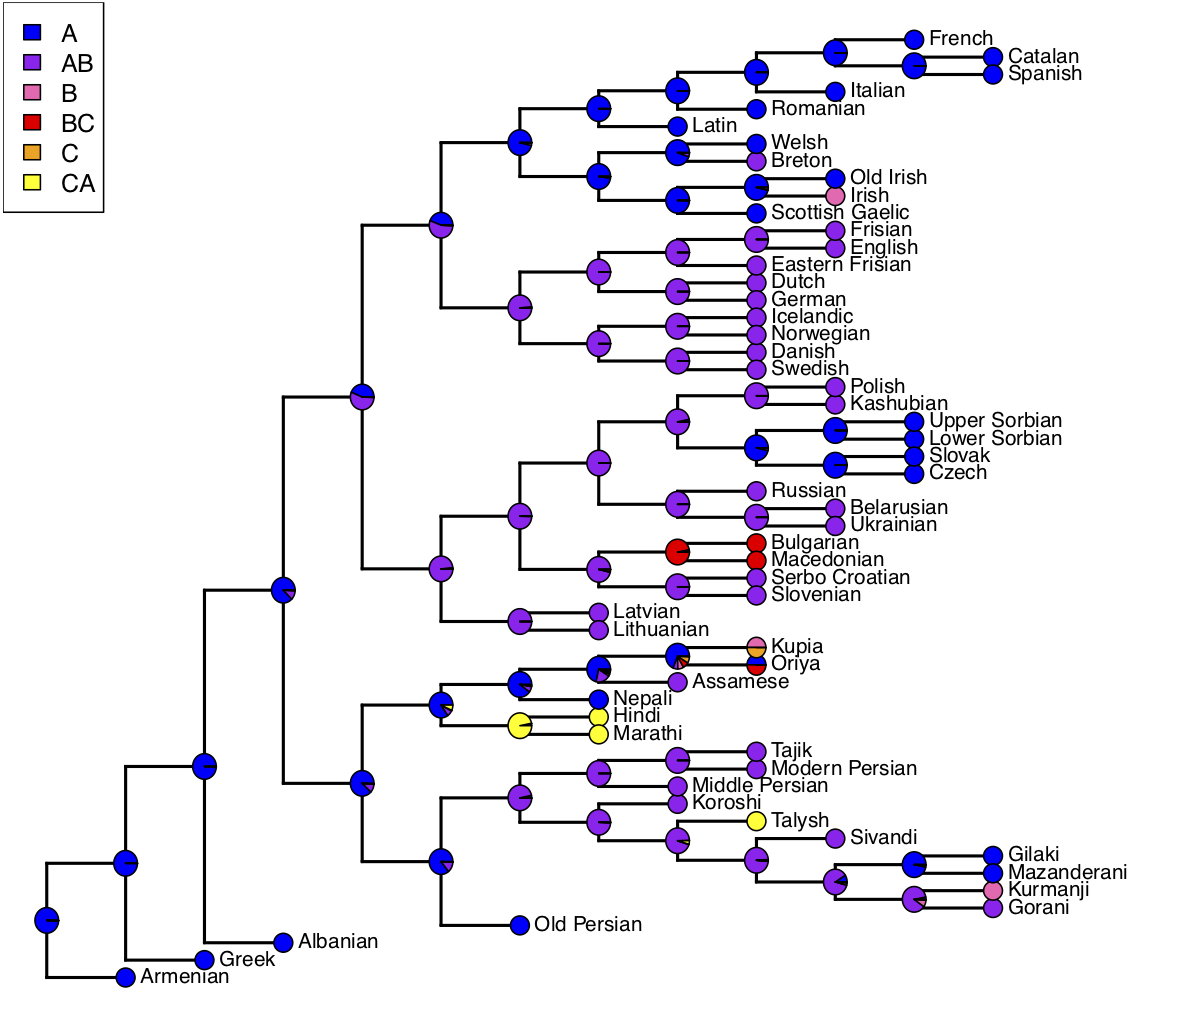
\includegraphics[width=\textwidth]{figures/IEUR-tree-with-pies.jpg}
\end{figure}

There are three reasons why we choose to display the classifications of the negative existentials in our sample on a phylogenetic tree: 1) this format may provide us with an insight into the validity of the NEC; 2) it helps us to estimate the stability of certain classifications over time; and 3) it contributes to our ultimate aim of conducting a phylogenetic comparative analysis of a larger dataset. 

The first point is relevant, for example, for the status of Gilaki and
Mazanderani. They ``return'' to state A while their immediate ancestor, as most contemporary Iranian languages, was likely state A{\textasciitilde}B. This suggests an innovation and loss of type B constructions rather than a very rapid cycling through the NEC. This type of innovation can involve factors such as an emergent locative copula based on verbs such as `stay' or `be at'. These types of innovative copulas tend to retain verbal negation patterns, which results in a Type A negative existential construction. A loss of a Type B construction which co-exists with a Type A construction, then, might seem like a “return” to Type A from Type A{\textasciitilde}B. 

As for the second point, it is easy to use the format of the phylogenetic tree to determine the stability of some types over time. All the Romance languages investigated thus far, including Latin, are of type A.  If we add the time that each of these languages has been independent from its sister languages, that is, the time elapsed since two sister languages separated from their common ancestor, then Type A appears to be a stable trait of this subfamily for thousands of years of evolution. Of course, we have only investigated 6 languages out of 80 Romance varieties, so this is only a preliminary suggestion at best. 

A similar logic applies to the Germanic languages. Proto-Germanic reconstructs as state A{\textasciitilde}B in the current analysis. The data from the contemporary Germanic languages also suggest that Type B constructions, where negation is expressed by a negative quantifier, are quite old and were possibly a part of the Proto-Germanic inventory. Despite the variation in the usage of negative quantifiers in Type B constructions across the Germanic languages, these Type B constructions are 1) at least in part cognate terms and 2) relevant in the description of all the Germanic languages we examined thus far. 

Another example of a relatively stable pattern is the prevalence of Type
A({\textasciitilde}B) constructions across Iranian. In Iranian, the Past
tense copular verbs, which are cognates of Middle Persian \textit{būd}
`was', were often retained in negative existential clauses. The combination
of these copulas and the Iranian negative particle \textit{ne} did not
undergo reduction and univerbation, which was presumably also due to
phonotactic constraints (unlike the Present tense copulas, see
\sectref{sec:ieur-4.1} above). Consequently, the negative existential with the Iranian Past tense copula is negated by the same marker that is used to negate prototypical verbs. The result is a conservative Type A negative existential construction. The reduction of the Present tense copula and the Iranian Negative particle resulted in a Type B construction, which leads to the classification of many Iranian languages as instances of Type A{\textasciitilde}B. 

  The third point is that we argue that phylogenetic comparative analyses are suitable to formally analyze the results of the Negative Existential Cycle within a single family. Thus far, we have conducted preliminary phylogenetic comparative analyses on the current dataset to test whether Croft's NEC more adequately explains the attested cross-linguistic distribution of negative existential patterns than alternative models. The Negative Existential Cycle makes the following highly specific claim regarding the expected direction of changes in the negative existential domain: 

\begin{equation*}  
A > A{\textasciitilde}B > B > B{\textasciitilde}C > C > C{\textasciitilde}A > A
\end{equation*}
%
These directional changes can easily be contrasted with alternative models, such as the reverse pattern of change:
%
\begin{equation*}  
A < A{\textasciitilde}B < B < B{\textasciitilde}C < C < C{\textasciitilde}A < A
\end{equation*}
%
Comparing the likelihood of pathways of change is possible even if not all construction types are attested in the dataset. Nevertheless, our preliminary testing suggests that our dataset is too limited to answer this question. Together with \citegen{Veselinova2014} Slavic data, we have information on the negative existential constructions in 55 Indo-European languages. Yet for at least two groups, Romance and Germanic, our data is completely void of variation, and thus from an evolutionary perspective, the data are useless to determine which paths of change are likely and which are unlikely. Given the variation we discovered in Indo-Iranian languages, we aim to collect a larger dataset that includes many more languages of this subfamily, as well as additional Romance and Germanic languages. 

The lack of special negative existential markers or constructions in the
language families of Western Europe that was first noted by
\citet[117]{Veselinova2013} warrants further explanation, particularly now
that we have essentially replicated this finding by consulting a larger
language sample. First, the current dataset suggests that Type A is
ancestral to the Indo-European language family. This is a very tentative
conclusion – even though Albanian, Modern Greek, and Modern Armenian
represent subfamilies that split off from the Indo-European family first
\parencite[at least in][]{BouckaertLemey2012}, each has been evolving for
thousands of years and the different components attested in their negative
existential constructions are not always cognate. As a consequence, despite
their seeming uniformity, it is unclear at this point whether the ancestors
of these languages were also Type A. Another focus for a larger dataset
should thus be to collect data from a larger set of ancient languages.
However, for the time being, we must acknowledge that when addressing the
dominance of Type A in Western Europe, we are most likely discussing a
stable, inherited state \parencite[see][19]{Croft1991} and not a number of independent changes towards Type A. 

An explanation for the lack of special negative existential constructions
in Western Europe is likely to be dependent on the inheritance or expansion
of specific constructions, as noted by \citet[1330]{Veselinova2014} for
Slavic. The question is why the Romance languages, at least those featured
in the current paper, do not change to Type A{\textasciitilde}B given their
tentative ancestral Type A classification, while at least some Slavic and
most Indo-Iranian languages do.%
%
\footnote{It should be noted that spoken French is moving towards stage
A{\textasciitilde}B. The fixed expression \textit{il n’y
pas} `there is\slash are no' is essentially a phonologically reduced,
single lexical unit (p.c. Ljuba Veselinova).} 
%
And why do negators and verbs in Germanic not merge to form special
negative existential constructions? We suggest that an explanation must at
least partly involve the morpho-phonology of the standard negation marker.
\citet{Dryer2013} reports that the negation in the Indo-European languages
of Europe is marked by negative particles rather than negative affixes
(with few exceptions in Eastern Europe, including Lithuanian, Latvian,
Czech, and Sorbian). Presumably one of the most common pathways to Type
A{\textasciitilde}B, merging the negator with an existential verb, is less
likely due to the phonotactic, prosodic, and word order environments in the
Western European languages. The morphological distance between the standard
negation marker and the verb could therefore prohibit a reduction, which
would have then led to the emergence of Type A{\textasciitilde}B in Western
Europe. This is similar to the suggestion made above regarding the lack of
reduction of the negation marker and the Past tense copula in Iranian. We
do not posit the reluctance of a merger of the negation marker and the verb
as the only or even the most important factor. The frequent use of the
negative quantifier in Germanic may certainly likewise play a role. The
central position of the Germanic and Romance languages in the Standard
Average European Sprachbund \parencite{Auwera2011} may also have been significant in the stability of the Romance Type A construction and the Germanic specific Type A{\textasciitilde}B constructions. Recent work by \citet{Drinka2017} on perfect constructions also demonstrates the workings of areal influence in European languages.  

Our study also supports Veselinova's finding \citep[1343--1366]{Veselinova2014}, which was also noted by Croft, that some languages have two distinct negative existential construction types, each potentially belonging to a different stage of Croft's cycle. Our data includes some similar scenarios in the Indo-Iranian languages and to a lesser extent in the Germanic languages. Acknowledging that multiple types of negative existential constructions may co-exist in the same language necessitates that we reconsider: 1) which types of constructions \textit{do} co-exist, and which \textit{cannot} co-exist, and 2) when two construction types co-exist, what effects will a change to one construction have on the classification of the other, and will these effects be in the same direction as \citegen{Croft1991} cycle? That is, if a combination of construction types does not occur, can we therefore argue that it is because it cannot emerge during language change or is it because of how the different negative existential construction types are defined?

\citet{Veselinova2014} demonstrates in her Polynesian data that Type B constructions can co-exist with Type B{\textasciitilde}C constructions (as in Kapingamarangi), and that constructions of Type B can co-exist with constructions of Type C (as in Tahitian). We presented above the same patterns of co-existence in Kupia and Standard Oriya, which are both Eastern Indo-Aryan languages. Furthermore, nothing appears to prohibit a language from having multiple constructions of Type A (that is, two distinct negation markers, both also used to negate existential predicates), or multiple constructions of Type B (such as two special negative existential markers). 

There seems to be, however, some restrictions to the co-existence of Type C constructions and other types of constructions. First, it appears that two Type C constructions cannot co-exist. Such a situation would entail that two distinct negation markers be used both as negative existential predicates and to negate verbs (under some different conditions, presumably). By definition, in this context, some variation occurs in the expression of verbal negation. Each of the two negative existential markers, then, is used to negate verbs only under some conditions, which means that the two negative existential constructions should be classified as instances of Type B{\textasciitilde}C. Another combination which seems impossible is two non-cognate constructions of Type A and Type C. Again, this situation has two distinct (and potentially non-cognate) verbal negation markers, which means that the verbal negation marker which doubles as a negative existential marker is used to negate verbs only under some conditions, and hence should be classified as an instance of Type B{\textasciitilde}C. 

The logical impossibility of some combinations of the construction types
defined by \citet{Croft1991} and \citet{Veselinova2014} means that at least
in some scenarios where a language has two distinct negative existential
constructions, a change in one entails a change in the second as well. Such
a possibility was mentioned in \sectref{sec:ieur-4.1} above for languages
with a Type B and a Type C construction, such as Kupia or Tahitian. In
these languages, an extension of the Type B negative existential marker to
be used for verbal negation (such as Type B > Type B{\textasciitilde}C)
would lead to variation in verbal negation. Thus, the status of the older
Type C construction would move ``backwards'' on \citegen{Croft1991} cycle to be Type B{\textasciitilde}C (i.e., Type C > Type B{\textasciitilde}C). This would lead to two B{\textasciitilde}C type constructions co-existing in the same language. In this situation, in turn, neither construction can move into the domain of Type C constructions without a loss of the other. In other words, as long as both Type B{\textasciitilde}C constructions co-exist, there is some variation in the domain of verbal negation. Thus, only a loss of this variation, that is, a loss of one of the Type B{\textasciitilde}C construction, would lead to a change in the status of the other to a Type C construction.

\section{Conclusions}\label{sec:ieur-6}

This paper offers an overview of the constructions that express negative existential functions in 42 Indo-European languages, which combined with \citegen{Veselinova2014} analysis of Slavic languages, results in data for 55 Indo-European languages. While this constitutes a rather small sample, we hope to expand this number to create a larger sample that may be used to conduct a comprehensive phylogenetic comparative analysis. Thus far, we detected distinct patterns of variation, with the Romance languages uniformly classified as Type A, the Germanic languages as uniformly Type A{\textasciitilde}B, while the Indo-Iranian language family is far more varied and with further study, may resemble Polynesian in that it contains all six types of the Negative Existential Cycle. The reason for these patterns of variation may be different patterns of morphosyntax and morpho-phonology in the different sub-branches of Indo-European, a hypothesis that would need to be tested in future work. We concluded by discussing the theoretical considerations that emerge when languages need to be classified as having two distinct negative existential constructions, when each may belong to a different type of the NEC. How these distinct negative existential constructions may interact has consequences for the expected diachronic changes within the Cycle. Hence, describing how negative existentials and standard negation interact has yet again become slightly more complicated, which is a good sign for the prospective study on this topic.\il{Indo-European|)}

\nocite{Schmitt1991}
\nocite{Shaked1979}
\nocite{Vahman1988}
\nocite{Williams1990}
{\sloppy
\printbibliography[heading=subbibliography,keyword=source,title={Sources}]
}

\section*{Acknowledgements}

We would like to thank Ljuba Veselinova first and foremost for getting us involved in negative existentials, believing that an analysis of Indo-European languages would be worthwhile, and for several rounds of feedback on earlier versions of this paper. We are also grateful for the helpful and challenging questions posed by an anonymous reviewer. We wish to express our appreciation to all those named below as well as unnamed who answered questions regarding the behavior of negative existentials in their languages of expertise. Special thanks to Cormac Anderson for his interest in this project.

\section*{Appendix A}

\textit{The translation questionnaire that was used to elicit data for many
languages in the current sample}

\subsection*{Negation questionnaire}

\begin{unindented}
The context descriptions are given in square brackets; further clarifications about the example sentences come in between parentheses. Neither the contexts, nor the clarifications are to be translated. Please translate only the \textbf{bold face text}. 

Please provide a morpheme to morpheme translation for all of the translated examples below. Should it turn out that the English examples/situations are in any way culturally inappropriate, e.g. take up topics or objects that are taboo or simply do not exist in your culture/language, feel free to substitute them with sentences that fit better your language. 

\textit{1. Language info}

\textit{1.1. Language name}

\textit{1.2. Genealogical affiliation}

\textit{1.3. Where is it spoken? Or where did you study it?}

\textit{2. Are you a native speaker? If not, how did you gain knowledge of
this language?}

\textit{3. Verbal sentences} 

(1) Example \\
\textbf{Mary sings} 

(2) Example \\
\textbf{Mary does not sing} 

(3) Example \\
\textbf{Mary likes movies} 

(4) Example \\
\textbf{Mary does not like movies} 

The answers to 3.1 below and sub-questions can be very short or just
references to other sources. 

3.1. Can you think of any tense-aspect categories where the negator used
in 1 through 4 cannot be used? If `yes':\\
3.1.1. Please name these categories. It would be helpful to give examples
too if possible (a pointer would be fine too, see above); \\
3.1.1.1. What negator is used with them? Again, examples or references are
welcome. 

\textit{4. Non-verbal sentences} 

\textit{4.1. Equational predicates}

(5) Example\\
{}[Introducing a guest to the family]: \textbf{This is my friend Tom}

(6) Example\\
{}[A family gathering plus a guest]\\
Your mom [looking at the guest]: Is this Tom?\\
Speaker B: \textbf{This is not Tom, it's Jake.}

\textit{4.2. Descriptive (property ascribing) predicates}

(7) Example\\
{}[Two people who met recently are talking about a common acquaintance]
Speaker A: What does Tom do?\\
Speaker B: \textbf{Tom is a teacher.}

(8) Example\\
{}[Same context as in (7)]\\
Speaker A: Is Tom a teacher?\\
Speaker B: \textbf{Tom is not a teacher, he is a doctor.}

(9) Example\\
{}[Talking about the appearance of a somebody I just met] \textbf{Tom is
tall.}

(10) Example\\
{}[Same context as in (9)] \textbf{Tom is not tall.}

(11) Example\\
{}[Tom just heard some really good news] \textbf{Tom is happy.}

(12) Example\\
{}[Tom is waiting for some news that's long delayed] \textbf{Tom is not
happy.}

\textit{4.3. Locative and locative-presentative predicates} 

(13) Example
{}[Somebody comes to your house, looking for your brother] (Yes, wait a
minute), \textbf{Tom/he is here.} 

(14) Example
{}[Same context as in (13)] (Sorry), \textbf{Tom/he is not
here.} 

(15) Example
{}[Same context as in (13)] (Sorry), \textbf{Tom/he is not
here, he is in town.} 

(16) Example
{}[Hearing trashing and noise, looking through the window] \textbf{There
are some wild cats in the garden.} 

(17) Example
{}[Same context as in (16)] Speaker A: Do you think there are
any wild cats in the garden? Speaker B: \textbf{There aren’t any wild cats
in the garden}. 

\textit{4.4. Clauses where only existence is predicated} 

(18) Example [The teacher, in a zoology/natural sciences class]
\textbf{There are wild cats} (in Africa or somewhere else; there is such a
thing as wild cats). 

(19) Example [Same context as in (18)] \textbf{There are no
wild cats} (in Africa or anywhere, there is no such thing as wild cats). 

(20) Example [Same context as in (18)] \textbf{Wild cats exist} (The sense
is the same as for 4.15; this is basically to check whether the language
has an intransitive existential verb as the English \textit{exist}, French
\textit{exister}, Modern Greek \textit{ipárho}, Russian
\textit{sushtestvovat’}.) 

(21) Example [Same context as in (18)] \textbf{Wild cats do not exist.} 

\textit{4.5 Predicative possession}

(22) Example\\
{}[Talking about helping somebody to move]\\
(Tom can help), \textbf{Tom/he has a car.}

(23) Example\\
{}[Same context as in (22)]\\
(Tom cannot help), \textbf{Tom/he does not have a car.}
\end{unindented}

\section*{Appendix B}\label{AppendixB}

\begin{unindented}
\textit{1. Indo-Iranian}

\textbf{Old} \textbf{Persian} (based on \citealt{Skjærvø2009b} and Bisitun inscription, \citealt{Schmitt1991})

Verbal negation: Preverbal \textit{naiy-}

Affirmative existential: the copular verb expresses existence (Skjærvø 2009b:134).

Negative existential: consists of a combination of the verbal negation
marker and the affirmative existential.
%
\begin{exe}\ex
    \gll naiy āha martiya   naiy  pārsa   naiy māda … \\
\textsc{neg} \textsc{cop.pst.3sg} man \textsc{neg} persian  \textsc{neg} median \\
    \glt `There was no man, not Persian, not Median, (… who dared to speak up).' (DB1:48--49)
    \end{exe}
%
\textbf{Summary: A}

\textbf{Middle Persian} (editions of primary texts used in the paper are cited above; see also Skjærvø 2009a for overview of Western Middle Iranian). 

Verbal negation: preverbal \textit{ne-} / \textit{nē-} (different philologists have different interpretations of the vowel length). 

Affirmative existential: expressed by clauses with a copular verb: \textit{būd-} for past and \textit{ast} for present.

Negative existential: with a past tense copula and its present tense counterpart \textit{baw-}, the standard verbal negation marker \textit{nē-} is found.
%
\begin{exe}\ex
    \gll agar ātaxš ī        wahrām  nē     būd \\
if      fire    \textsc{lnk}   Wahram \textsc{neg}  be.\textsc{pst.3sg} \\
    \glt `If the fire of Wahram did not exist (lit. if there was no fire of Wahram)'(PRDD:18)
    \end{exe}

The form \textit{ast} is negated by \textit{nēst} (or \textit{nest}; depending on vowel length interpretation). This negation marker is clearly an amalgam of \textit{nē-} and \textit{ast}, but there are good reasons to consider it as a unique marker.
%
\begin{exe}\ex
    \gll az      padīdīgīh   rāh  ī        ō dušaxw nest \\
from repentance road \textsc{lnk}   to hell      \textsc{neg.cop} \\
    \glt `From repentance, there is no road to Hell.' (DK6:50)
    \end{exe}

\textbf{Summary:} with the past tense, the negative existential is expressed by the copula preceded by the standard verbal negation marker, \textbf{hence: Type A}. In the present tense, a specific negative form of the copula is used, \textit{nēst}, therefore \textbf{Type B.} \textbf{Hence: Type A{\textasciitilde}B}
%

\textbf{Sivandi} (Data from \citealt{Lecoq1979}) 

Standard verbal negation: preverbal \textit{na-}, \textit{ne-}, \textit{ney-} 

Affirmative existential: figure + (ground) + copular verb
%
\begin{exe}\ex
    \gll ye šāh-i bi \\
one  king-\textsc{indef}    be.\textsc{pst}.\textsc{3sg} \\
    \glt `There was a king.' \citep[107]{Lecoq1979}
\ex \gll ye   čašme-y      en \\
one  fountain-\textsc{indef}   be.\textsc{prs.3sg} \\
    \glt `There is a fountain.' \citep[127]{Lecoq1979}
    \end{exe}

\textbf{Negative existential:}

1. The locative verb \textit{dār-} `be located', `be.at', `have' + standard verbal negation marker
%
\begin{exe}\ex
    \gll ke   bār   na=dār-e \\
\textsc{comp}   grain  \textsc{neg}=be.at-\textsc{3sg} \\
    \glt `(He closed his windmill down) because there was no grain.' \citep[150]{Lecoq1979}
    \end{exe} 

2. The past tense copulas + the standard verbal negation marker:
%
\begin{exe}\ex
    \gll albatta      barqa=m          na=bi \\
evidently  electricity=\textsc{top} \textsc{neg}-be.\textsc{pst.3sg} \\
    \glt `(Someone lit a candle), evidently there was no electricity.' \citep[89]{Lecoq1979}
    \end{exe}
3. \textit{Nūnd}, a negative copula.
%
\begin{exe}\ex
    \gll Kasi dege  ba goft=eš    nūnd           \\
Someone other to say=\textsc{3sg}  \textsc{neg}.\textsc{cop}  \\
    \glt `No one else answered his appeals.' \citep[95]{Lecoq1979}
\ex \gll vāllāh, me    či      tū  das=em      nūnd \\
by.god  \textsc{1sg}   what in hand=\textsc{1sg}    \textsc{neg.cop} \\
    \glt `By God, there's nothing in my hand' \citep[150]{Lecoq1979}
\ex \gll xolāse hīč    goftegūi  az      pīrežen-e          nūnd \\
and.finally \textsc{neg}  question from  old.woman-\textsc{def}   \textsc{cop.neg} \\
    \glt `And at the end, there were no questions from the old woman.' \citep[108]{Lecoq1979}
    \end{exe}

\textbf{Summary:} with two existential copulas, the past tense copula and
the locative verb, are negated by the standard negation form.
\textbf{Hence: Type A}. The present tense negative existential is expressed
using a negative copula \textit{nūnd}. \textbf{Hence: Type B.}\\
\textbf{Hence: Type A{\textasciitilde}B.}

\textbf{New Persian / Tajik} (own knowledge; p.c. Cormac Anderson; see also
\citealt{Perry2005}, \citealt{WindfuhrPerry2009})

New Persian and Tajik exhibit remarkably similar behavior. Verbal negation in both is expressed by the preverbal \textit{ne-}, \textit{ni-}. 

The affirmative existential is expressed by a combination of the figure (NP), optional ground (PP, NP), and a copular verb:
%
\begin{exe}\ex
    \glll dar in ōtaq   do   panjere  hast    (New Persian) \\
dar in       xona  du   tireza     hast    (Tajik) \\
in    \textsc{dem}  room  two window \textsc{ex.3sg}\\
    \glt `There are two windows in this room.' \parencite[450]{WindfuhrPerry2009}
    \end{exe}

Negative existentials are formed by replacing the affirmative existential copula \textit{hast} with its negative counterpart \textit{nest:} 
%
\begin{exe}\ex
    \gll Dar  in       χona    tireza     nest \\
in     \textsc{dem}   house   window \textsc{neg.cop.prs.3sg} \\
    \glt `There are no windows in this house.' (Tajik, \citealt[202]{Perry2005}
    \end{exe}

Past tense copulas are negated by \textit{ne-}, \textit{ni}- in this construction. Furthermore, in New Persian, \textit{daʃtan} `have' is used in the negative existential as well.
%
\begin{exe}\ex
    \gll gurba-ye vaʃi  na-dar-ad \\
cat-\textsc{lnk}   wild \textsc{neg}-have-\textsc{3sg} \\
    \glt `There are no wild cats.' (p.c. Cormac Anderson)
    \end{exe}

\textbf{Summary: Type A{\textasciitilde}B}

\textbf{Gorani} (Data from \citealt{MahmoudveysiBailey2012}.)

Verbal negation: prefixed / procliticized \textit{ne}- / \textit{na}- /
\textit{niy}- \parencite[25]{MahmoudveysiBailey2012}

Affirmative existentials are expressed by a copular verb that is preceded by the figure argument (with an optional ground argument).
%
\begin{exe}\ex \gll ya   dāya    kaywānū ma-w-u \\
one mother old.lady  \textsc{ind}-be.\textsc{prs.3sg} \\
    \glt `There is an old lady.' \parencite[15]{MahmoudveysiBailey2012}
\ex \gll čünka    nwār-aka       hē \\
because cassette-\textsc{def}  exist.\textsc{3sg} \\
    \glt `because there are cassettes' \parencite[34]{MahmoudveysiBailey2012}
    \end{exe}

Negative existentials are formed by \textit{nīya} or \textit{naw} that
\citeauthor{MahmoudveysiBailey2012} interpret as a negative copula. 
%
\begin{exe}\ex
    \gll falā-ka-y mwāy ay     wā     nīya \\
farmer-\textsc{def}-?   \textsc{ind}.say.\textsc{prs}.\textsc{3sg}  well  wind  not.exist.\textsc{3sg} \\
    \glt `The farmer says: “Well, there's no wind.”'
\parencite[61]{MahmoudveysiBailey2012}
\ex \gll masan yā   barq         naw \\
for.example one electricity \textsc{neg.cop} \\
    \glt `(when,) For example, there is no electricity.'
\parencite[159]{MahmoudveysiBailey2012}
    \end{exe}

\textbf{Summary}: Type A{\textasciitilde}B.

\textbf{Gilaki} \parencite{RastorguevaKerimova2012}

Verbal negation is expressed by a preverbal \textit{ne-}, \textit{na-}, \textit{n-}. The exact form is determined by phonotactics. 

Affirmative existential:
%
\begin{exe}\ex \gll ustatər utɐɣ=ə xɐli nah-a \\
over.there  room=\textsc{lnk}  empty exist.\textsc{prs.3sg} \\
    \glt `Over there, there is an empty room.' \parencite[310]{RastorguevaKerimova2012}
\ex \gll ita   rɐ    nah-a \\
one road exist-\textsc{3sg} \\
    \glt `There is one road.' \parencite[318]{RastorguevaKerimova2012}
\ex \gll miz=ə=ru du=ta kitɐb dərə \\
table=\textsc{lnk}=on  two=\textsc{clf}   book be.located.\textsc{3sg} \\
    \glt `There are two books on the table.' \parencite[134]{RastorguevaKerimova2012}
\ex \gll ɐxər dín=u məzháb=u xudɐ ki is-ə \\
after.all religion=and faith=and   god   \textsc{comp}    be.\textsc{prs.3sg} \\
    \glt `After all, there is religion, faith and God.' \parencite[275]{RastorguevaKerimova2012} 
    \end{exe}

Negative existential: expressed by the verbal negation marker that is attached to one of the copulas used in the affirmative existential forms.
%
\begin{exe}\ex \gll u bəlɐyə ki dər dunyɐ nə-na bi \\
and misfortune \textsc{rel}  in   world \textsc{neg}-exist   be.\textsc{pst} \\
    \glt `whatever misfortune that existed in the world'\parencite[263]{RastorguevaKerimova2012}
\ex \gll mašin nə-ø-na-ø \\
car \textsc{neg}-\textsc{pfv}-exist.\textsc{pst-3sg.pst} \\
    \glt `There are no cars.' \parencite[326, their glosses and zeroes]{RastorguevaKerimova2012}
\ex \gll ame xɐnə   hitʃ   kəs n-es-ə \\
\textsc{1pl} house \textsc{neg} somebody \textsc{neg}-be.\textsc{prs-3sg}\\
    \glt `There is nobody at home.' \parencite[133]{RastorguevaKerimova2012} 
    \end{exe} 

\textbf{Summary}: Type A.

\textbf{Ziyarati} \citep{ShokriJahani2013} 

Verbal negation: expressed by \textit{ne-} or \textit{na-} prefix / proclitic.

Affirmative existential: expressed by the copular verb or by the locative copula \textit{dār}- `be.at' or `be located'.

\begin{exe}\ex \gll jānevar dar-e, xu    dar-e \\
wild.animals  be.at.\textsc{prs-3sg}   boar be.at.\textsc{prs-3s}g \\
    \glt `(Why (do) we need a night watchman?) There are wild animals; there are boars.' \parencite[84]{ShokriJahani2013}
\ex \gll messe alān  ye   jāmeā=i hasse ke … \\
for.example now  one shirt=\textsc{indef} be.\textsc{prs}.\textsc{3sg}    \textsc{comp} \\
    \glt `There is a shirt that (has buttons all the way up).'
\parencite[153]{ShokriJahani2013}
\ex \gll esā in rasmā ā-bee \\
nowadays \textsc{dem} ceremony-\textsc{pl} \textsc{prv}-be.\textsc{pst.3pl} \\
    \glt `Nowadays there are ceremonies …' \parencite[80]{ShokriJahani2013}
    \end{exe}

Negative existential: expressed by one of the copulas above preceded by a verbal negation marker.

\begin{exe}\ex \gll ʃupā da-ni-bu-in … \\
watchman \textsc{prv}-\textsc{neg}-be.\textsc{pst}-\textsc{3pl} \\
    \glt `(if) there are no watchmen' \parencite[84]{ShokriJahani2013}
\ex \gll ammā dige  age  na=bu ke … \\
but \textsc{prt} if \textsc{neg}=be.\textsc{pst}.\textsc{3sg} \textsc{comp}  … \\
    \glt `but if there is no one who (want to buy our goods)'
\parencite[82]{ShokriJahani2013}
\ex \gll zemestān o bāhār  o payiz o tābestān ne=dāʃt-e \\
winter and spring and autumn and summer \textsc{neg}-be.at.\textsc{pst-3sg}\\
    \glt `There was no winter, spring, autumn, and summer (i.e., where we live there is no difference between the seasons).' \parencite[65]{ShokriJahani2013}
    \end{exe} 

\textbf{Summary: Type A.}

\textbf{Kurmanji} (\citealt{Thackston2006}, our glosses and parsing)

Verbal negation: \textit{na}, \textit{ne}.\\
Affirmative existential: formed with the usual copulas preceded by a single figure constituent.
%
\begin{exe}\ex \gll Got-in-eke pêşiy-ên me heye.  \\
say-\textsc{nmz}-\textsc{indef}   ancestor-\textsc{pl} \textsc{1pl}.\textsc{obl}   be.\textsc{prs.3sg} \\
    \glt `There is a saying of our ancestors.' \parencite[31]{Thackston2006}
    \end{exe} 

Negative existential: expressed by \textit{tun-} 
%
\begin{exe}\ex \gll Di vî warî    da otorîtey-eke resmî   tune.  \\
in  \textsc{dem}    regard in  authority-\textsc{indef}  official \textsc{cop.neg.prs.3sg} \\
    \glt `In this regard, there is no official authority.' \citep[32]{Thackston2006}
\ex \gll Madem ku zimannivîs tune \\
as.long.as  \textsc{comp}    writer \textsc{cop.neg.prs.3sg} \\
    \glt `as long as there are no writers' \citep[32]{Thackston2006}
\ex \gll Ger xwendevan-ên kurdî tunebin \\
if reader-\textsc{pl} Kurdish  \textsc{cop.neg.pst} \\
    \glt `if there are not readers of Kurdish' \citep[31]{Thackston2006}
    \end{exe}

\textbf{Summary: Type B.}

\textbf{Taleshi} \parencite{Paul2011}. 

Verbal negation: The standard verbal negation is a \textit{nə-}, \textit{ni-}.

Affirmative existential:
%
\begin{exe}\ex
    \gll vind=əš=e də   gəla əmsafa hest-e \\
see=\textsc{3sg}=\textsc{trs} two \textsc{clf} then exist-\textsc{3sg} \\
    \glt `He saw that there are two baskets.' \citep[358]{Paul2011}
\ex \gll vin-ən kə bale, vâš    b-a \\
see-\textsc{3pl} \textsc{comp}     yes   grass be-\textsc{3sg} \\
    \glt `They see that yes, there's grass.' \citep[210]{Paul2011}
\ex \gll iâ rama=i dari=a \\
here flock=\textsc{indef} exist=\textsc{cop.3sg} \\
    \glt `There is a flock here.' \citep[243]{Paul2011}
    \end{exe}

Negative existential: The standard verbal negation is often used:
%
\begin{exe}\ex \gll ǧeir   az   xudâ hikas    ne-bu \\
apart  from  god   nobody \textsc{neg}-be.\textsc{3sg} \\
    \glt `Apart from God, there's nobody.' \citep[176]{Paul2011}
\ex \gll vin-ə sas=i ni=a \\
see-\textsc{3sg} voice=\textsc{indef}  \textsc{neg=cop.3sg} \\
    \glt `She sees that there is no answer.' \citep[422]{Paul2011}
    \end{exe}

Rarely in the data presented in \citealt{Paul2011} \textit{ni} is used alone in negative existentials:
%
\begin{exe}\ex
    \gll câra=i ni magam əm ki bə-š-am \\
solution=\textsc{indef} \textsc{neg} except \textsc{demp} \textsc{comp} \textsc{sujb}-go-\textsc{1pl} \\
    \glt `There is no solution but that we go.' \citep[214]{Paul2011}  
    \end{exe}

\textbf{Summary: Type C{\textasciitilde}A}

\textbf{Koroshi} \parencite{NourzaeiJahani2015}

Verbal negation: expressed by a preverbal \textit{na}-, \textit{nā}- \textit{nay}-.

Affirmative existential: expressed by the copula preceded by a single-figure constituent (and an optional ground constituent). 
%
\begin{exe}\ex \gll ye ādam=e bīčāra=en \\
one person=\textsc{lnk}   poor=\textsc{cop.npst.3sg} \\
    \glt `There is a poor fellow.' \parencite[31]{NourzaeiJahani2015}
\ex \gll yek dāzan=ē bod-a=ø \\
one woman=\textsc{indef} become.\textsc{pst-pp=cop.npst.3sg} \\
    \glt `There is (lit. has been) a woman.' \parencite[90]{NourzaeiJahani2015}
    \end{exe} 
%
Negative existential: expressed by a copula preceded by the verbal negation marker: 
%
\begin{exe}\ex \gll ġayr az xodā hīčka nay-at-Ø \\
except from god   nobody \textsc{neg-cop.pst-3sg} \\
    \glt `Except for God, there was no one.'
(\citealt[123]{NourzaeiJahani2015}; formula)
    \end{exe}
%
Occasionally found expressed by \textit{nē}, which is not mentioned in the grammar sketch by Nourzaei et al., but is glossed by them as a non-past tense copula.
%
\begin{exe}\ex \gll bāk=ē nē \\
fear=\textsc{indef}    \textsc{neg}.be.\textsc{npst.3sg} \\
    \glt `(And I said:) No problem!' \parencite[149]{NourzaeiJahani2015}
\ex \gll be.xātere.ke ay dar=ī fāyeda nē \\
because from in=\textsc{pc}.\textsc{3sg} use \textsc{neg}.be.\textsc{npst.3sg} \\
    \glt `because there was nothing to gain (lit. there is no use)'
\parencite[144]{NourzaeiJahani2015}
    \end{exe}

\textbf{Summary: A{\textasciitilde}B}

\textbf{Hindi} \parencite[see][]{Bashir2006}

\textbf{Odia} \parencite{NeukomPatnaik2003}

Verbal negation: The most common verbal negation marker is a post-verbal \textit{nahĩ}. The copula \textit{th-} (often referred to as a locative but used for other functions as well) is negated by a preverbal \textit{nɔ-} and this negative marker is occasionally also found on other, lexically heavy verbs. This occurs when an old \textit{th-} auxiliary is involved in the creation of the form, but it is also found in other circumstances.
%
\begin{exe}\ex \gll se gɔl-a nahĩ \\
\textsc{3sg}   go.\textsc{pst-3sg}  \textsc{neg} \\
    \glt `He did not go.' \parencite[340]{NeukomPatnaik2003}
\ex \gll se muɳɖɔ hɔla-i nahĩ kɔr-iba-ru ɔnyɔ jɔɳɔ-kɔ kɔh-il-a \\
\textsc{3sg} head shake-\textsc{cv} \textsc{neg} do-\textsc{inf-abl} other \textsc{clf-def} say-\textsc{pst-3sg} \\
    \glt `since she shook her head and said no, the other one
said…'\parencite[43]{NeukomPatnaik2003}
\ex \gll kheɭ-u-nɔ-th-il-a \\
play-\textsc{ipfv-neg-aux-pst-1sg} \\
    \glt `I was not playing.' \parencite[340]{NeukomPatnaik2003}
\ex \gll kintu bɔrttɔman se nɔ-j-ib-ɔ kahĩki \\
but now \textsc{3sg} \textsc{neg}-go-\textsc{fut-3sg} why \\
    \glt `But why shouldn't she go now?’ \parencite[341]{NeukomPatnaik2003}
\ex \gll ta-ku sɔtɔrkɔ kɔr-a-i-de-b-e puɔ jemiti istri nɔ-chũ-ẽ\\
\textsc{3msg-dat} careful do-\textsc{caus-cv}-give-\textsc{fut-2pl} boy in.order iron \textsc{neg}-touch-\textsc{3sg.hab} \\
    \glt `Warn her that the boy should not touch the iron.' \parencite[155]{NeukomPatnaik2003}
    \end{exe}
%
Affirmative existential: The usual verbal copulas \textit{ɔch-} and \textit{th-} are used here.
%
\begin{exe}\ex \gll eʈhi kete-guɽie  saikel  ɔch-i   \\
here some-\textsc{pl}  bicycle be-\textsc{3sg} \\
    \glt `There are some bicycles here.' \parencite[47]{NeukomPatnaik2003}
\ex \gll tumɔ laibreri-re bɔngɔɭa bɔhi  ɔch-i? hɔ̃ kete-khɔɳɖɔ ɔch-i \\
\textsc{2sg} library-\textsc{loc} Bangla book be-\textsc{3sg} yes some-\textsc{clf} be-\textsc{3sg} \\
    \glt `Are there Bengali books in your library? Yes, there are some.'
\parencite[118]{NeukomPatnaik2003}
\ex \gll e bɔs-re purusɔ o stri-manɔ-nkɔ-rɔ bɔs-iba jaga  ɔch-i \\
\textsc{dem} bus-\textsc{loc} man and woman-\textsc{pl-obl-gen} sit-\textsc{inf} place be-\textsc{3sg} \\
\glt `In this bus there are seats for gentlemen and (seats) for ladies.'
\parencite[38]{NeukomPatnaik2003}
    \end{exe}

Negative existential: The post-verbal negation marker \textit{nahĩ} is used without a copula (B{\textasciitilde}C, because there is another SN). Neukom and Patnaik parse this marker as a negative copula and a third person singular bound person marker. As \textit{th-} is negated with a preverbal \textit{nɔ-}, it is also negated in this manner when it functions as the existential copula. This negation marker is also used with prototypical action verbs (not only when \textit{th-} is an auxiliary). 
%
\begin{exe}\ex \gll deuɭɔ bhitɔr-e kie ɔch-i ki? na, kehi nah-ĩ \\
temple inside-\textsc{loc}   someone be-\textsc{3sg}   \textsc{int}      no  anyone \textsc{neg}.be-\textsc{3sg} \\
    \glt `Is there someone in the temple? No, there isn't anyone.'
\parencite[100]{NeukomPatnaik2003}
\ex \gll bɔɽɔ nah-ĩ choʈɔ di-ɔ \\
big \textsc{neg}.be-\textsc{3sg} small give-\textsc{2pl.impr} \\
    \glt `There are no big (ones); give me small (ones).' \parencite[72]{NeukomPatnaik2003} 
\ex \gll premika nɔ-th-ile birɔhɔ jɔntrɔɳo nɔ-tha-nt-a ki kehi mɔdɔ pi-u-nɔ-tha-nt-e \\
mistress \textsc{neg}-be-\textsc{cond}.\textsc{cv}   separation pain        \textsc{neg}-be-\textsc{cond}-\textsc{3sg} or anybody wine drink-\textsc{ipfv-neg-aux-cond-3pl} \\
    \glt `If there were no girls, there would be no pain of separation nor
would anybody drink alcohol.' \parencite[195]{NeukomPatnaik2003}
\end{exe}

\textbf{Summary: Type A \& Type B{\textasciitilde}C} 

\textbf{Nepali} (p.c. Sugam Singh, with the help of Marie-Caroline Pons)

Verbal negation: -\textit{dina} and \textit{-in}(\textit{a})\textit{n} verbal suffixes; both can be further parsed, but this is not essential to illustrate the point here.
%
\begin{exe}\ex \gll yini mahilã git gãũ-dina-n \\
\textsc{dem}   woman song sing-\textsc{neg.prs.3sg} \\
    \glt `The woman doesn't sing.' (p.c. Sugam Singh)
\ex \gll yini mahilã-le git gã-inan \\
\textsc{dem} woman-\textsc{erg} song sing-\textsc{neg.pst.3sg} \\
    \glt `The woman didn't sing.' (p.c. Sugam Singh)
\ex \gll yini mahilã jhyal phoɖ-dinan \\
\textsc{dem} woman window break-\textsc{neg.prs.3sg} \\
    \glt `The woman didn't break the window.' (p.c. Sugam Singh)
\ex \gll yini mahilã-le jhyãl phoɖ-inan \\
\textsc{dem}   woman-\textsc{erg}  window break-\textsc{neg.pst.3sg} \\
    \glt `The woman didn't break the window.' (p.c. Sugam Singh)
\end{exe}

Affirmative existential: with the usual verbal copulas. 
%
\begin{exe}\ex \gll bāri-mã birālo-haru chha-n \\
garden-\textsc{loc} cat-\textsc{pl} be-\textsc{3sg} \\
    \glt `(When he looked outside) there were cats in the garden.' (p.c. Sugam Singh)
\ex \gll bāri-mã birālo-haru thi-e \\
garden-\textsc{loc} cat-\textsc{pl} be.\textsc{pst-3sg} \\
    \glt `(When he looked) there were no cats in the garden.' (p.c. Sugam Singh)
    \end{exe}

Negative existential: The usual verbal negation markers are used here regardless of tense/aspect.
%
\begin{exe}\ex \gll bāri-mã birālo-haru  chha-inan \\
garden-\textsc{loc} cat-\textsc{pl} be-\textsc{neg.prs.3sg} \\
    \glt `(He is looking outside) There at no cats in the garden.' (p.c. Sugam Singh)
\ex \gll bāri-mã birālo-haru  thi-enan \\
garden-\textsc{loc} cat-\textsc{pl} be-\textsc{neg.pst.3sg} \\
    \glt `(he looked outside) There were no cats in the garden.' (p.c. Sugam Singh)
\ex \gll jãgali birālo-haru hũ-deinan \\
jungle cat-\textsc{pl} be.\textsc{prs-neg.prs.3sg} \\
    \glt `There are no wild cats' (also given for `wild cats don't exist’). (p.c. Sugam Singh)
\ex \gll jãgali birālo-haru thi-enan \\
jungle cat-\textsc{pl} be.\textsc{pst-neg.pst.3sg} \\
    \glt `There were no wild cats (back in the day, before they were brought here).' (p.c. Sugam Singh)
    \end{exe} 

\textbf{Summary: Type A.}

\textbf{Assamese} (p.c. Krishna Boro and Nihankara Dutta).

Verbal negation: Verbs are negated by a \textit{ni-} prefix or by a
\textit{nasil} negative auxiliary. The negative auxiliary is probably
historically \textit{ni-} + \textit{as} \textsc{cop} + \textit{il}
\textsc{pst}, and are parsed here in this manner. Whether this parsing is a synchronic reality in the minds of speakers is questionable (we would like to thank Krishna Boro for this point).
%
\begin{exe}\ex \gll Mohila-goraki{\op}-e{\cp} gan na-ga-j \\
Woman-\textsc{clf(-nom)}  song \textsc{neg}-sing-\textsc{3sg} \\
    \glt `The woman didn't sing.' (p.c. Krishna Boro and Nihaikara Dutta)
\\
(some experts consider the optional –e an Ergative marker)
\ex \gll mohila-goraki{\op}-e{\cp} gan  go-a n-as-il-e \\
woman-\textsc{clf}(-\textsc{nom}) song sing-\textsc{ptcp} \textsc{neg-cop-pst-3sg} \\
    \glt `The woman didn't sing.' (p.c. Krishna Boro and Nihaikara Dutta)
    \end{exe}

Affirmative existential: The usual verbal copulas \textit{as-} or \textit{tʰak-} are used here. The later is often referred to as a “locative” existential in the (Eastern) Indo-Aryan literature, but it can be found also in other types of nominal predication domains.
%
\begin{exe}\ex \gll sotal-ot keitaman mekuri as-e \\
yard-\textsc{loc}  some cat \textsc{cop-3sg.prs} \\
    \glt `(Hearing noise from outside) there are some cats in the yard' (p.c. Krishna Boro and Nihaikara Dutta)
\ex \gll sotal-ot keitaman mekuri as-il \\
yard-\textsc{loc} some cat \textsc{cop-pst} \\
    \glt `(When he looked to the yard) there were some cats in the yard.' (p.c. Krishna Boro and Nihaikara Dutta)
\ex \gll bonoria mekuri tʰak-e / as-e \\
wild cat stay-\textsc{3sg.prs} / \textsc{cop-3sg.prs} \\
    \glt `There are wild cats.' (p.c. Krishna Boro and Nihaikara Dutta)
    \end{exe}

Negative existential: A special negative existential \textit{nai} is used
(hence: Type B), but also \textit{na-} and \textit{nasil} are found (hence
Type A). There seems to be a tense\slash aspect interaction with regards to the distribution of these markers.
%
\begin{exe}\ex \gll sotal-ot {\op}eta-u{\cp} mekuri nai \\
yard-\textsc{loc} (one-\textsc{add}) cat \textsc{neg.ex} \\
    \glt `(He's looking into the yard) there are no cats in the yard.' (p.c. Krishna Boro and Nihaikara Dutta)
\ex \gll sotal-ot {\op}eta-u{\cp} mekuri  n-as-il \\
yard-\textsc{loc} one-\textsc{add} cat \textsc{neg}-be-\textsc{pst} \\
    \glt `(When he looked into the yard) there were no wild cats in the yard.' (p.c. Krishna Boro and Nihaikara Dutta)
\ex \gll bonoria mekuri na-tʰak-e \\
wild cat \textsc{neg}-stay-\textsc{3sg} \\
    \glt `There are no wild cats.' (p.c. Krishna Boro and Nihaikara Dutta) (the verb in this clause means `stay, be at, exist')
\ex \gll bonoria mekuri n-as-il \\
wild cat \textsc{neg}-be-\textsc{pst} \\
    \glt `There were no wild cats (back in the day, before they were brought here).' (p.c. Krishna Boro and Nihaikara Dutta)
    \end{exe}

\textbf{Summary: Type A{\textasciitilde}B}

\textbf{Kupia} (\cites{Christmas1973a}{Christmas1973b}; we will not repeat examples from the paper here)

Verbal negation: Is expressed by a post verbal \textit{nay} (see the example in our article). 

Affirmative existential: Copular verb + NP expressing the figure + optional NP / PP expressing the ground.

Negative existential: There are two construction types. In both, the copula is replaced completely by a different marker. Construction type one is of type B, and a special negative form of the copula (\textit{nenj-}) replaces the copular verb used in the affirmative. The second is of type C and the Verbal negation marker is used as a special negative existential marker.

\textbf{Summary: Type B and Type C.}\\

\textit{2. Albanian, Armenian, Greek}

\textbf{Albanian}

Standard (Tosk) Albanian has four negative morphemes, \textit{nuk},
\textit{s’}, \textit{mos} and \textit{jo} \citep[82]{Turano2000}, see
\citet[172]{BuchholzFiedler1987} for another negative morpheme,
\textit{as}. \textit{mos} is used to negate subjunctive, imperative and
optative clauses as well as gerunds and infinitives \citep[85]{Turano2000}.
\textit{jo} often referred to as a `constituent negator' and is restricted
to use with nominals, adjectives, prepositional phrases, and adverbials
\citep[86]{Turano2000}. Only \textit{nuk} and \textit{s’} are relevant for
the present discussion. They are interchangeable even though they are used
differently \parencite[172]{BuchholzFiedler1987}. Both occur in standard negation:
%
\begin{exe}\ex \gll Nuk vajta (më) në bibliotekë.  \\
\textsc{neg} go.\textsc{pst.1sg} (anymore) in library \\
    \glt `I didn't go to the library (anymore).' \citep[82]{Turano2000}
\ex \gll S’-vajta (më) në bibliotekë.  \\
\textsc{neg}-go.\textsc{pst}.\textsc{1sg} (anymore) in library \\
    \glt `I didn't go to the library (anymore).' \citep[82]{Turano2000}
    \end{exe}

The verb used for existential predicates is \textit{ka} `to have', as
indicated by \citet[12]{Camaj1984}, who explicitly glosses the third person
singular form of the verb, \textit{ka}, to mean `he, she has; there is',
and its negated form is \textit{nuk ka}, \textit{s’ka} with `there is no'. 

\citegen{Camaj1984} grammar includes several examples of existential predicates. The examples below illustrate the use of the affirmative and negated existential predicates:
%
\begin{exe}\ex \gll Në mulli ka drithë e miell \\
in mill have.\textsc{3sg} grain and flour \\
    \glt `In the mill there is grain and flour.' \parencite[12/257]{Camaj1984}
\ex \gll ndër ne s’ka kundërshtime \\
among \textsc{1pl}.\textsc{acc} \textsc{neg}+have.\textsc{3sg} objection.\textsc{pl} \\
    \glt `There are no conflicts among us.' \citep[70]{Camaj1984}
    \end{exe} 

As \textit{ka} `to have' is negated as any other verb, Albanian is classified as a type A language. 

\textbf{Armenian}

Modern (Eastern) Armenian has the negative prefix \textit{čʻ-} for standard
negation and this prefix attaches to most verb forms, except for
imperatives \parencite[522]{DumTragut2009}:
%
\begin{exe}\ex \gll Vardan-ě gnecʻ gírkʻ-ě.  \\
Vardan.\textsc{nom}-\textsc{def} buy.\textsc{aor}.\textsc{3sg} book.\textsc{nom-def} \\
    \glt `Vardan bought the book.' \parencite[51]{DumTragut2009}
\ex \gll Vardan-ě čʻ-gnec’ gírkʻ-ě.  \\
Vardan.\textsc{nom}-\textsc{def} \textsc{neg}-buy.\textsc{aor}.\textsc{3sg} book.\textsc{nom-def} \\
    \glt `Vardan did not buy the book.' \parencite[51]{DumTragut2009}
    \end{exe} 

Modern Armenian \textit{em} `to be' expresses copular meaning and also
functions as an auxiliary \parencite[215]{DumTragut2009}:

\begin{exe}\ex \gll Anuš-ě gełecʻik   ałǰik ē. \\
Anuš.\textsc{nom}-\textsc{def} beautiful girl.\textsc{nom} is.\textsc{3sg} \\
    \glt `Anuš is a beautiful girl.' \parencite[215]{DumTragut2009}
\ex \gll Anuš-ě gełecʻik ałǰik čʻ-ē.  \\
Anuš.\textsc{nom}-\textsc{def} beautiful girl.\textsc{nom} \textsc{neg}-is.\textsc{3sg} \\
    \glt `Anuš is not a beautiful girl.' \parencite[215]{DumTragut2009}
    \end{exe}

The copula is used for locatives in the following:
%
\begin{exe}\ex \gll Im hayr-ě Ani hyuranocʻ-um ē.  \\
my father.\textsc{nom}-\textsc{def} Ani.\textsc{nom} hotel-\textsc{loc} be.\textsc{3sg} \\
    \glt `My father is in the Hotel Ani.' \parencite[382]{DumTragut2009}
    \end{exe}

However, another verb that is frequently used for both locative and true
existentials is the defective verb \textit{kam} `to exist' \parencite[282]{DumTragut2009}. The following are examples of a locative existential and a true existential:
%
\begin{exe}\ex \gll hamaynkʻ-i łekavar-i t-an-ě heṙaxos čʻ-ka.  \\
community-\textsc{dat} leader-\textsc{dat} house-\textsc{dat-def} 
telephone.\textsc{nom} \textsc{neg}-exist-\textsc{prs.3sg} \\
    \glt `There is no telephone in the house of the leader of the
community.' \\
\hspace{\stretch{1}}\parencite[104--105]{DumTragut2009}
\ex \gll inč’u čʻ-k-an barjrakarg ēkʻskursavar-ner?  \\
why \textsc{neg}-exist-\textsc{prs.3pl} high.quality tourist.guide-\textsc{pl.nom} \\
    \glt `Why there are no high-quality tourist guides?' (headline)
\parencite[693]{DumTragut2009}
    \end{exe}

It seems that both \textit{kam} `to exist' and the copula \textit{em} are used for locatives, while only \textit{kam} alone can be used to predicate existence, without reference to a specific situation or location. Both \textit{kam} and \textit{em} are negated with the negative prefix \textit{č’-}, classifying Modern Armenian as a type A language. 

\textbf{Modern Greek}

In Modern Greek\il{Modern Greek}, the negative morpheme δεν
(\textit{den}) `not' is placed before the verb to form a negative
indicative statement \parencite[510]{HoltonMackridge2012}. Another negator exists for sentences in the subjunctive mood, but this is not addressed here. 
%
\begin{exe}\ex \glll
Οι συγγενείς του δεν θα του δώσουν καμιά βοήθεια \\
\textit{Oi} \textit{syngeneís} \textit{tou} \textit{ðen} \textit{θa} \textit{tou} \textit{ðósoun} \textit{kamiá} \textit{voíθeia}\\
\textsc{def.pl}  relative.\textsc{pl} \textsc{poss.3sg} \textsc{neg}  \textsc{fut} \textsc{3sg.acc} give any aid \\
    \glt `His relatives are not going to give him any help.' \parencite[510]{HoltonMackridge2012}
    \end{exe}

It is possible to use the δεν (\textit{den}) `not' in combination with the
copula είμαι (\textit{eímai}) for many non-verbal predicates, including locatives:
%
\begin{exe}\ex \glll
Δεν είναι καμιά αδέσποτη γάτα στον κήπο \\
\textit{ðen} \textit{eínai} \textit{kamiá} \textit{aðéspoti} \textit{gáta} \textit{ston} \textit{kípo}\\
\textsc{neg} be.\textsc{3sg} none stray cat in.\textsc{def} garden \\
\glt `There isn't any wild cat in the garden.' (p.c. Eirini Skourtanioti)
    \end{exe}

Nonetheless, for existential predicates, υπάρχω (\textit{ypárcho}) `to
exist' or έχω (\textit{écho}) `to have' must be used rather than the copula:
%
\begin{exe}\ex \glll
Δεν υπάρχει φάρμακο σ'αυτή την αρρώστια \\
\textit{ðen} \textit{ypárchei} \textit{fármako} \textit{s’-aftí}
\textit{tin} \textit{arróstia} \\
\textsc{neg} exist medicine of-\textsc{dem.fsg} \textsc{def.acc} illness\\
    \glt `There is no cure [lit. ‘medicine'] for this illness.'
\parencite[493]{HoltonMackridge2012}
\ex \textit{Στην Ολλανδια, με νόμο του 1976 απαγορεύεται να ανοίγουν τα
καταστήματα τις Κυριακές, \ldots}\\
\glll
\ldots{}ενώ αντιθέτως στην Πολωνια δεν υπάρχουν πλέον περιορισμοί. \\
\ldots{}enó antiθétos stin Polonia ðen ypárchoun pléon periorismoí. \\
while instead in.\textsc{def} Poland \textsc{neg} exist much
restriction.\textsc{pl}\\
    \glt `In the Netherlands, a 1976 law prohibited opening shops on Sundays, whereas in Poland, there are no such restrictions anymore.' \citep[483]{Puigdollers2015}
\ex \glll
Δεν εχει φωτα στο σπιτι τους.  \\
\textit{ðen} \textit{echei} \textit{fota} \textit{sto} \textit{spiti} \textit{tous}.  \\
\textsc{neg} have.\textsc{prs.3sg} light.\textsc{pl} on.\textsc{def} house
\textsc{poss.3pl}\\
    \glt `There are no lights in their house.' \parencite[199]{HoltonMackridge2004}
\ex \glll
Δεν έχει αδέσποτες γάτες\\
\textit{ðen} \textit{échei} \textit{aðéspotes} \textit{gátes}\\
\textsc{neg}  have.\textsc{prs.3sg} stray cat.\textsc{pl} \\
    \glt `There are no stray cats.' (p.c. Eirini Skourtanioti)
    \end{exe}

While the copula cannot be used, Modern Greek is a clear instance of Type A
because it uses the standard negator for negative existentials. For a
similar analysis of Modern Greek, see also
\citet[115--116]{Veselinova2013}.  For more information regarding
diachronic change in Greek negation, see \citet{KiparskyCondoravdi2006-ieur}. 

\textit{3. Baltic}

\textbf{Latvian}

Standard negation in Latvian is expressed through the preverbal particle \textit{ne}: 
%
\begin{exe}\ex \gll Marija dzied \\
Mary sing.\textsc{prs.3sg} \\
    \glt `Mary sings.' (p.c. Sandra Grinberga)
\ex \gll Marija   ne   dzied \\
Mary \textsc{neg} sing.\textsc{prs.3sg} \\
    \glt `Mary does not sing.' (p.c. Sandra Grinberga)
\ex \gll Viņš ne-runā latviski \\
\textsc{3sg}.\textsc{masc} \textsc{neg}-speak.\textsc{prs.3sg} Latvian \\
    \glt `He doesn't speak Latvian.' \citep[164]{Mathiassen1997}
    \end{exe}

In negative existentials, as in many other contexts where the copula is used, the negated form of the copula \textit{ir} `to be' in the present tense has the form \textit{nav}: 
%
\begin{exe}\ex \gll Afrikā ir lauvas \\
Africa \textsc{cop} lion.\textsc{pl.nom} \\
    \glt `In Africa there are lions.' \citep[164]{Mathiassen1997}
\ex \gll Latvijā nav lauvu \\
Latvia \textsc{neg.cop} lion.\textsc{pl.gen} \\
    \glt `In Latvia there are no lions.' \citep[164]{Mathiassen1997}
\ex\begin{xlist}
\ex \gll Ir savvaļas kaķi \\
\textsc{cop} wild cat.\textsc{pl.nom} \\
    \glt `There are wild cats.' (p.c. Sandra Grinberga)
\ex\gll Nav savvaļas kaķu\\
\textsc{neg}.\textsc{cop} wild cat.\textsc{pl.gen}\\
\glt `There are no wild cats.' (p.c. Sandra Grinberga)
    \end{xlist}\end{exe}

In contrast, in the past tense, a regularly negated form of the copula is used:
%
\begin{exe}\ex \begin{xlist}
\ex\gll Bija savvaļas kaķi \\
\textsc{pst.cop} wild cat.\textsc{pl.nom} \\
    \glt `There were wild cats.' (p.c. Sandra Grinberga)
\ex\gll Ne-bija savvaļas kaķu\\
\textsc{neg}-pst.\textsc{cop} wild cat.pl.gen\\
\glt `There were no wild cats.' (p.c. Sandra Grinberga)
    \end{xlist}\end{exe}

The copula \textit{ir} `to be' is used in this manner for all the non-verbal sentences we investigated in our questionnaire, including equational predicates, descriptive predicates, locative predicates (see above, examples 96 and 97), and negative existentials. Hence, we classify Latvian as Type A{\textasciitilde}B, as a special negative existential construction exists but its usage is dependent on TAM. 

\textbf{Lithuanian}

\citet[176--177]{Mathiassen1996} states that the most important verbal negator in Lithuanian is \textit{ne}, which can be a prefix for verbs and other word classes:
%
\begin{exe}\ex \gll aš nusipirkau naują dviratį \\
\textsc{1sg} buy.\textsc{pst.1sg} new.\textsc{acc} bicycle.\textsc{acc} \\
    \glt `I have bought a new bicycle.' \citep[185]{Mathiassen1996}
\ex \gll aš ne-nusipirkau naujo dviračio \\
\textsc{1sg} \textsc{neg}-buy\textsc{.pst.1sg} new.\textsc{gen} bicycle.\textsc{gen} \\
    \glt `I have not bought a new bicycle.' \citep[185]{Mathiassen1996}
    \end{exe}

For non-verbal predicates, one option is to delete the copula \textit{būti} `to be'; these are then negated by inserting \textit{ne}:
%
\begin{exe}\ex \gll jis studentas \\
\textsc{3sg.masc.nom} student.\textsc{nom.masc.sg} \\
    \glt `He is a student.' \citep[176]{Mathiassen1996}
\ex \gll jis ne studentas \\
\textsc{3sg.masc.sg} \textsc{neg}  student.\textsc{nom.masc.sg} \\
    \glt `He is not a student.' \citep[176]{Mathiassen1996}
    \end{exe}

In most cases, however, the copula is present. For the present tense, the negative form of the copula is a contraction of the negator \textit{ne} and the non-negative form of the copula \textit{yra}, which is written \textit{nėra} \citep[1976]{Mathiassen1996}:
%
\begin{exe}\ex \gll Čia yra laukinių kačių \\
here be.\textsc{prs.3sg} wild.\textsc{gen.masc.pl} cat.\textsc{gen.masc.pl} \\
    \glt `There are wild cats.' (p.c. Algirdas Sabaliauskas)
\ex \gll Čia laukinių kačių nėra \\
here  wild.\textsc{gen.masc.pl} cat.\textsc{gen.masc.pl} \textsc{neg}.be.\textsc{prs.3sg} \\
    \glt `There are no wild cats.' (p.c. Algirdas Sabaliauskas)
    \end{exe}

We analyze this contracted form as a special negative existential marker. In the past tense, a regularly negated form of the copula is used to form the negative existential:
%
\begin{exe}\ex \gll Protestuoti dėl to ne-buvo kam. \\
protest.\textsc{inf} because.of that \textsc{neg}-be.\textsc{pst.3sg} who.\textsc{dat} \\
    \glt `There was no one who would protest about that.' \parencite[134]{Kaledaite2008}
    \end{exe}

As the negative existential in Lithuanian has both a special negative existential construction (in the present tense) and the standard negation construction (in the past tense), we can classify it as Type A{\textasciitilde}B.

\textit{4. Romance}

\textbf{French}

Negation in French is formed through the double negation \textit{ne} …
\textit{pas} `not', but the first element is often omitted in informal
speech \parencite[219]{LangPerez2004}.
%
\begin{exe}\ex \gll Si les Dupont ne sont pas là maintenant, \\
if  \textsc{def.art.pl} Duponts \textsc{neg} be.\textsc{prs.3pl} \textsc{neg} here now \\
    \glt `If the Duponts are not here now, (it's because they won't be coming.)’ \parencite[219]{LangPerez2004}
    \end{exe}

Locatives can make use of the construction \textit{il y a} `there is\slash are' to stipulate the presence or absence of a particular entity in a specific situation or location. This construction is negated by \textit{ne} … \textit{pas} `not' as usual.
%
\begin{exe}\ex \gll
Il y a au moins dix coffrets de portables parmi lesquels choisir \\
\textsc{3sg} there have.\textsc{prs} at  least    ten case.\textsc{pl} of mobile.\textsc{pl} among which.\textsc{pl} choose.\textsc{inf} \\
    \glt `There are at least ten mobile holders to choose from.' \citep[274]{Offord2006}
\ex \gll Il n’-y a pas de centre équivalent en Belgique \\
\textsc{3sg} \textsc{neg}-there have.\textsc{prs} \textsc{neg}  of center equivalent in Belgium \\
    \glt `There isn't an equivalent center in Belgium.' \citep[208]{Offord2006}
    \end{exe}

For negative existentials, when the existence of an entity is negated altogether, French has to make use of the verb \textit{exister} `to exist':
%
\begin{exe}\ex \gll Les chats sauvages {\op}n’-{\cp}existent pas \\
\textsc{def.art.pl} cat.\textsc{pl} wild.\textsc{pl}   (\textsc{neg})-exist.\textsc{prs.3pl} \textsc{neg} \\
    \glt `There are (no) wild cats.' (p.c. Raphaël Domange)
    \end{exe}

French is therefore an example of a Type A language. 

\textbf{Italian}

In Italian, sentential negation is formed by the marker \textit{non} `not':
%
\begin{exe}\ex \gll Non parlo italiano \\
\textsc{neg} speak.\textsc{prs}.\textsc{1sg} Italian  \\
    \glt `I don't speak Italian.' \parencite[41]{PeyronelHiggins2006}
    \end{exe}

Similar to French \textit{il y a} `there is/are', Italian has a fixed construction involving \textit{essere} `to be' to introduce the presence or absence of an entity, \textit{c’è} `there is' and \textit{ci} \textit{sono} `there are'. While no specific context or location need be mentioned, these statements are implicitly or explicitly situated in particular situations. They are negated by using \textit{non} `not', as any predicate is. 
%
\begin{exe}\ex \gll
Nel negozio ci sono molti clienti.  \\
in.\textsc{def} shop there be.\textsc{prs.pl} many customer.\textsc{pl} \\
    \glt `There are a lot of customers in the shop.'  \citet[32]{PeyronelHiggins2006}
\ex \gll Non ci sono clienti.  \\
\textsc{neg} there be.\textsc{prs.pl} customer.\textsc{pl} \\
    \glt `There aren't any customers.' \citet[33]{PeyronelHiggins2006}
    \end{exe}

However, \textit{c’è} `there is' and \textit{ci} \textit{sono} `there are' cannot be used when the existence of an entity itself is negated. Instead, the verb \textit{esistere} `to exist' is used:
%
\begin{exe}\ex \gll I gate selvatici non esistono \\
\textsc{def.pl} cat.\textsc{pl} wild.\textsc{pl} \textsc{neg} exist.\textsc{prs.3sg} \\
    \glt `There are no wild cats.' (p.c. Francesca Di Garbo)
    \end{exe} 

As the verb is negated using the standard negation marker \textit{non} `not', Italian can be classified as Type A.  

\textbf{Romanian}

Negation in Romanian is achieved through the preverbal particle \textit{nu}
\parencite[see][]{Gonczol2008}:
%
\begin{exe}\ex \gll o fată face sport, cealaltă fată nu face.  \\
\textsc{indef.f.sg} girl make.\textsc{prs.3sg} sport other.\textsc{f.sg} girl \textsc{neg} make.\textsc{prs.3sg} \\
    \glt `One girl does sports, the other girl doesn't.' \parencite[36]{Gonczol2008}
    \end{exe}

This same negator is used in negative existentials:
%
\begin{exe}\ex \gll Se găsesc pisici sălbatice   \\
\textsc{mid.3sg} find cat.\textsc{pl} wild.\textsc{pl} \\
    \glt `There are wild cats.' (p.c. Andreea Calude)
\ex \gll Nu se găsesc pisici sălbatice \\
\textsc{neg} \textsc{mid.3sg} find cat.\textsc{pl} wild.\textsc{pl} \\
    \glt `There are no wild cats.' (p.c. Andreea Calude)
    \end{exe}

The sentence above has the verb \textit{a se gasi} `to find themelves' (middle voice). It is also possible to use \textit{a exista} `to exist', but the copula, which appears in many other non-verbal constructions, is disprefered without a locative:
%
\begin{exe}\ex \gll Nu există pisici sălbatice \\
\textsc{neg} exist cat.\textsc{pl} wild.\textsc{pl} \\
    \glt `There are no wild cats.' (p.c. Andreea Calude)
\ex \gll El nu e aici, e în oraș.  \\
\textsc{3sg.masc} \textsc{neg} be.\textsc{prs}.\textsc{3sg} here,          be.\textsc{prs.3sg} in town.  \\
    \glt `He is not here, he is in town.' (p.c. Andreea Calude)
\ex \gll Nu e nici o pisică sălbatică *{\op}acolo/aici{\cp} \\
\textsc{neg} be.\textsc{prs}.\textsc{3sg} even \textsc{indef} cat.\textsc{pl}  wild.\textsc{pl} *(there/here) \\
    \glt `There aren't any wild cats there/here.' (p.c. Andreea Calude)
\ex \gll Nu sunt mulți copii la şcoală azi.  \\
\textsc{neg} be.\textsc{prs.3pl} many child.\textsc{pl} at school today \\
    \glt `There are not many kids at school today.' (p.c. Andreea Calude)
    \end{exe}

When the negated sentence is absolutely and universally true, the copula can be used, but the existential verb is still the default:
%
\begin{exe}\ex \gll Nu este viaţă eternă.  \\
\textsc{neg} be.\textsc{prs.3sg} life eternal \\
    \glt `There is no eternal life.'~(p.c. Andreea Calude)
\ex \gll Nu sunt luni de toate culorile.  \\
\textsc{neg} be.\textsc{prs.3pl} moon.\textsc{pl} of all color.\textsc{pl} \\
    \glt `There are no rainbow-coloured moons.' (p.c. Andreea Calude)
    \end{exe}

Despite this dispreference for the copula in the negative existential construction, the negator \textit{nu} is identical in all of these sentences. The same applies when the pivot is quantified:
%
\begin{exe}\ex \gll Nu sunt multe pisici sălbatice \\
\textsc{neg} be.\textsc{prs.3pl} many cat.\textsc{pl} wild.\textsc{pl} \\
    \glt `There are not many wild cats.' (p.c. Andreea Calude)
    \end{exe}

\textbf{Spanish}

Spanish has only one sentential negator, the preverbal \textit{no}
\parencite[319ff]{ButtBenjamin1994}. 
%
\begin{exe}\ex \gll
¿Se lo has dado?\hspace{2.5in}
No, no se lo he dado.
\\
\textsc{3sg} \textsc{3sg.obj} have.\textsc{prs.2sg} give.\textsc{pst.ptcp}
\textsc{neg} \textsc{neg} \textsc{3sg} \textsc{3sg.obj} have.\textsc{prs.1sg} give.\textsc{pst.ptcp}
        \\
    \glt
‘Did you give it to him/her/them?\\
No, I didn’t give it to him/her/them.' \parencite[320]{ButtBenjamin1994}
    \end{exe}

\textcite[382ff]{ButtBenjamin1994} features a chapter on existential
sentences. They detail that true existentials are formed with the present
indicative form \textit{hay} of the special verb \textit{haber}, which
means `there is, there are'. The verb \textit{estar} is used for locatives,
meaning `to be located\slash there'. The different usages of \textit{hay} and \textit{estar} are illustrated here:
%
\begin{exe}\ex \gll Hay un gerente en la compañía \\
\textsc{hay} \textsc{indef} manager in \textsc{def} company \\
    \glt `There's a manager in the company.' (i.e. `a manager exists')
\parencite[383]{ButtBenjamin1994}
\ex \gll Está el gerente \\
be.\textsc{prs.3sg} \textsc{def} manager \\
    \glt `The manager is there/here/in.' \parencite[383]{ButtBenjamin1994}
    \end{exe}

The existential construction with \textit{hay} is negated with \textit{no} as is any other verb:
%
\begin{exe}\ex \gll No hay dinero \\
\textsc{neg} \textsc{hay} money \\
    \glt `There's no money (anywhere).' \parencite[383]{ButtBenjamin1994}
\ex \gll No hay nadie que  sepa tocar más  de un violín a  la vez \\
\textsc{neg} \textsc{hay} nobody \textsc{rel} know.\textsc{sbj.3sg} play  more of  one violin at \textsc{def} time \\
    \glt `There is no one who can play more than one violin at once.'
\parencite[269]{ButtBenjamin1994}
    \end{exe}

Spanish is therefore classified as a Type A language. 

\textbf{Catalan}

Sentential negation in Catalan is expressed by \textit{no} in preverbal position: 
%
\begin{exe}\ex \gll en Joan viu a Barcelona \\
\textsc{art} John  live.\textsc{3sg} in Barcelona \\
    \glt `John lives in Barcelona.' \citep[154]{Hualde1992}
\ex \gll en Joan  no viu a Barcelona \\
\textsc{art} John  \textsc{neg} live.\textsc{3sg} in Barcelona \\
    \glt `John does not live in Barcelona.' \citep[154]{Hualde1992}
    \end{exe}

Existential sentences have a special construction that consists of the verb
\textit{haver-hi} `there is', literally `there has', which is not one of
the copulas \textit{ser} or \textit{estar}, as may be expected. These have
received some attention as impersonal sentences \parencites[81]{Hualde1992}
[460]{WheelerYates1999}. \citet[81]{Hualde1992} notes that in example
\ref{ex:ieur-catalan-fourcats},
there is optional agreement between the verb and the noun phrase,
suggesting that \textit{quatre gats} can also be analyzed as the subject
\parencite[see also][460]{WheelerYates1999}. While \citet{Hualde1992} glosses \textit{hi} as a locative element, \citet[460]{WheelerYates1999} classify it as an adverbial clitic. 
%
\begin{exe}\ex\label{ex:ieur-catalan-fourcats} \gll hi havia / havien quatre gats \\
\textsc{loc} have.\textsc{ip.3sg} {} have.\textsc{ip.3pl} four cat.\textsc{pl} \\
    \glt `There were four cats.' \citep[81]{Hualde1992}
\ex \gll hi ha tres possibilitats.  \\
there have.\textsc{prs.3sg} three  possibility.\textsc{pl} \\
    \glt `There are three possibilities.' \parencite[460]{WheelerYates1999}
    \end{exe}

Similar to any other verb in Catalan, this construction is negated through a preverbal \textit{no}: 
%
\begin{exe}\ex \gll No hi podia haver hagut cap  altra manera d’-aconseguir-ho. \\
\textsc{neg} there can.\textsc{impf.3sg} have.\textsc{inf} have.\textsc{ptcp} \textsc{neg} other way of-achieve.\textsc{inf-3sg} \\
    \glt `There could not have been any other way of achieving it.'
\parencite[460]{WheelerYates1999}
\ex \gll No hi ha cap examen on no enxampin algú copiant.  \\
\textsc{neg} there have.\textsc{prs.3sg} \textsc{neg} exam     where \textsc{neg} catch.\textsc{subj.3pl} somebody copy.\textsc{ger} \\
    \glt `There is no exam where they don't catch somebody copying.' \parencite[422]{WheelerYates1999}
    \end{exe}

Catalan is therefore classified as a Type A language. 

\textbf{Latin}

Latin has various negative particles \parencite[129]{GreenoughKittredge1903} of which only \textit{non} is relevant for the current purposes. The particle \textit{ne} is also used for clause negation, but only in the subjunctive mood (p.c. Paul Hulsenboom).
%
\begin{exe}\ex \gll Non recusabo quominus omnes mea scripta   legant \\
\textsc{neg} protest that all my writings read \\
    \glt `I will not object to all men reading my writings.'
\textcite[145]{Roby1862}
    \end{exe}

The copula \textit{sum} is used for most nonverbal predicates, including existentials, and these are negated using \textit{non} as it is in any other clause:
%
\begin{exe}\ex \gll Feles  ferae    sunt \\
cat.\textsc{pl} wild.\textsc{pl} be.\textsc{3pl} \\
    \glt `There are wild cats.' (p.c. Paul Hulsenboom)
\ex \gll Feles  ferae non sunt \\
cat.\textsc{pl} wild.\textsc{pl} \textsc{neg} be.\textsc{3pl} \\
    \glt `There are no wild cats.' (p.c. Paul Hulsenboom)
    \end{exe}

Since Latin uses the standard negation marker to negate existential predicates, we classify it as Type A. 

\textit{5. Germanic}

All Germanic languages are classified as Type A{\textasciitilde}B, see article.

\textbf{English}

In English, one of the negators that is used for existential predications is the negative quantifier \textit{no}: 
%
\begin{exe}\ex \textit{There are no tame zebras.}
    \end{exe}

The standard negator \textit{not} can be used when the pivot is quantified:
%
\begin{exe}\ex \begin{xlist}
\ex \textit{There are not many tame zebras.}
\ex \textit{There aren’t any tame zebras.}
    \end{xlist}\end{exe}

\textbf{German}

In German, the preferred negator for existential predications is the negative quantifier \textit{kein}, while the standard negator is \textit{nicht}. Existential constructions are introduced by the fixed expression \textit{es} \textit{gibt}, with the neutral third person singular pronoun \textit{es} followed by the third person form of the verb \textit{geben} `to give'. This is functionally equivalent to the English \textit{there} \textit{is/are}. The use of the copula \textit{sein} `to be' is not allowed in existential constructions, and it triggers context-bound and situational readings, most commonly locative. 
%
\begin{exe}\ex \gll Es gibt  kein-e Lehrer.  \\
it   give \textsc{neg.q-pl} teacher.\textsc{pl} \\
    \glt `There are no teachers.' (p.c. Anne-Maria Fehn)
\ex \gll Tom ist {\op}nicht{\cp} glücklich \\
Tom be.\textsc{prs.3sg} (\textsc{neg}) happy \\
    \glt `Tom is (not) happy.' (p.c. Anne-Maria Fehn)
    \end{exe}

However, the standard negator \textit{nicht} can be used when the pivot is quantified:
%
\begin{exe}\ex \gll Es gibt nicht viele   Kuchen \\
it   give \textsc{neg}  many cakes \\
    \glt `There are not many cakes.' (p.c. Anne-Maria Fehn)
    \end{exe}

The negative quantifier can also be used for certain types of non-existential negation, including the first example of truly standard negation:
%
\begin{exe}\ex \gll Ludwig mag kein-e Film-e.  \\
Ludwig likes \textsc{neg.q-pl} movie-\textsc{pl} \\
    \glt `Ludwig does not like movies.' (p.c. Anne-Maria Fehn)
\ex \gll Ronald ist kein Lehrer, er ist Doktor.  \\
Ronald is  \textsc{neg.q} teacher he is doctor \\
    \glt `Ronald is not a teacher, he is a doctor.' (p.c. Anne-Maria Fehn)
\ex \gll Klara hat kein Auto \\
Klara has \textsc{neg.q} car \\
    \glt `Klara does not have a car.'
\ex \gll Da sind kein-e Wildkatz-en im Garten.  \\
there are \textsc{neg.q-pl} wild.cat-\textsc{pl} in.\textsc{def} garden \\
    \glt `There are no wild cats in the garden.'
    \end{exe}

The negative quantifier seems to be used in a greater range of constructions than its counterparts in Dutch and English. We cannot further consider  whether it is taking over standard negation. 

\textbf{Dutch} 

In Dutch, the preferred negator for existential predications is the negative quantifier \textit{geen}: 
%
\begin{exe}\ex \gll Er zijn geen   taxis \\
there are \textsc{neg.q} taxis \\
    \glt `There are no taxis.' (own data)
    \end{exe}

However, the standard negator \textit{niet} can be used when the pivot is quantified:
%
\begin{exe}\ex \gll Er zijn niet  veel   taxis \\
there are  \textsc{neg} many taxis \\
    \glt `There are not many taxis.' (own data)
    \end{exe}

\textbf{Western Frisian}

The most common negator in Western Frisian is \textit{net} `not' \citep[102--103]{Tiersma1999}:
%
\begin{exe}\ex \gll ik wit net  oftsto wol taliten wurdst \\
\textsc{1sg} know \textsc{neg} whether indeed admit.\textsc{inf} become \\
    \glt `I don't know whether you will be admitted.' \citep[91]{Tiersma1999}
    \end{exe}

The determiner \textit{gjin} `no', nevertheless, is used in many non-verbal predicates, including existentials and possessives:
%
\begin{exe}\ex \gll Der binne gjin wylde katten \\
there be no wild cat.\textsc{pl}
        \\
    \glt `There are no wild cats.' (p.c. Eric Hoekstra) 
\ex \gll hy hat gjin fyts \\
\textsc{3sg.masc} have no   bike \\
    \glt `He has no bicycle.' \citep[102]{Tiersma1999}
    \end{exe}

As in many other Germanic languages, it is possible to use the standard negator when the pivot is quantified:
%
\begin{exe}\ex \gll Der   binne net   folle  wylde katten \\
there be \textsc{neg} many wild   cat.\textsc{pl} \\
    \glt `There are not many wild cats.' (p.c. Eric Hoekstra)
    \end{exe}

Hence, we classify Western Frisian as Type A{\textasciitilde}B.

\textbf{Eastern Frisian}

Not to be confused as a close relative of Western Frisian, Eastern Frisian is a Low German variety. It behaves similar to Standard German and the other Germanic languages, but there appears to be a wider range of contexts in which the determiner \textit{kien} `no' can be used. The standard negator is \textit{neet} `not':
%
\begin{exe}\ex \gll Marie singt neet \\
Marie sing.\textsc{3sg} \textsc{neg} \\
    \glt `Mary does not sing.' (p.c. Temmo Bosse)
    \end{exe} 

For negative existential predicates, the determiner \textit{kien} `no' is used in combination with \textit{geven} `to give' or \textit{wesen} `to be':
%
\begin{exe}\ex \gll Dat gifft kien wille Katten \\
\textsc{expl}  give.\textsc{3pl} no wild cat.\textsc{pl} \\
    \glt `There are no wild cats.' (p.c. Temmo Bosse)
\ex \gll Daar bünd   kien wille Katten \\
there be.\textsc{3pl} no   wild  cat.\textsc{pl} \\
    \glt `There are no wild cats.' (p.c. Temmo Bosse)
    \end{exe}

The standard negator \textit{neet} `not' can be used when a quantifier is present:
%
\begin{exe}\ex \gll Daar bünd / Dat gifft neet mennig wille Katten \\
there be.\textsc{3pl} {} \textsc{expl} give.\textsc{3pl} \textsc{neg} many     wild cat\textsc{.pl} \\
    \glt `There are not many wild cats.' (p.c. Temmo Bosse)
    \end{exe}

Due to this split in usage, we classify Eastern Frisian as Type A{\textasciitilde}B. 

\textbf{Swedish}

In Swedish, the preferred negator for existential predications is the negative quantifier \textit{ingen} \citep{Bordal2017}. The verb most frequently used to express existence is \textit{finns} \citep[9]{Bordal2017}. 
%
\begin{exe}\ex \gll Det finns ingen ost i   kylskap-et \\
it be.at any cheese in fridge-\textsc{det} \\
    \glt `There is no cheese in the fridge.' \citep[115]{Veselinova2013}
    \end{exe}

However, the standard negator \textit{inte} can also be used:
%
\begin{exe}\ex \gll Det finns inte ost i  kylskap-et \\
it be.at \textsc{neg} cheese in fridge-\textsc{def} \\
\glt `There isn't any cheese in the fridge.' \citep[115]{Veselinova2013}
    \end{exe}

\citet{Bordal2017} is a corpus study that aims to describe the choice
between the usage of the negative quantifier\slash negative indefinite
pronoun versus standard negation. Reference grammars of Swedish recommend
using the standard negator \textit{inte}, but \textcite[15ff]{Bordal2017} demonstrates that there is a major preference for \textit{ingen}. The reason for this preference is semantic; negation using \textit{ingen} is absolute, and the existence of the pivot nominal is negated. In contrast, negation using \textit{inte} and an indefinite pronoun suggests an absence of the pivot nominal rather than non-existence, and hence it is dispreferred \citep[21--22]{Bordal2017}. See also \citet[114--115]{Veselinova2013} for earlier comments on Swedish negative existentials.

\textbf{Norwegian}

In Norwegian, the negator for existential predications can be the standard negator \textit{ikke}:
%
\begin{exe}\ex \gll Anton er ikke her, han er i byen  \\
Anton is \textsc{neg} here he is in town \\
    \glt `Anton is not here, he is in town.' (p.c. Benedicte Haraldstad Frøstad)
\ex \gll Det finnes ikke ville  katter \\
there are \textsc{neg} wild cats \\
    \glt `There are no wild cats.' (p.c. Benedicte Haraldstad Frøstad)
    \end{exe}

However, the negative quantifier can also be used:
%
\begin{exe}\ex \gll Det fantes ingen   erstatning \\
there was    \textsc{neg.q}  replacement \\
    \glt `There was no substitute.' (p.c. Benedicte Haraldstad Frøstad)
    \end{exe}

It is also possible to use the negative quantifier in combination with \textit{finnes}, but this is ambiguous with the following two interpretations:

\begin{exe}\ex\gll  Det   finnes ingen ville katte\\
there are \textsc{neg.q}  wild cats\\
\glt 1. `There are no wild cats. (anywhere, they don't exist)’\\
2. `There are no wild cats. (here right now/in this room/etc.)' (p.c. Benedicte Haraldstad Frøstad)
\end{exe}

\textbf{Danish}

In Danish, the negator for existential predications can be the standard negator \textit{ikke}:
%
\begin{exe}\ex \gll Peter læser ikke bogen \\
Peter reads  \textsc{neg} book.\textsc{def} \\
    \glt `Peter does not read the book.' (p.c. Bjarne Ørnes)
\ex \gll Der findes ikke vilde katte \\
there are \textsc{neg} wild cats \\
    \glt `There are no wild cats.' (p.c. Bjarne Ørnes)
    \end{exe}

The verb \textit{at} \textit{findes} `to exist' is used with all the existential constructions that pertain to situations that are a certain way in the world at large; it can be contrasted to the use of \textit{være} `to be', which is used in more specific contexts:
%
\begin{exe}\ex \gll Der er vilde katte i haven i aften \\
there are wild cats in garden.\textsc{def} this evening \\
    \glt `Tonight there are wild cats in the garden.' (p.c. Bjarne Ørnes)
    \end{exe}

The standard negator \textit{ikke} has to be used with any quantifier that is not \textit{nogen} `any':
%
\begin{exe}\ex \gll Der findes ikke mange vilde katte \\
there are \textsc{neg}  many   wild cats \\
    \glt `There are not many wild cats.' (p.c. Bjarne Ørnes)
    \end{exe}

But otherwise, the negative quantifier \textit{ingen} is interchangable with the standard negator \textit{ikke} + \textit{nogen} `any'. The difference between the two is stylistic, where the second is more frequent, especially in spoken language, and the first is more formal and used in written language:
%
\begin{exe}\ex \gll Der   findes ingen vilde katte \\
there are no     wild cats \\
    \glt `There are no wild cats.' (p.c. Bjarne Ørnes)
\ex \gll Der   findes ikke nogen vilde katte \\
there are \textsc{neg}  any  wild cats \\
    \glt `There are no wild cats.' (p.c. Bjarne Ørnes)
    \end{exe}

\textbf{Icelandic}

The most common negator in Icelandic is \textit{ekki} `not': 
%
\begin{exe}\ex \gll þjóðin lét   \textbf{ekki}   blekkjast   af   þessum 
Bretaþægu stjórnvöldum   okkar \\
nation.\textsc{def} let \textsc{neg} deceive.\textsc{pst} by this   
Britain.friendly   government our \\
    \glt `The nation didn't let itself be deceived by this Britain-friendly government of ours.' \citep[286]{Wood2012}
    \end{exe}

However, locative, existential, and possessive clauses make use of another negator, \textit{enginn} `nobody, none', which inflects for number, case, and gender: 
%
\begin{exe}\ex \gll ég   hef    \textbf{enga} frétt \\
\textsc{1sg} have none story \\
    \glt `I have no news, I have nothing new.' \citep[62]{Bjarnason1998}
\ex \gll það var \textbf{enginn}  maður par \\
\textsc{indef.sbj} be   nobody man    there \\
    \glt `There was nobody (no man) there.' \citet[123]{Einarsson1949} 
\ex \gll Það eru    \textbf{engir} villikettir \\
\textsc{indef.sbj} be.\textsc{pl} none   wild.cat.\textsc{pl} \\
    \glt `There are no wild cats.' (p.c. Elísabet Eir Cortes)
    \end{exe}

Other than \textit{enginn} `nobody, none', the standard negator \textit{ekki} `not' can also be used:
%
\begin{exe}\ex \gll það eru \textbf{ekki} alltaf    jólin \\
\textsc{indef.sbj} be.\textsc{pl} none always Christmas \\
    \glt `It's not always Christmas.' (expression)
    \end{exe}

The preferences for these negators require further investigation.  At present, we classify Icelandic as a Type A{\textasciitilde}B language. 

\textit{6. Celtic}

\textbf{Breton}

Breton has a double negator, \textit{ne … ket}, which is located on both sides of the verb:
%
\begin{exe}\ex \gll \textbf{Ne} ro \textbf{ket}   al  laeron a laezh da zen \\
\textbf{\textsc{neg}} give.\textsc{prs} \textbf{\textsc{neg}} the robber.\textsc{pl} \textsc{prep} milk   to anyone \\
    \glt `The robbers give no-one any milk.' \citet[126]{Press1986}
    \end{exe}

When the copula \textit{bezañ} `to be' \citep[144]{Press1986} is negated, it takes one of a set of special (contracted?) forms \citep[152]{Press1986}, as is evident in the pair of sentences below:
%
\begin{exe}\ex \gll Ur   c’helenner eo    Tom \\
\textsc{art} teacher \textsc{cop} Tom \\
    \glt `Tom is a teacher.' (p.c. Marianna Donnart)
\ex \gll \textbf{N’eo} \textbf{ket} ur c’helenner, ur medesin eo Tom \\
\textbf{\textsc{neg+cop}} \textbf{\textsc{neg}} \textsc{art} teacher        \textsc{art} doctor    \textsc{cop} Tom \\
    \glt `Tom is not a teacher, he is a doctor.' (p.c. Marianna Donnart)
    \end{exe}

This special form of the copula is shared by negative locatives and negative existentials:
%
\begin{exe}\ex \gll Un  draonienn \textbf{a} \textbf{zo}   du-hont \\
\textsc{art} valley \textsc{verb.part} \textbf{\textsc{cop}} to-there \\
    \glt `There's the/a valley over there.' \citep[154]{Press1986}
\ex \gll
An   draonienn \textbf{n’emañ}     \textbf{ket}  du-hont \\
\textsc{art} valley \textbf{\textsc{neg+cop}} \textbf{\textsc{neg}} to-there \\
    \glt `There's no valley over there.' \citep[155]{Press1986}
\ex \gll Kizhier gouez \textbf{a} \textbf{zo} \\
cat.\textsc{pl}   wild   \textsc{verb.part} \textbf{\textsc{cop.prs}} \\
    \glt `There are wild cats.' (p.c. Marianna Donnart)
\ex \gll \textbf{N’eus} \textbf{ket}   kizhier gouez \\
\textbf{\textsc{neg+cop}} \textbf{\textsc{neg}} cat.\textsc{pl} wild \\
    \glt `There are no wild cats.' (p.c. Marianna Donnart)
    \end{exe}

Nonetheless, in the past tense, there is no special form of the copula for negation (see paper) and we therefore classify Breton as Type A{\textasciitilde}B

\textbf{Welsh}

Welsh uses the negator \textit{ddim} for negation:
%
\begin{exe}\ex \gll Ddaru ni °\textbf{ddim} gweld y ffilm neithiwr \\
\textsc{aux.pst} we \textbf{\textsc{neg}} see.\textsc{vn} \textsc{def.art} film   last.night \\
    \glt `We didn't see the film last night.' \citep[190]{King2003}
    \end{exe}

Existential sentences are formed by using the copula \textit{bod} `to be' (see \citealt{King2003}: 142ff):
%
\begin{exe}\ex \gll Mae cathod  gwyllt  yn  bod.  \\
be.\textsc{prs.3sg}  cats  wild  \textsc{prof}  be.\textsc{inf} \\
    \glt `There are wild cats.' (p.c. David Willis)
\ex \gll Dydy/dyw cathod  gwyllt  \textbf{ddim}  yn   bod.  \\
\textsc{neg}.be.\textsc{prs.3sg}  cats  wild  \textbf{\textsc{neg}}  \textsc{prog}  be.\textsc{inf} \\
    \glt `There are no wild cats.' (p.c. David Willis)
    \end{exe}

In the negated existential sentence, the first instance of the copula \textit{bod}, which functions as an auxiliary (see \citealt{King2003}: 142ff) also has a negated form. This also occurs in other negated sentences in the same tense:
%
\begin{exe}\ex \gll Mae-’r cwrw `ma-'n     °gryf \\
be.\textsc{prs.3sg-art} beer    this-\textsc{prog} strong \\
    \glt `This beer is strong.' \citep[146]{King2003}
\ex \gll Dydy-’r cwrw ‘ma °ddim yn   °gryf \\
be.\textsc{neg.prs.3sg-art} beer this \textsc{neg} \textsc{prog} strong \\
    \glt `This beer is not strong.' \citep[146]{King2003}
    \end{exe}

Hence, existential negation functions similar to standard negation, and Welsh belongs to type A. See \citet{Willis2013} for more information on the historical development of these and other negation strategies in Breton and Welsh. 

\textbf{Irish}

Standard negation in Irish is achieved by placing a negative particle, \textit{ní}, in front of the verb, which causes lenition if the initial consonant of the verb can be lenited \citep[86]{Stenson2008}:
%
\begin{exe}\ex \gll Glanann  sí a seomra \\
clean.\textsc{prs} she \textsc{poss} room \\
    \glt `She doesn't clean her room.' \citet[86]{Stenson2008}
\ex \gll \textbf{Ní} \textbf{gh}lanann Caitríona a seomra \\
\textbf{\textsc{neg}} clean Caitríona \textsc{poss} room \\
    \glt `Caitríona doesn't clean her room.' \citet[86]{Stenson2008}
    \end{exe}

For the sake of simplicity, only the negative particle that is used with
finite verb forms is mentioned here, but there are more of these types of
particles, distinguishing a) polarity, b) interrogation, c) non-past vs
past and d) non-relative versus relative. The same applies for the copula
and substantive verb below \parencite[see][93]{Stenson1981}. 

For the analysis of existential negation, two verbs are relevant. Irish has both a copula, with the present form \textit{is} (negative form \textit{ní}), and a substantive verb with the imperative form \textit{bí} (present punctual \textit{tá}, negative form \textit{níl}) \citep[94]{Stenson1981}. The former is used for essential or inherent qualities, while the latter is used for more temporal qualities, relating to matters such as existence, location and possession. The negative form of the copula, \textit{ní}, should be considered formally distinct from the negative particle \textit{ní}, as the former does not cause consonant lenition. 

Copula usage for ``essential'' predicates is as follows:
%
\begin{exe}\ex \gll Is múinteoir é.  \\
\textsc{cop} teacher him \\
    \glt `He's a teacher.' \citep[132]{Stenson1981}
\ex \gll \textbf{Ní} múintoir é.  \\
\textbf{\textsc{neg+cop}} teacher   him \\
    \glt `He isn't a teacher.' \citep[132]{Stenson1981}
    \end{exe}

Substantive verb usage for locative predicates:
%
\begin{exe}\ex \gll Tá sé anseo \\
\textsc{subst} he here \\
    \glt `He is here.' (p.c. Cormac Anderson)
\ex \gll \textbf{Níl} sé anseo,  tá sé sa\textsuperscript{L} bhaile \\
\textbf{\textsc{subst+neg}} he here \textsc{subst} he in.the  town \\
    \glt `He is not here, he is in town.' (p.c. Cormac Anderson)
    \end{exe}

Substantive verb usage for existential predicates is the following:
%
\begin{exe}\ex \gll Tá cait    fiáin ann \\
\textsc{subst} cat.\textsc{pl} wild in.\textsc{3sg.masc} \\
    \glt `There are wild cats.' (p.c. Cormac Anderson)
\ex \gll \textbf{Níl} cait   fiáin ann \\
\textbf{\textsc{subst+neg}} cat.\textsc{pl} wild in.\textsc{3sg.masc} \\
    \glt `There are no wild cats.' (p.c. Cormac Anderson)
    \end{exe}

Whether or not existential predicates are negative, they cannot be
expressed by the copula but rather by the substantive verb. The word
\textit{ann} in the existential predicates is the third person singular
masculine form of the preposition i `in', and it has a similar meaning to
the English `there' \parencite[see][11]{Stenson2008}. As the locus of predication can be specified for person and number, we can refer to it as an existential preposition `in'.

We classify Irish as Type B, despite the construction being not unique to negative existentials, but it is certainly different from standard negation.

\textbf{Old Irish}

Old Irish has a verbal negator \textit{ni}, which is a particle that attaches to the beginning of the verb: 
%
\begin{exe}\ex \gll can-aid máire \\
sing-\textsc{prs-3sg} Mary \\
    \glt `Mary sings.' (p.c. Cormac Anderson)
\ex \gll \textbf{ni}-cain máire \\
\textbf{\textsc{neg}}-sing.\textsc{prs.3sg} Mary \\
    \glt `Mary does not sing.' (p.c. Cormac Anderson)
    \end{exe} 

The substantive verb behaves like a normal verb \citep[40]{McCone2005}.
%
\begin{exe}\ex \gll a:taat da n-orpe \\
\textsc{subst.prs.3pl} two inheritance.\textsc{pl} \\
    \glt `there are/exist two inheritances' \citep[40]{McCone2005}
    \end{exe}

It can be used for locatives (in example \REF{ex:ieur-app-irish-Cormac}, at- is a verbal particle meaning `at'):

\begin{exe}\ex
    \gll \textbf{ni}-ta Cormac sund,  at-ta in-sind chathr-aig \\
\textbf{\textsc{neg}}\textsc{-subst.prs.3sg} Cormac here,  at-\textsc{subst.prs.3sg} in-\textsc{art}  city-\textsc{dat.sg} \\
    \glt `Cormac is not here, he is in town.' (p.c. Cormac Anderson)
\ex\label{ex:ieur-app-irish-Cormac} 
    \gll at-taat fíad-chait in-sind gurt \\
at-\textsc{subst.prs.3pl} wild-cat.\textsc{nom.pl} in-\textsc{art} garden.\textsc{dat.sg} \\
    \glt `There are wild cats in the garden.' (p.c. Cormac Anderson)
\ex \gll \textbf{ni}-taat fíad-chait in-sind gurt \\
\textbf{\textsc{neg}}\textsc{-subst.prs.3pl} wild-cat.\textsc{nom.pl} in-\textsc{art} garden.\textsc{dat.sg} \\
    \glt `There are no wild cats in the garden.' (p.c. Cormac Anderson)
    \end{exe}

The substantive verb can also be used for existential predicates. The form \textit{and} below is identical in composition and meaning to the Modern Irish \textit{ann}. 
%
\begin{exe}\ex \gll at-taat fíad-chait and \\
at-\textsc{subst.prs.3pl} wild-cat.\textsc{nom.pl} in.\textsc{3sg.neut} \\
    \glt `There are wild cats.' (p.c. Cormac Anderson)
\ex \gll \textbf{ni}-taat fíad-chait and \\
\textbf{\textsc{neg}}\textsc{-subst.prs.3pl} wild-cat.\textsc{nom.pl} in.\textsc{3sg.neut} \\
    \glt `There are no wild cats.' (p.c. Cormac Anderson)
    \end{exe}

As we can consider the substantive verb to be equivalent to any normal verb, no formal distinction is made between standard negation and existential negation. Old Irish can therefore be classified as Type A.

As an aside, the same might apply for predicates that take the copula rather than the substantive verb, including adjectives and nouns \citep[39]{McCone2005}.
%
\begin{exe}\ex \gll is fer hard Find \\
\textsc{cop.prs.3sg} man.\textsc{nom.sg} tall   Find \\
    \glt `Find is tall.' (p.c. Cormac Anderson)
\ex \gll \textbf{ni} fer hard Find \\
\textbf{\textsc{neg}}\textsc{.cop.prs.pos.3sg} man.\textsc{nom.3sg} tall   Find \\
    \glt `Find is not tall.' (p.c. Cormac Anderson)
    \end{exe}

The negative copula \textit{ni} might be considered to be \textit{ni-ø}, where \textit{ni} is the standard negator, and the copula has a zero form. 

\textbf{Scottish Gaelic}

The negators of Scottish Gaelic are the preverbal particles
\textit{cha}(\textit{n}) and \textit{nach}. The following example illustrates both of them in a double negative construction:
%
\begin{exe}\ex \gll cha chreid mi  nach eil iad {gu math} \\
\textsc{neg} believe.\textsc{indef} \textsc{1sg} \textsc{neg.comp} be.\textsc{prs} \textsc{3pl} well \\
    \glt `I believe they are well.' [Lit. I don’t believe that they are not well] \citep[61]{Lamb2001}
    \end{exe}

As in Irish and Old Irish, Scottish Gaelic has two verbs that are relevant
to construct non-verbal predicates: the ``substantive'' verb \textit{tha} and the defective copula \textit{is} \citep[65]{Lamb2001}. The form \textit{tha} is the independent present form of the verb \textit{bi} `to be', which is often used as an auxiliary with a verbal noun \citep[54]{Lamb2001}. The sentence below illustrates both the independent present form \textit{tha} and the dependent present form \textit{eil} (varies according to dialect, register and grammatical context for the forms \textit{bheil}, \textit{beil}, \textit{eil}, \textit{‘l}): 
%
\begin{exe}\ex \gll chan eil Màiri cho bradach agus a tha Seumas \\
\textsc{neg}  be.\textsc{prs.dep} Mary  as    thievish and   \textsc{rel} be.\textsc{prs} James \\
    \glt `Mary isn't as thievish as James is.' \citep[42]{Lamb2001}
    \end{exe}

The dependent form of approximately 10 irregular verbs, including
\textit{bi} `to be', is used when the verb is preceded by what are referred
to as pre-verbal particles or sentence class markers, including the clausal
negator \textit{cha}(\textit{n}) (\textit{cha} appears before consonant-initial words, \textit{chan} before vowel-initial words) \citep[48--50]{Lamb2001}.

The copula \textit{is} is used for predicate nominals \citep[66--67]{Lamb2001}, while the substantive verb \textit{tha} is used for predicate adjectives, locatives, possession and existentials \citep[67--69]{Lamb2001}.
%
\begin{exe}\ex \gll Tha cait fhiathaich anns a’ ghàradh \\
be.\textsc{prs} cat.\textsc{pl} wild in \textsc{art.def} garden \\
    \glt `There are some wild cats in the garden.' (p.c. William Lamb)
\ex\label{ex:ieur-app-gaelic-nocatsingarden} \gll Chan eil cait fhiathaich anns a’ ghàradh {\op}ann / idir{\cp} \\
\textsc{neg}    be.\textsc{prs}.\textsc{dep} cat.\textsc{pl} wild          in     \textsc{art}.\textsc{def} garden (at.all / at.all) \\
    \glt `There aren't any wild cats in the garden.' (p.c. William Lamb)
\ex\label{ex:ieur-app-gaelic-yescatplease} 
\gll Tha cait fhiathaich ann \\
        be.\textsc{prs} cat.\textsc{pl}  wild there \\
    \glt `There are wild cats.' (p.c. William Lamb)
\ex\label{ex:ieur-app-gaelic-nocatsnow} \gll Chan  eil cait fhiathaich {\op}idir{\cp}    ann \\
\textsc{neg}    be.\textsc{prs.dep}  cat.\textsc{pl} wild           (at.all) there \\
    \glt `There are no wild cats.' (p.c. William Lamb)
\end{exe}

The function of \textit{idir} and \textit{ann} in the current context is to emphasize negation. However, \textit{ann} can be interpreted as a preposition, which is similar to the \textit{ann} found in Irish. It is obligatory in \REF{ex:ieur-app-gaelic-yescatplease} and \REF{ex:ieur-app-gaelic-nocatsnow} where it has the same function as English \textit{there}, and is optional in \REF{ex:ieur-app-gaelic-nocatsingarden}. The adverb \textit{idir} serves the same function of emphasizing \REF{ex:ieur-app-gaelic-nocatsingarden}.  

While the form of the negative existential, [\textit{chan} \textit{eil} …],
does not feature the non-negative form of the substantive, \textit{tha},
this is a consequence of the special dependent forms that certain verbs
take, including \textit{bi}/\textit{tha} but also \textit{abair} `say' and \textit{rach} ‘go'. Hence, negative existentials are not formed by a construction that is different from standard negation and Scottish Gaelic can be classified as Type A. 

\end{unindented}
{\sloppy\printbibliography[heading=subbibliography,notkeyword=source]}\end{document}
